\documentclass[12pt]{article}

\usepackage{amsthm}
\usepackage{amsmath}
\usepackage{amsfonts}
\usepackage{mathrsfs}
\usepackage{array}
\usepackage{amssymb}
\usepackage{units}
\usepackage{graphicx}
\usepackage{tikz-cd}
\usepackage{nicefrac}
\usepackage{hyperref}
\usepackage{bbm}
\usepackage{color}
\usepackage{tensor}
\usepackage{tipa}
\usepackage{bussproofs}
\usepackage{ stmaryrd }
\usepackage{ textcomp }
\usepackage{leftidx}
\usepackage{afterpage}
\usepackage{varwidth}
\usepackage{tasks}
\usepackage{ cmll }
\usepackage{quiver}
\usepackage{adjustbox}
\usepackage{kbordermatrix}

\newcommand\blankpage{
	\null
	\thispagestyle{empty}
	\addtocounter{page}{-1}
	\newpage
}

\graphicspath{ {images/} }

\theoremstyle{plain}
\newtheorem{thm}{Theorem}[subsection] % reset theorem numbering for each chapter
\newtheorem{proposition}[thm]{Proposition}
\newtheorem{lemma}[thm]{Lemma}
\newtheorem{fact}[thm]{Fact}
\newtheorem{cor}[thm]{Corollary}

\theoremstyle{definition}
\newtheorem{defn}[thm]{Definition} % definition numbers are dependent on theorem numbers
\newtheorem{exmp}[thm]{Example} % same for example numbers
\newtheorem{notation}[thm]{Notation}
\newtheorem{remark}[thm]{Remark}
\newtheorem{condition}[thm]{Condition}
\newtheorem{question}[thm]{Question}
\newtheorem{construction}[thm]{Construction}
\newtheorem{exercise}[thm]{Exercise}
\newtheorem{example}[thm]{Example}
\newtheorem{aside}[thm]{Aside}

\def\doubleunderline#1{\underline{\underline{#1}}}
\newcommand{\bb}[1]{\mathbb{#1}}
\newcommand{\scr}[1]{\mathscr{#1}}
\newcommand{\call}[1]{\mathcal{#1}}
\newcommand{\psheaf}{\text{\underline{Set}}^{\scr{C}^{\text{op}}}}
\newcommand{\und}[1]{\underline{\hspace{#1 cm}}}
\newcommand{\adj}[1]{\text{\textopencorner}{#1}\text{\textcorner}}
\newcommand{\comment}[1]{}
\newcommand{\lto}{\longrightarrow}
\newcommand{\rone}{(\operatorname{R}\bold{1})}
\newcommand{\lone}{(\operatorname{L}\bold{1})}
\newcommand{\rimp}{(\operatorname{R} \multimap)}
\newcommand{\limp}{(\operatorname{L} \multimap)}
\newcommand{\rtensor}{(\operatorname{R}\otimes)}
\newcommand{\ltensor}{(\operatorname{L}\otimes)}
\newcommand{\rtrue}{(\operatorname{R}\top)}
\newcommand{\rwith}{(\operatorname{R}\&)}
\newcommand{\lwithleft}{(\operatorname{L}\&)_{\operatorname{left}}}
\newcommand{\lwithright}{(\operatorname{L}\&)_{\operatorname{right}}}
\newcommand{\rplusleft}{(\operatorname{R}\oplus)_{\operatorname{left}}}
\newcommand{\rplusright}{(\operatorname{R}\oplus)_{\operatorname{right}}}
\newcommand{\lplus}{(\operatorname{L}\oplus)}
\newcommand{\prom}{(\operatorname{prom})}
\newcommand{\ctr}{(\operatorname{ctr})}
\newcommand{\der}{(\operatorname{der})}
\newcommand{\weak}{(\operatorname{weak})}
\newcommand{\exi}{(\operatorname{exists})}
\newcommand{\fa}{(\operatorname{for\text{ }all})}
\newcommand{\ex}{(\operatorname{ex})}
\newcommand{\cut}{(\operatorname{cut})}
\newcommand{\ax}{(\operatorname{ax})}
\newcommand{\negation}{\sim}
\newcommand{\true}{\top}
\newcommand{\false}{\bot}
\DeclareRobustCommand{\diamondtimes}{%
	\mathbin{\text{\rotatebox[origin=c]{45}{$\boxplus$}}}%
}
\newcommand{\tagarray}{\mbox{}\refstepcounter{equation}$(\theequation)$}
\newcommand{\startproof}[1]{
	\AxiomC{#1}
	\noLine
	\UnaryInfC{$\vdots$}
}
\newenvironment{scprooftree}[1]%
{\gdef\scalefactor{#1}\begin{center}\proofSkipAmount \leavevmode}%
	{\scalebox{\scalefactor}{\DisplayProof}\proofSkipAmount \end{center} }

\usepackage[margin=1.5cm]{geometry}


\title{Linear Logic: Multiplicatives}
\author{Will Troiani}
\date{\today}

\begin{document}
	\maketitle
	\tableofcontents
	\section{Multiplicatives}
	Mathematics is written is formalised in logical languages which in turn are designed around the ideas of mathematics. So which, of mathematics or logic, is more fundamental? To explore this question, this note presents the Geometry of Interaction program, which seeks to define a model for Linear Logic inside some ``geometric" (or topological, or functional...) category (interpreted either formally or informally).
	
	The Geometry of Interaction program has been intiated by Girard \cite{girard}, \cite{GoI2}, \cite{GoI3}, \cite{GoI4}, \cite{GoI5}, and further developed by Regnier \cite{Regnier}, Seiller \cite{Seiller1}, \cite{Seiller2}, \cite{Seiller3}, \cite{Seiller4}, as well as many others \cite{Laurent}, \cite{Hines}. The work presented in this current note is an entrance point to this body of work, in particular, none of the ideas presented here are new (although the presentation has been personalised and is different to their original presentations). The standard textbook reference is \cite{BS} however this note was developed from the original papers.
	
	\begin{defn}\label{def:formulas}
		There is an infinite set of \textbf{unoriented atoms} $X,Y,Z,...$ and an \textbf{oriented atom} (or \textbf{atomic proposition}) is a pair $(X,+)$ or $(X,-)$ where $X$ is an unoriented atom. The set of \textbf{pre-formulas} is defined as follows.
		\begin{itemize}
			\item Any atomic proposition is a pre-formula.
			\item If $A,B$ are pre-formulas then so are $A \otimes B$, $A \parr B$.
			\item If $A$ is a pre-formula then so is $\neg A$.
		\end{itemize}
		The set of \textbf{formulas} is the quotient of the set of pre-formulas by the equivalence relation $\sim$ generated by, for arbitrary formulas $A,B$ and unoriented atom $X$, the following.
		\begin{equation}\label{eq:negation}
			\neg (A \otimes B) \sim \neg A \parr \neg B,\qquad \neg (A \parr B) \sim \neg A \otimes \neg B,\qquad \neg (X, +) \sim (X, -),\qquad \neg (X,-) \sim (X,+)
		\end{equation}
	\end{defn}
\begin{remark}
	In \cite{AlgPnt} we define $\neg (A \otimes B)$ to be $\neg B \parr \neg A$, that is, the order of $A$ and $B$ is swapped by the negation. Here we do \emph{not} swap the order so that Geometry of Interaction One (Theorem \ref{thm:GoI_one}) is more transparent.
	\end{remark}

	\begin{lemma}
		For all formulas $A$ we have $\neg \neg A = A$.
	\end{lemma}
	\begin{proof}
		We proceed by induction on the number $n$ given by the sum of the occurrences of $\otimes$ and $\parr$ in $A$.
		
		If $n = 0$ then $A = (X,+)$ or $A = (X,-)$. In either situation the fact that $\neg \neg A = A$ follows from \eqref{eq:negation}.
		
		Now say $n > 0$ and the result holds for all $k < n$. We either have $A = A_1 \otimes A_2$ or $A = A_1 \parr A_2$, each case is proved in a similar way, we show the deatils for when $A = A_1 \otimes A_2$.
		\begin{equation}
			\neg \neg A = \neg \neg (A_1 \otimes A_2) = \neg (\neg A_1 \parr \neg A_2) = \neg \neg A_1 \otimes \neg \neg A_2
		\end{equation}
		By the inductive hypothesis we ahve that $\neg \neg A_1 = A_1$ and $\neg \neg A_2 = A_2$. It thus follows that $\neg \neg A = A$.
	\end{proof}
	\begin{defn}
		A finite sequence of formulas is a \textbf{sequent} and we write $\vdash  A_1,..., A_n$ for the sequent $(A_1,...,A_n)$.
	\end{defn}

The following system of logic is due to Girard \cite{linearlogic}, \cite{AnalyticFunctors}.

	\begin{defn}\label{def:mult_lin_log_ded_rule}
		A \textbf{multiplicative, linear logic deduction rule} (or simply \textbf{deduction rule}) results from one of the schemata below by a substitution of the following kind: replace $A,B$ by arbitrary formulas, and $\Gamma, \Gamma', \Delta, \Delta'$ by arbitrary (possibly empty) sequences of formulas separated by commas:
		\begin{itemize}
			\item the \textbf{identity group}:
			\begin{itemize}
				\item \textbf{Axiom}
				\begin{prooftree}
					\AxiomC{}
					\RightLabel{$\ax$}
					\UnaryInfC{$\vdash \neg A, A$}
				\end{prooftree}
				\item \textbf{Cut}:
				\begin{prooftree}
					\AxiomC{$\vdash \Gamma, A, \Gamma'$}
					\AxiomC{$\vdash \Delta, \neg A, \Delta'$}
					\RightLabel{$\cut$}
					\BinaryInfC{$\vdash \Gamma, \Gamma', \Delta, \Delta'$}
				\end{prooftree}
			\end{itemize}
			\item the \textbf{multiplicative rules}
			\begin{itemize}
				\item \textbf{Times}:
				\begin{prooftree}
					\AxiomC{$\vdash \Gamma, A, \Gamma'$}
					\AxiomC{$\vdash \Delta, B, \Delta'$}
					\RightLabel{$\otimes$}
					\BinaryInfC{$\vdash \Gamma, \Gamma', A \otimes B, \Delta, \Delta'$}
				\end{prooftree}
				\item \textbf{Par}
				\begin{prooftree}
					\AxiomC{$\vdash \Gamma, A, B, \Gamma'$}
					\RightLabel{$\parr$}
					\UnaryInfC{$\vdash \Gamma, A \parr B, \Gamma'$}
				\end{prooftree}
			\end{itemize}
			\item the \textbf{structural rule}:
			\begin{itemize}
				\item \textbf{Exchange}
				\begin{prooftree}
					\AxiomC{$\vdash \Gamma, A, B, \Gamma'$}
					\RightLabel{$\ex$}
					\UnaryInfC{$\vdash \Gamma, B, A, \Gamma'$}
				\end{prooftree}
			\end{itemize}
		\end{itemize}
	\end{defn}
	\begin{defn}\label{def:proof}
		A \textbf{proof in MLL} is a finite, rooted, planar, tree where each edge is labelled by a sequent and each node except for the root is labelled by a valid deduction rule. If the edge connected to the root is labelled by the sequent $\vdash \Gamma$ then we call the proof a \textbf{proof of $\Gamma$} and in such a situation, $\Gamma$ is the \textbf{conclusion} of $\pi$.
	\end{defn}
	A proof in MLL is a concept inspired by the proofs that mathematicians write in, for example, algebraic geometry. One of the reasons why it is interesting to consider a formal notion of a proof is so that we can analyse the true \emph{essence} of a proof. Many arbitrary choices are made when one writes a proof on paper, for instance, what order two arguments are written down when one does not depend on the other. Hence, a natural idea is to define an equivalence relation on the set of a proofs in MLL which identify proofs which differ only in these insignificant ways. This question was explored to its natural end for the Intuitionistic Sequent Calculus in \cite{GMZ}, for example. However, there is a deeper point to be made. We begin with the question: ``what is good notation"?
	
	Let us begin with an example of \emph{bad} notation. Say we considered proofs in MLL up to equivalence. For clarity, just in this paragraph and the next we will refer to proofs in MLL as \emph{preproofs}, and equivalence classes of such things as \emph{proofs}. The only reasonable way to denote a proof would be to denote it \emph{indirectly} via a preproof. Hence, this notation \emph{encompasses more than the pure essence of a proof}, as the arbitrary choices belonging to that particular preproof are also included in the notation. The result: a notation which obfuscates the mathematical structure of proofs.
	
	Hence, the desiderata for what constitutes ``good notation" at least includes the following condition.
	\begin{equation}
		\text{There should be exactly one way of writing the object in question.}
	\end{equation}
	This is what proof structures (Definition \ref{def:proof_structures}) do, and indeed, we will see that this notation leads to many insights (the Sequentialisation Theorem \ref{thm:sequentialisation}, Geometry of Interaction \ref{thm:geometry_of_interaction_zero}, etc) which capture some structure of proofs, without reference to the structure of a choice of representing preproof.
	
	First, we recall the definition of a directed multigraph.
	\begin{defn}
		A \textbf{directed multigraph} is a triple $(V,E,\varphi)$ where:
		\begin{itemize}
			\item $V$ is a set of \textbf{vertices}, or \textbf{nodes}.
			\item $E$ is a set of \textbf{edges}, or \textbf{lines}.
			\item $r: E \lto \lbrace (x,y) \mid x, y \in V\rbrace$ is a function from the set of edges to the set of ordered pairs of vertices.
			\end{itemize}
		For all edges $e \in E$, the first element of $r(e)$ is the \textbf{source} and the second element is the \textbf{target}.
		\end{defn}
	
	The following method for writing certain equivalence classes of proofs with a single calculus is due to Girard \cite{linearlogic}. See \cite{BS} for his own explanation of how one may think of this graphical syntax. This particular presentation of proof structures is due to Laurent \cite{laurent}.
	
	\begin{defn}\label{def:proof_structures}
		A \textbf{proof structure} is a directed multigraph with edges labelled with formulas (Definition \ref{def:formulas}) and with nodes labelled with an element of the following set: $\lbrace \ax, \cut, \otimes, \parr, \operatorname{c} \rbrace$. A proof structure may not admit any loops (however it may admit cycles). The incoming edges of a node are called its \textbf{premisses}, the outgoing edges are its \textbf{conclusions}. Proof structures are required to adhere to the following conditions.
		\begin{itemize}
			\item Each node labelled $\ax$ has exactly two conclusions and no premisse, the conclusions are labelled $A$ and $\neg A$ for some $A$.
			\item Each node labelled $\cut$ has exactly two premisses and no conclusion, where the premisses are labelled $A$ and $\neg A$ for some $A$. 
			\item Each node labelled $\otimes$ has exactly two premisses and one conclusion. These two premisses are ordered. The smallest one is called the \emph{left} premise of the node, the biggest one is called the \emph{right} premise. The left premise is labelled $A$, the right premise is labelled $B$ and the conclusion is labelled $A \otimes B$, for some $A,B$.
			\item Each node labelled $\parr$ has exactly two ordered premisses and one conclusion. The left premise is labelled $A$, the right premise is labelled $B$ and the conclusion is labelled $A \parr B$, for some $A,B$.
			\item Each node labelled $\operatorname{c}$ has exactly one premise and no conclusion. Such a premise of a node labelled $\operatorname{c}$ is called the \textbf{conclusion} of the proof structure.
		\end{itemize}
		Let $\pi$ be a proof structure. A \textbf{conclusion link} consists of a node labelled $\operatorname{c}$ along with its premise. An \textbf{axiom link} of $\pi$ is a subgraph consisting of a node labelled $\ax$ along with its conclusions. A $\cut$ link consists of a node labelled $\cut$ along with its premises. A \textbf{tensor link} of $\pi$ consists of a node labelled $\otimes$ along with its premises and conclusion. A \textbf{par link} consists of a node labelled $\parr$ along with its premises and conclusion.
		% https://q.uiver.app/?q=WzAsMjcsWzIsMCwiXFxheCJdLFsxLDEsIlxcbmVnIEEiXSxbMywxLCJBIl0sWzMsMiwiXFx2ZG90cyJdLFsxLDIsIlxcdmRvdHMiXSxbNSwyLCJcXGN1dCJdLFs0LDEsIlxcbmVnIEEiXSxbNiwxLCJBIl0sWzQsMCwiXFx2ZG90cyJdLFs2LDAsIlxcdmRvdHMiXSxbMSwzLCJcXHZkb3RzIl0sWzMsMywiXFx2ZG90cyJdLFsxLDQsIkEiXSxbMyw0LCJCIl0sWzIsNSwiXFxvdGltZXMiXSxbMiw2LCJBIFxcb3RpbWVzIEIiXSxbMiw3LCJcXHZkb3RzIl0sWzQsMywiXFx2ZG90cyJdLFs2LDMsIlxcdmRvdHMiXSxbNCw0LCJBIl0sWzYsNCwiQiJdLFs1LDUsIlxccGFyciJdLFs1LDYsIkEgXFxwYXJyIEIiXSxbNSw3LCJcXHZkb3RzIl0sWzAsMCwiXFx2ZG90cyJdLFswLDEsIkEiXSxbMCwyLCJcXG9wZXJhdG9ybmFtZXtjfSJdLFswLDEsIiIsMCx7ImN1cnZlIjoyLCJzdHlsZSI6eyJoZWFkIjp7Im5hbWUiOiJub25lIn19fV0sWzAsMiwiIiwyLHsiY3VydmUiOi0yLCJzdHlsZSI6eyJoZWFkIjp7Im5hbWUiOiJub25lIn19fV0sWzEsNF0sWzIsM10sWzEwLDEyLCIiLDAseyJzdHlsZSI6eyJoZWFkIjp7Im5hbWUiOiJub25lIn19fV0sWzEyLDE0LCIiLDAseyJjdXJ2ZSI6Mn1dLFsxMywxNCwiIiwyLHsiY3VydmUiOi0yfV0sWzExLDEzLCIiLDIseyJzdHlsZSI6eyJoZWFkIjp7Im5hbWUiOiJub25lIn19fV0sWzE0LDE1LCIiLDIseyJzdHlsZSI6eyJoZWFkIjp7Im5hbWUiOiJub25lIn19fV0sWzE1LDE2XSxbMTcsMTksIiIsMix7InN0eWxlIjp7ImhlYWQiOnsibmFtZSI6Im5vbmUifX19XSxbMTgsMjAsIiIsMix7InN0eWxlIjp7ImhlYWQiOnsibmFtZSI6Im5vbmUifX19XSxbMTksMjEsIiIsMix7ImN1cnZlIjoyfV0sWzIwLDIxLCIiLDEseyJjdXJ2ZSI6LTJ9XSxbMjEsMjIsIiIsMSx7InN0eWxlIjp7ImhlYWQiOnsibmFtZSI6Im5vbmUifX19XSxbMjIsMjNdLFsyNCwyNSwiIiwxLHsic3R5bGUiOnsiaGVhZCI6eyJuYW1lIjoibm9uZSJ9fX1dLFsyNSwyNl0sWzgsNiwiIiwwLHsic3R5bGUiOnsiaGVhZCI6eyJuYW1lIjoibm9uZSJ9fX1dLFs5LDcsIiIsMCx7InN0eWxlIjp7ImhlYWQiOnsibmFtZSI6Im5vbmUifX19XSxbNyw1LCIiLDAseyJjdXJ2ZSI6LTJ9XSxbNiw1LCIiLDEseyJjdXJ2ZSI6Mn1dXQ==
		\[\begin{tikzcd}[column sep = small, row sep = small]
			\vdots && \ax && \vdots && \vdots \\
			A & {\neg A} && A & {\neg A} && A \\
			{\operatorname{c}} & \vdots && \vdots && \cut \\
			& \vdots && \vdots & \vdots && \vdots \\
			& A && B & A && B \\
			&& \otimes &&& \parr \\
			&& {A \otimes B} &&& {A \parr B} \\
			&& \vdots &&& \vdots
			\arrow[curve={height=12pt}, no head, from=1-3, to=2-2]
			\arrow[curve={height=-12pt}, no head, from=1-3, to=2-4]
			\arrow[from=2-2, to=3-2]
			\arrow[from=2-4, to=3-4]
			\arrow[no head, from=4-2, to=5-2]
			\arrow[curve={height=12pt}, from=5-2, to=6-3]
			\arrow[curve={height=-12pt}, from=5-4, to=6-3]
			\arrow[no head, from=4-4, to=5-4]
			\arrow[no head, from=6-3, to=7-3]
			\arrow[from=7-3, to=8-3]
			\arrow[no head, from=4-5, to=5-5]
			\arrow[no head, from=4-7, to=5-7]
			\arrow[curve={height=12pt}, from=5-5, to=6-6]
			\arrow[curve={height=-12pt}, from=5-7, to=6-6]
			\arrow[no head, from=6-6, to=7-6]
			\arrow[from=7-6, to=8-6]
			\arrow[no head, from=1-1, to=2-1]
			\arrow[from=2-1, to=3-1]
			\arrow[no head, from=1-5, to=2-5]
			\arrow[no head, from=1-7, to=2-7]
			\arrow[curve={height=-12pt}, from=2-7, to=3-6]
			\arrow[curve={height=12pt}, from=2-5, to=3-6]
		\end{tikzcd}\]
	\end{defn}
	\begin{defn}\label{def:occurrences_labels}
		An \textbf{occurrence of a formula} $A$ in a proof structure $\pi$ is an edge $e$ labelled by $A$.
	\end{defn}
	Loosely speaking, logic is about determining correct arguments. That is, from the space of arguments (either correct or incorrect), logic determines whether an argument $A$ lies in the subspace of \emph{correct arguments} or not. In the current context, we take the set of proof structures to be the space of proofs, both correct and incorrect, and we take the subset of so called \emph{proof nets} to be the subspace of correct arguments. Proof nets are the proof structures which lie in the image of a translation map (Definition \ref{def:translation_map} below) between sequent style proofs and proof structures. We now define this sequent style logical system, which again is due to Girard \cite{BS}.
	
	\begin{defn}\label{def:int_mult_ded_rule} 
		The set of \textbf{intuitionistic formulas} is defined as follows.
		\begin{itemize}
			\item Any atomic proposition (Definition \ref{def:formulas}) is an intuitionistic formula.
			\item If $A,B$ are formulas then so are $A \otimes B, A \multimap B$.
		\end{itemize}
		Let $\call{P}^n$ be the set of all length $n$ sequences of intuitionistic variables with $\call{P}^0 := \lbrace \varnothing \rbrace$, and $\call{P} := \cup_{n = 0}^\infty \call{P}^n$. A \textbf{sequent} is a pair $(\Gamma,A)$ where $\Gamma \in \call{P}$ and $A$ is an intuitionistic formula, written $\Gamma \vdash A$. We call $\Gamma$ the \textbf{antecedent} and $A$ the \textbf{succedent} of the sequent. Given $\Gamma$ and an intuitionistic formula $A$ we write $\Gamma, A$ for the element of $\call{P}$ given by appending $A$ to the end of $\Gamma$. We write $\vdash A$ for $\varnothing \vdash A$.
		
		An \textbf{intuitionistic, multiplicative deduction rule} (or simply \textbf{deduction rule}) results from one of the schemata below by a substitution of the following kind: replace $A,B,C$ by arbitrary intuitionistic formulas, and $\Gamma,\Delta, \Theta$ by arbitrary (possibly empty) sequences of intuitionistic formulas separated by commas.
		\begin{itemize}
			\item The \textbf{identity group}:
			\begin{center}
				\begin{tabular}{ >{\centering}m{2cm} >{\centering}m{7cm} >{\centering}m{0.5cm} }
					\textbf{Axiom}
					&
					\begin{prooftree}
						\AxiomC{}
						\RightLabel{$({\operatorname{ax}})$}
						\UnaryInfC{$A \vdash A$}
					\end{prooftree}
					&
					\tagarray{\label{LL:ax}}
				\end{tabular}
			\end{center}
			
			\begin{center}
				\begin{tabular}{ >{\centering}m{2cm} >{\centering}m{7cm} >{\centering}m{0.5cm} }
					\textbf{Cut}
					&
					\begin{prooftree}
						\AxiomC{$\Gamma \vdash A$}
						\AxiomC{$\Delta, A,\Theta \vdash B$}
						\RightLabel{$({\operatorname{cut}})$}
						\BinaryInfC{$\Gamma, \Delta, \Theta \vdash B$}
					\end{prooftree}
					&
					\tagarray{\label{LL:cut}}
				\end{tabular}
			\end{center}
			\item The \textbf{logical rules}:
			\begin{center}
				\begin{tabular}{ >{\centering}m{3cm} >{\centering}m{5cm} >{\centering}m{5cm} >{\centering}m{0.5cm} }
					\textbf{Left/right times}
					&
					\AxiomC{$\Gamma, A, B, \Gamma' \vdash C$}
					\RightLabel{$\ltensor$}
					\UnaryInfC{$\Gamma, A \otimes B, \Gamma' \vdash C$}
					\DisplayProof
					&
					\AxiomC{$\Gamma \vdash A$}
					\AxiomC{$\Delta\vdash B$}
					\RightLabel{$\rtensor$}
					\BinaryInfC{$\Gamma, \Delta \vdash A \otimes B$}
					\DisplayProof
					&
					\tagarray{\label{LL:times}}
				\end{tabular}
			\end{center}
			
			\begin{center}
				\begin{tabular}{ >{\centering}m{3cm} >{\centering}m{5cm} >{\centering}m{7cm} >{\centering}m{0.5cm} }
					\textbf{Right/left implication}
					&
					\AxiomC{$\Gamma, A, \Gamma' \vdash B$}
					\RightLabel{$\rimp$}
					\UnaryInfC{$\Gamma, \Gamma' \vdash A \multimap B$}
					\DisplayProof
					&
					\AxiomC{$\Gamma \vdash A$}
					\AxiomC{$\Delta, B, \Delta' \vdash C$}
					\RightLabel{$\limp$}
					\BinaryInfC{$A \multimap B, \Gamma, \Delta \vdash C$}
					\DisplayProof
					&
					\tagarray{\label{LL:times}}
				\end{tabular}
			\end{center}
			
			\item The \textbf{structural rule}
			
			\begin{center}
				\begin{tabular}{ >{\centering}m{2cm} >{\centering}m{7cm} >{\centering}m{0.5cm} }
					\textbf{Exchange}
					&
					\begin{prooftree}
						\AxiomC{$\Gamma, A, B, \Gamma' \vdash C$}
						\RightLabel{$({\operatorname{ex}})$}
						\UnaryInfC{$\Gamma, B, A, \Gamma' \vdash C$}
					\end{prooftree}
					&
					\tagarray{\label{LL:exchange}}
				\end{tabular}
			\end{center}
		\end{itemize}
		A \textbf{proof in IMLL} (intuitionistic multiplicative linear logic) is defined the similarly to proofs of MLL (Definition \ref{def:proof}).
	\end{defn}
	\begin{defn}\label{def:translation_map}
		Let $\Sigma$ denote the set of MLL proofs and $\operatorname{MPS}$ the set of multiplicative proof structures. We let $T: \Sigma \lto \operatorname{MPS}$ denote the function defined inductively by associating to each deduction rule of Definition \ref{def:mult_lin_log_ded_rule} a multiplicative proof structure. More precisely, we simultaneously inductively prove that if $\pi$ has height $n$ and is constructed from either one proof $\pi'$ with height less than $n$ or from two proofs $\pi_1,\pi_2$ each with height less than $n$, then $T(\pi'), T(\pi_1), T(\pi_2)$ have conclusions corresponding to the conclusions of $\pi',\pi_1,\pi_2$, and we use this fact to inductively define $T(\pi)$ which in turn has conclusions corresponding to the formulas in the final sequent of $\pi$.
		
		Given a proof $\pi$, the following notation:
		\begin{equation}
			\begin{tikzcd}
				T(\pi)\arrow[d,dash]\\
				A
			\end{tikzcd}
		\end{equation}
		means the translation $T(\pi)$, which admits a conclusion $A$, with the conclusion node $\operatorname{c}$ removed.
		\begin{center}
			\begin{tabular}{ >{\centering}m{2cm} >{\centering}m{5cm} >{\centering}m{0.5cm} >{\centering}m{5cm}}
				\text{Axiom} & \begin{prooftree}
					\AxiomC{}
					\RightLabel{$\ax$}
					\UnaryInfC{$\vdash A, \neg A$}
				\end{prooftree} & $\stackrel{T}{\lto}$ &
				% https://q.uiver.app/?q=WzAsNSxbMSwwLCJcXGF4Il0sWzAsMSwiQSJdLFsyLDEsIlxcbmVnIEEiXSxbMCwyLCJcXG9wZXJhdG9ybmFtZXtjfSJdLFsyLDIsIlxcb3BlcmF0b3JuYW1le2N9Il0sWzAsMSwiIiwwLHsiY3VydmUiOjIsInN0eWxlIjp7ImhlYWQiOnsibmFtZSI6Im5vbmUifX19XSxbMCwyLCIiLDIseyJjdXJ2ZSI6LTIsInN0eWxlIjp7ImhlYWQiOnsibmFtZSI6Im5vbmUifX19XSxbMSwzXSxbMiw0XV0=
				$\begin{tikzcd}[column sep = small, row sep = small]
					& \ax \\
					\neg A && {A} \\
					{\operatorname{c}} && {\operatorname{c}}
					\arrow[curve={height=12pt}, no head, from=1-2, to=2-1]
					\arrow[curve={height=-12pt}, no head, from=1-2, to=2-3]
					\arrow[from=2-1, to=3-1]
					\arrow[from=2-3, to=3-3]
				\end{tikzcd}$
			\end{tabular}
		\end{center}
		
		\begin{center}
			\begin{tabular}{ >{\centering}m{2cm} >{\centering}m{7cm} >{\centering}m{0.5cm} >{\centering}m{7cm}}
				\text{Cut} &
				\begin{prooftree}
					\startproof{$\pi_1$}
					\noLine
					\UnaryInfC{$\vdash \Gamma, A, \Gamma'$}
					\startproof{$\pi_2$}
					\noLine
					\UnaryInfC{$\vdash \Delta, \neg A, \Delta'$}
					\RightLabel{$\cut$}
					\BinaryInfC{$\vdash \Gamma, \Gamma', \Delta, \Delta'$}
				\end{prooftree} & $\stackrel{T}{\lto}$ &
				% https://q.uiver.app/?q=WzAsNSxbMCwwLCJUKFxccGlfMSkiXSxbMiwwLCJUKFxccGlfMikiXSxbMCwxLCJBIl0sWzIsMSwiXFxuZWcgQSJdLFsxLDIsIlxcY3V0Il0sWzIsNCwiIiwwLHsiY3VydmUiOjJ9XSxbMyw0LCIiLDIseyJjdXJ2ZSI6LTJ9XSxbMCwyLCIiLDAseyJzdHlsZSI6eyJoZWFkIjp7Im5hbWUiOiJub25lIn19fV0sWzEsMywiIiwyLHsic3R5bGUiOnsiaGVhZCI6eyJuYW1lIjoibm9uZSJ9fX1dXQ==
				$\begin{tikzcd}[column sep = small, row sep = small]
					{T(\pi_1)} && {T(\pi_2)} \\
					A && {\neg A} \\
					& \cut
					\arrow[curve={height=12pt}, from=2-1, to=3-2]
					\arrow[curve={height=-12pt}, from=2-3, to=3-2]
					\arrow[no head, from=1-1, to=2-1]
					\arrow[no head, from=1-3, to=2-3]
				\end{tikzcd}$
			\end{tabular}
		\end{center}
		
		\begin{center}
			\begin{tabular}{ >{\centering}m{2cm} >{\centering}m{7cm} >{\centering}m{0.5cm} >{\centering}m{7cm}}
				\text{Times} &
				\begin{prooftree}
					\startproof{$\pi_1$}
					\noLine
					\UnaryInfC{$\vdash \Gamma, A, \Gamma'$}
					\startproof{$\pi_2$}
					\noLine
					\UnaryInfC{$\vdash \Delta, B, \Delta'$}
					\RightLabel{$\otimes$}
					\BinaryInfC{$\vdash \Gamma, \Gamma', A \otimes B, \Delta, \Delta'$}
				\end{prooftree} & $\stackrel{T}{\lto}$ &
				% https://q.uiver.app/?q=WzAsNyxbMiwxLCJcXG5lZyBBIl0sWzAsMSwiQSJdLFsxLDIsIlxcb3RpbWVzIl0sWzEsNCwiXFxvcGVyYXRvcm5hbWV7Y30iXSxbMSwzLCJBIFxcb3RpbWVzIFxcbmVnIEEiXSxbMiwwLCJUKFxccGlfMikiXSxbMCwwLCJUKFxccGlfMSkiXSxbMCwyLCIiLDAseyJjdXJ2ZSI6LTJ9XSxbMSwyLCIiLDEseyJjdXJ2ZSI6Mn1dLFsyLDQsIiIsMSx7InN0eWxlIjp7ImhlYWQiOnsibmFtZSI6Im5vbmUifX19XSxbNCwzXSxbNiwxLCIiLDEseyJzdHlsZSI6eyJoZWFkIjp7Im5hbWUiOiJub25lIn19fV0sWzUsMCwiIiwwLHsic3R5bGUiOnsiaGVhZCI6eyJuYW1lIjoibm9uZSJ9fX1dXQ==
				$\begin{tikzcd}[column sep = small, row sep = small]
					{T(\pi_1)} && {T(\pi_2)} \\
					A && {B} \\
					& \otimes \\
					& {A \otimes B} \\
					& {\operatorname{c}}
					\arrow[curve={height=-12pt}, from=2-3, to=3-2]
					\arrow[curve={height=12pt}, from=2-1, to=3-2]
					\arrow[no head, from=3-2, to=4-2]
					\arrow[from=4-2, to=5-2]
					\arrow[no head, from=1-1, to=2-1]
					\arrow[no head, from=1-3, to=2-3]
				\end{tikzcd}$
			\end{tabular}
		\end{center}
		
		\begin{center}
			\begin{tabular}{ >{\centering}m{2cm} >{\centering}m{7cm} >{\centering}m{0.5cm} >{\centering}m{7cm}}
				\text{Par} &
				\begin{prooftree}
					\startproof{$\pi$}
					\noLine
					\UnaryInfC{$\vdash \Gamma, A, B, \Gamma'$}
					\RightLabel{$\parr$}
					\UnaryInfC{$\vdash \Gamma, A \parr B, \Gamma'$}
				\end{prooftree} & $\stackrel{T}{\lto}$ &
				% https://q.uiver.app/?q=WzAsNixbMiwxLCJcXG5lZyBBIl0sWzAsMSwiQSJdLFsxLDIsIlxccGFyciJdLFsxLDQsIlxcb3BlcmF0b3JuYW1le2N9Il0sWzEsMywiQSBcXHBhcnIgXFxuZWcgQSJdLFsxLDAsIlQoXFxwaSkiXSxbMCwyLCIiLDAseyJjdXJ2ZSI6LTJ9XSxbMSwyLCIiLDEseyJjdXJ2ZSI6Mn1dLFsyLDQsIiIsMSx7InN0eWxlIjp7ImhlYWQiOnsibmFtZSI6Im5vbmUifX19XSxbNCwzXSxbNSwxLCIiLDEseyJjdXJ2ZSI6Miwic3R5bGUiOnsiaGVhZCI6eyJuYW1lIjoibm9uZSJ9fX1dLFs1LDAsIiIsMSx7ImN1cnZlIjotMiwic3R5bGUiOnsiaGVhZCI6eyJuYW1lIjoibm9uZSJ9fX1dXQ==
				$\begin{tikzcd}[column sep = small, row sep = small]
					& {T(\pi)} \\
					A && {B} \\
					& \parr \\
					& {A \parr B} \\
					& {\operatorname{c}}
					\arrow[curve={height=-12pt}, from=2-3, to=3-2]
					\arrow[curve={height=12pt}, from=2-1, to=3-2]
					\arrow[no head, from=3-2, to=4-2]
					\arrow[from=4-2, to=5-2]
					\arrow[curve={height=12pt}, no head, from=1-2, to=2-1]
					\arrow[curve={height=-12pt}, no head, from=1-2, to=2-3]
				\end{tikzcd}$
			\end{tabular}
		\end{center}
		
		\begin{center}
			\begin{tabular}{ >{\centering}m{2cm} >{\centering}m{7cm} >{\centering}m{0.5cm} >{\centering}m{7cm}}
				\text{Exchange} &
				\begin{prooftree}
					\startproof{$\pi$}
					\noLine
					\UnaryInfC{$\vdash \Gamma, A, B, \Gamma'$}
					\RightLabel{$\ex$}
					\UnaryInfC{$\vdash \Gamma, B, A, \Gamma'$}
				\end{prooftree} & $\stackrel{T}{\lto}$ &
				\begin{tikzcd}[column sep = small]
					T(\pi)
				\end{tikzcd}
			\end{tabular}
		\end{center}
		A \textbf{multiplicative proof net} (or simply \textbf{proof net}) is a multiplicative proof structure which lies in the image of $T$.
	\end{defn}
	\begin{defn}
		Let $\Pi$ denote the set of intuitionistic, multiplicative, linear logic proofs. Then again, there is a translation
		\begin{equation}
			S: \Pi \lto \operatorname{MPS}
		\end{equation}
		defined inductively:
		\begin{center}
			\begin{tabular}{ >{\centering}m{2cm} >{\centering}m{5cm} >{\centering}m{0.5cm} >{\centering}m{5cm}}
				\text{Axiom} & \begin{prooftree}
					\AxiomC{}
					\RightLabel{$({\operatorname{ax}})$}
					\UnaryInfC{$A \vdash A$}
				\end{prooftree} & $\stackrel{S}{\lto}$ &
				% https://q.uiver.app/?q=WzAsNSxbMSwwLCJcXGF4Il0sWzAsMSwiQSJdLFsyLDEsIlxcbmVnIEEiXSxbMCwyLCJcXG9wZXJhdG9ybmFtZXtjfSJdLFsyLDIsIlxcb3BlcmF0b3JuYW1le2N9Il0sWzAsMSwiIiwwLHsiY3VydmUiOjIsInN0eWxlIjp7ImhlYWQiOnsibmFtZSI6Im5vbmUifX19XSxbMCwyLCIiLDIseyJjdXJ2ZSI6LTIsInN0eWxlIjp7ImhlYWQiOnsibmFtZSI6Im5vbmUifX19XSxbMSwzXSxbMiw0XV0=
				$\begin{tikzcd}[column sep = small, row sep = small]
					& \ax \\
					A && {\neg A} \\
					{\operatorname{c}} && {\operatorname{c}}
					\arrow[curve={height=12pt}, no head, from=1-2, to=2-1]
					\arrow[curve={height=-12pt}, no head, from=1-2, to=2-3]
					\arrow[from=2-1, to=3-1]
					\arrow[from=2-3, to=3-3]
				\end{tikzcd}$
			\end{tabular}
		\end{center}
		
		\begin{center}
			\begin{tabular}{ >{\centering}m{2cm} >{\centering}m{7cm} >{\centering}m{0.5cm} >{\centering}m{7cm}}
				\text{Cut} &
				\begin{prooftree}
					\startproof{$\pi_1$}
					\noLine
					\UnaryInfC{$\Gamma \vdash A$}
					\startproof{$\pi_2$}
					\noLine
					\UnaryInfC{$\Delta, A,\Theta \vdash B$}
					\RightLabel{$({\operatorname{cut}})$}
					\BinaryInfC{$\Gamma, \Delta, \Theta \vdash B$}
				\end{prooftree} & $\stackrel{S}{\lto}$ &
				% https://q.uiver.app/?q=WzAsNSxbMCwwLCJUKFxccGlfMSkiXSxbMiwwLCJUKFxccGlfMikiXSxbMCwxLCJBIl0sWzIsMSwiXFxuZWcgQSJdLFsxLDIsIlxcY3V0Il0sWzIsNCwiIiwwLHsiY3VydmUiOjJ9XSxbMyw0LCIiLDIseyJjdXJ2ZSI6LTJ9XSxbMCwyLCIiLDAseyJzdHlsZSI6eyJoZWFkIjp7Im5hbWUiOiJub25lIn19fV0sWzEsMywiIiwyLHsic3R5bGUiOnsiaGVhZCI6eyJuYW1lIjoibm9uZSJ9fX1dXQ==
				$\begin{tikzcd}[column sep = small, row sep = small]
					{S(\pi_1)} && {S(\pi_2)} \\
					A && {\neg A} \\
					& \cut
					\arrow[curve={height=12pt}, from=2-1, to=3-2]
					\arrow[curve={height=-12pt}, from=2-3, to=3-2]
					\arrow[no head, from=1-1, to=2-1]
					\arrow[no head, from=1-3, to=2-3]
				\end{tikzcd}$
			\end{tabular}
		\end{center}
		
		\begin{center}
			\begin{tabular}{ >{\centering}m{2cm} >{\centering}m{7cm} >{\centering}m{0.5cm} >{\centering}m{7cm}}
				\text{Left times} &
				\startproof{$\pi$}
				\noLine
				\UnaryInfC{$\Gamma, A, B, \Gamma' \vdash C$}
				\RightLabel{$\ltensor$}
				\UnaryInfC{$\Gamma, A \otimes B, \Gamma' \vdash C$}
				\DisplayProof & $\stackrel{S}{\lto}$ &
				$\begin{tikzcd}[column sep = small, row sep = small]
					& {S(\pi)} \\
					\neg A && {\neg B} \\
					& \parr \\
					& {\neg A \parr \neg B} \\
					& {\operatorname{c}}
					\arrow[curve={height=-12pt}, from=2-3, to=3-2]
					\arrow[curve={height=12pt}, from=2-1, to=3-2]
					\arrow[no head, from=3-2, to=4-2]
					\arrow[from=4-2, to=5-2]
					\arrow[curve={height=12pt}, no head, from=1-2, to=2-1]
					\arrow[curve={height=-12pt}, no head, from=1-2, to=2-3]
				\end{tikzcd}$
			\end{tabular}
		\end{center}
		
		\begin{center}
			\begin{tabular}{ >{\centering}m{2cm} >{\centering}m{7cm} >{\centering}m{0.5cm} >{\centering}m{7cm}}
				\text{Right times} &
				\startproof{$\pi_1$}
				\noLine
				\UnaryInfC{$\Gamma \vdash A$}
				\startproof{$\pi_2$}
				\noLine
				\UnaryInfC{$\Delta\vdash B$}
				\RightLabel{$\rtensor$}
				\BinaryInfC{$\Gamma, \Delta \vdash A \otimes B$}
				\DisplayProof & $\stackrel{S}{\lto}$ &
				% https://q.uiver.app/?q=WzAsNyxbMiwxLCJcXG5lZyBBIl0sWzAsMSwiQSJdLFsxLDIsIlxcb3RpbWVzIl0sWzEsNCwiXFxvcGVyYXRvcm5hbWV7Y30iXSxbMSwzLCJBIFxcb3RpbWVzIFxcbmVnIEEiXSxbMiwwLCJUKFxccGlfMikiXSxbMCwwLCJUKFxccGlfMSkiXSxbMCwyLCIiLDAseyJjdXJ2ZSI6LTJ9XSxbMSwyLCIiLDEseyJjdXJ2ZSI6Mn1dLFsyLDQsIiIsMSx7InN0eWxlIjp7ImhlYWQiOnsibmFtZSI6Im5vbmUifX19XSxbNCwzXSxbNiwxLCIiLDEseyJzdHlsZSI6eyJoZWFkIjp7Im5hbWUiOiJub25lIn19fV0sWzUsMCwiIiwwLHsic3R5bGUiOnsiaGVhZCI6eyJuYW1lIjoibm9uZSJ9fX1dXQ==
				$\begin{tikzcd}[column sep = small, row sep = small]
					{S(\pi_1)} && {S(\pi_2)} \\
					A && {B} \\
					& \otimes \\
					& {A \otimes B} \\
					& {\operatorname{c}}
					\arrow[curve={height=-12pt}, from=2-3, to=3-2]
					\arrow[curve={height=12pt}, from=2-1, to=3-2]
					\arrow[no head, from=3-2, to=4-2]
					\arrow[from=4-2, to=5-2]
					\arrow[no head, from=1-1, to=2-1]
					\arrow[no head, from=1-3, to=2-3]
				\end{tikzcd}$
			\end{tabular}
		\end{center}
		
		\begin{center}
			\begin{tabular}{ >{\centering}m{2cm} >{\centering}m{7cm} >{\centering}m{0.5cm} >{\centering}m{7cm}}
				\text{Right implication} &
				\startproof{$\pi$}
				\noLine
				\UnaryInfC{$\Gamma, A, \Gamma' \vdash B$}
				\RightLabel{$\rimp$}
				\UnaryInfC{$\Gamma, \Gamma' \vdash A \multimap B$}
				\DisplayProof & $\stackrel{S}{\lto}$ &
				$\begin{tikzcd}[column sep = small, row sep = small]
					& {S(\pi)} \\
					\neg A && {B} \\
					& \parr \\
					& {\neg A \parr B} \\
					& {\operatorname{c}}
					\arrow[curve={height=-12pt}, from=2-3, to=3-2]
					\arrow[curve={height=12pt}, from=2-1, to=3-2]
					\arrow[no head, from=3-2, to=4-2]
					\arrow[from=4-2, to=5-2]
					\arrow[curve={height=12pt}, no head, from=1-2, to=2-1]
					\arrow[curve={height=-12pt}, no head, from=1-2, to=2-3]
				\end{tikzcd}$
			\end{tabular}
		\end{center}
		
		\begin{center}
			\begin{tabular}{ >{\centering}m{2cm} >{\centering}m{7cm} >{\centering}m{0.5cm} >{\centering}m{7cm}}
				\text{Left implication} &
				\startproof{$\pi_1$}
				\noLine
				\UnaryInfC{$\Gamma \vdash A$}
				\startproof{$\pi_2$}
				\noLine
				\UnaryInfC{$\Delta, B, \Delta' \vdash C$}
				\RightLabel{$\limp$}
				\BinaryInfC{$A \multimap B, \Gamma, \Delta \vdash C$}
				\DisplayProof & $\stackrel{S}{\lto}$ &
				% https://q.uiver.app/?q=WzAsNyxbMiwxLCJcXG5lZyBBIl0sWzAsMSwiQSJdLFsxLDIsIlxcb3RpbWVzIl0sWzEsNCwiXFxvcGVyYXRvcm5hbWV7Y30iXSxbMSwzLCJBIFxcb3RpbWVzIFxcbmVnIEEiXSxbMiwwLCJUKFxccGlfMikiXSxbMCwwLCJUKFxccGlfMSkiXSxbMCwyLCIiLDAseyJjdXJ2ZSI6LTJ9XSxbMSwyLCIiLDEseyJjdXJ2ZSI6Mn1dLFsyLDQsIiIsMSx7InN0eWxlIjp7ImhlYWQiOnsibmFtZSI6Im5vbmUifX19XSxbNCwzXSxbNiwxLCIiLDEseyJzdHlsZSI6eyJoZWFkIjp7Im5hbWUiOiJub25lIn19fV0sWzUsMCwiIiwwLHsic3R5bGUiOnsiaGVhZCI6eyJuYW1lIjoibm9uZSJ9fX1dXQ==
				$\begin{tikzcd}[column sep = small, row sep = small]
					{S(\pi_1)} && {S(\pi_2)} \\
					A && {\neg B} \\
					& \otimes \\
					& {A \otimes \neg B} \\
					& {\operatorname{c}}
					\arrow[curve={height=-12pt}, from=2-3, to=3-2]
					\arrow[curve={height=12pt}, from=2-1, to=3-2]
					\arrow[no head, from=3-2, to=4-2]
					\arrow[from=4-2, to=5-2]
					\arrow[no head, from=1-1, to=2-1]
					\arrow[no head, from=1-3, to=2-3]
				\end{tikzcd}$
			\end{tabular}
		\end{center}
		
		\begin{center}
			\begin{tabular}{ >{\centering}m{2cm} >{\centering}m{7cm} >{\centering}m{0.5cm} >{\centering}m{7cm}}
				\text{Exchange} &
				\begin{prooftree}
					\startproof{$\pi$}
					\noLine
					\UnaryInfC{$ \Gamma, A, B, \Gamma' \vdash C$}
					\RightLabel{$\ex$}
					\UnaryInfC{$\Gamma, B, A, \Gamma' \vdash C$}
				\end{prooftree} & $\stackrel{S}{\lto}$ &
				\begin{tikzcd}[column sep = small]
					S(\pi)
				\end{tikzcd}
			\end{tabular}
		\end{center}
		A \textbf{intuitionistic, multiplicative proof net} (or simply \textbf{intuitionistic proof net}) is an proof structure which lies in the image of $S$.
	\end{defn}
	\begin{defn}
		There is also a translation $R: \Pi \lto \Sigma$ which we now present. In what follows, if $\Gamma = A_1,...,A_n$ is a sequence of formulas, then $\neg \Gamma$ denotes the sequence given by $\neg A_1, ..., \neg A_n$.
		\begin{center}
			\begin{tabular}{ >{\centering}m{2cm} >{\centering}m{5cm} >{\centering}m{0.5cm} >{\centering}m{5cm}}
				\text{Axiom} & \begin{prooftree}
					\AxiomC{}
					\RightLabel{$({\operatorname{ax}})$}
					\UnaryInfC{$A \vdash A$}
				\end{prooftree} & $\stackrel{R}{\lto}$ &
				% https://q.uiver.app/?q=WzAsNSxbMSwwLCJcXGF4Il0sWzAsMSwiQSJdLFsyLDEsIlxcbmVnIEEiXSxbMCwyLCJcXG9wZXJhdG9ybmFtZXtjfSJdLFsyLDIsIlxcb3BlcmF0b3JuYW1le2N9Il0sWzAsMSwiIiwwLHsiY3VydmUiOjIsInN0eWxlIjp7ImhlYWQiOnsibmFtZSI6Im5vbmUifX19XSxbMCwyLCIiLDIseyJjdXJ2ZSI6LTIsInN0eWxlIjp7ImhlYWQiOnsibmFtZSI6Im5vbmUifX19XSxbMSwzXSxbMiw0XV0=
				\begin{prooftree}
					\AxiomC{}
					\RightLabel{$({\operatorname{ax}})$}
					\UnaryInfC{$\vdash \neg A,  A$}
				\end{prooftree}
			\end{tabular}
		\end{center}
		
		\begin{center}
			\begin{tabular}{ >{\centering}m{2cm} >{\centering}m{7cm} >{\centering}m{0.5cm} >{\centering}m{7cm}}
				\text{Cut} &
				\begin{prooftree}
					\startproof{$\pi_1$}
					\noLine
					\UnaryInfC{$\Gamma \vdash A$}
					\startproof{$\pi_2$}
					\noLine
					\UnaryInfC{$\Delta, A,\Theta \vdash B$}
					\RightLabel{$({\operatorname{cut}})$}
					\BinaryInfC{$\Gamma, \Delta, \Theta \vdash B$}
				\end{prooftree} & $\stackrel{R}{\lto}$ &
				% 
				\begin{prooftree}
					\startproof{$R(\pi_1)$}
					\noLine
					\UnaryInfC{$ \vdash \neg \Gamma, A$}
					\startproof{$R(\pi_2)$}
					\noLine
					\UnaryInfC{$ \vdash \neg \Delta, \neg A,\neg\Theta, B$}
					\RightLabel{$({\operatorname{cut}})$}
					\BinaryInfC{$ \vdash \neg \Gamma, \neg\Delta, \neg \Theta, B$}
				\end{prooftree}
			\end{tabular}
		\end{center}
		
		\begin{center}
			\begin{tabular}{ >{\centering}m{2cm} >{\centering}m{7cm} >{\centering}m{0.5cm} >{\centering}m{7cm}}
				\text{Left times} &
				\startproof{$\pi$}
				\noLine
				\UnaryInfC{$\Gamma, A, B, \Gamma' \vdash C$}
				\RightLabel{$\ltensor$}
				\UnaryInfC{$\Gamma, A \otimes B, \Gamma' \vdash C$}
				\DisplayProof & $\stackrel{R}{\lto}$ &
				\startproof{$R(\pi)$}
				\noLine
				\UnaryInfC{$ \vdash\neg \Gamma, \neg A, \neg B,\neg \Gamma', C$}
				\RightLabel{$\otimes$}
				\UnaryInfC{$ \vdash\neg\Gamma, \neg A \otimes \neg B, \neg \Gamma', C$}
				\DisplayProof 
			\end{tabular}
		\end{center}
		
		\begin{center}
			\begin{tabular}{ >{\centering}m{2cm} >{\centering}m{7cm} >{\centering}m{0.5cm} >{\centering}m{7cm}}
				\text{Right times} &
				\startproof{$\pi_1$}
				\noLine
				\UnaryInfC{$\Gamma \vdash A$}
				\startproof{$\pi_2$}
				\noLine
				\UnaryInfC{$\Delta\vdash B$}
				\RightLabel{$\rtensor$}
				\BinaryInfC{$\Gamma, \Delta \vdash A \otimes B$}
				\DisplayProof & $\stackrel{R}{\lto}$ &
				% 
				\startproof{$R(\pi_1)$}
				\noLine
				\UnaryInfC{$ \vdash \neg\Gamma, A$}
				\startproof{$R(\pi_2)$}
				\noLine
				\UnaryInfC{$\vdash\neg \Delta, B$}
				\RightLabel{$\otimes$}
				\BinaryInfC{$ \vdash\neg \Gamma, \neg \Delta, A \otimes B$}
				\DisplayProof
			\end{tabular}
		\end{center}
		
		\begin{center}
			\begin{tabular}{ >{\centering}m{2cm} >{\centering}m{7cm} >{\centering}m{0.5cm} >{\centering}m{7cm}}
				\text{Right implication} &
				\startproof{$\pi$}
				\noLine
				\UnaryInfC{$\Gamma, A, \Gamma' \vdash B$}
				\RightLabel{$\rimp$}
				\UnaryInfC{$\Gamma, \Gamma' \vdash A \multimap B$}
				\DisplayProof & $\stackrel{R}{\lto}$ &
				\startproof{$R(\pi)$}
				\noLine
				\UnaryInfC{$ \vdash\neg\Gamma, \neg A, \neg\Gamma', B$}
				\RightLabel{$\ex$}
				\doubleLine
				\UnaryInfC{$\vdash \neg \Gamma, \neg \Gamma', \neg A, B$}
				\RightLabel{$\parr$}
				\UnaryInfC{$ \vdash\neg \Gamma,\neg \Gamma', \neg A \parr B$}
				\DisplayProof
			\end{tabular}
		\end{center}
		
		\begin{center}
			\begin{tabular}{ >{\centering}m{2cm} >{\centering}m{7cm} >{\centering}m{0.5cm} >{\centering}m{7cm}}
				\text{Left implication} &
				\startproof{$\pi_1$}
				\noLine
				\UnaryInfC{$\Gamma \vdash A$}
				\startproof{$\pi_2$}
				\noLine
				\UnaryInfC{$\Delta, B, \Delta' \vdash C$}
				\RightLabel{$\limp$}
				\BinaryInfC{$A \multimap B, \Gamma, \Delta \vdash C$}
				\DisplayProof & $\stackrel{R}{\lto}$ &
				% \startproof{$\pi_1$}
				\startproof{$R(\pi_1)$}
				\noLine
				\UnaryInfC{$ \vdash \neg\Gamma, A$}
				\startproof{$R(\pi_2)$}
				\noLine
				\UnaryInfC{$ \vdash\neg \Delta, \neg B, \neg \Delta',C$}
				\RightLabel{$\otimes$}
				\BinaryInfC{$ \vdash \neg\Gamma, A \otimes \neg B, \neg\Delta, C$}
				\DisplayProof
			\end{tabular}
		\end{center}
		
		\begin{center}
			\begin{tabular}{ >{\centering}m{2cm} >{\centering}m{7cm} >{\centering}m{0.5cm} >{\centering}m{7cm}}
				\text{Exchange} &
				\begin{prooftree}
					\startproof{$\pi$}
					\noLine
					\UnaryInfC{$ \Gamma, A, B, \Gamma' \vdash C$}
					\RightLabel{$\ex$}
					\UnaryInfC{$\Gamma, B, A, \Gamma' \vdash C$}
				\end{prooftree} & $\stackrel{R}{\lto}$ &
				\begin{prooftree}
					\startproof{$\pi$}
					\noLine
					\UnaryInfC{$  \vdash \neg\Gamma, \neg A, \neg B, \neg \Gamma',C$}
					\RightLabel{$\ex$}
					\UnaryInfC{$ \vdash \neg\Gamma, \neg B, \neg A, \neg \Gamma', C$}
				\end{prooftree} 
			\end{tabular}
		\end{center}
	\end{defn}
	It is easy to see that the following diagram commutes.
	\begin{equation}
		\begin{tikzcd}
			\Pi\arrow[r,"R"]\arrow[dr,swap,"S"] & \Sigma\arrow[d,"T"]\\
			& \operatorname{MPN}
		\end{tikzcd}
	\end{equation}
	\begin{lemma}
		The map $R$ is injective.
	\end{lemma}
	\begin{proof}
		By inspection of the defining rules of $R$.
	\end{proof}
	\begin{lemma}\label{lem:negation_surj}
		The map $R$ is not surjective.
	\end{lemma}
	\begin{proof}
		There is no proof $\pi$ in $\Pi$ such that $R(\pi)$ is the following, where $X$ is atomic.
		\begin{prooftree}
			\AxiomC{}
			\RightLabel{$\ax$}
			\UnaryInfC{$\vdash X, \neg X$}
		\end{prooftree}
	\end{proof}

In Section \ref{sec:sequentialisation} we will see what the image of the map $T$ is.

	\begin{remark}
		Neither of the maps $T,S$ are injective. By definition of proof nets, the map $T$ is surjective. The image of $S$ is the set of \textbf{multiplicative, intuitionistic proof nets}. These will not be considered again in these notes, but it would be interesting to find a correctness criterion for intuitionistic proof nets similar to the \emph{long trip condition} for multiplicative proof nets (Section \ref{sec:sequentialisation}).
	\end{remark}
	
	\section{The Sequentialisation Theorem}\label{sec:sequentialisation}
	As already mentioned, logic navigates the space of arguments and picks out the correct ones. The Sequentialisation Theorem \ref{thm:sequentialisation} formalises this by finding an algorithmic method for determining whether a proof \emph{structure} is in fact a proof \emph{net}. That is, whether a proof structure comes from a sequent style proof or not. The Sequentialisation Theorem was first proved by Girard in \cite{linearlogic}. The proof here follows the argument there but with some (mostly insignificant) changes and many extra details filled in.
	
	\begin{defn}\label{def:switching}
		Let $\pi$ be a proof structure and denote the set of tensor and par links of $\pi$ by $\operatorname{Link}_{\otimes,\parr}\pi$ (or simply $\operatorname{Link}\pi$). A \textbf{switching} of $\pi$ is a function
		\begin{equation}
			S: \operatorname{Link}\pi \lto \lbrace L,R\rbrace
		\end{equation}
		A \textbf{switching} of a particular link $l$ is a choice of $L,R$ associated to $l$.
	\end{defn}
	\begin{defn}\label{def:trip}
		Let $\pi$ be a proof structure. Let $\call{O}(\pi)$ denote the set of occurrences of formulas in $\pi$ (Definition \ref{def:occurrences_labels}).  We consider two disjoint copies of this set
		\begin{equation}
			\call{U}(\pi) := \call{O}(\pi) \coprod \call{O}(\pi)
		\end{equation}
		where elements from the first copy are the \textbf{up elements}, and elements from the second copy are the \textbf{down elements}. We write $\uparrow A$ for the up element corresponding to an occurrence of a formula $A$ in $\pi$, and $A\downarrow$ for the down element. Given a switching $S$ of $\pi$, a \textbf{pretrip of $\pi$ with respect to $S$} is a finite sequence $(x_1,...,x_n)$ of elements of $\call{U}(\pi)$ satisfying the following.
		\begin{enumerate}
			\item The sequence is a loop, that is, $x_1 = x_n$, and all elements (except the first and the last) are distinct.
			\item If $x_j = A \downarrow$ and $A$ is part of a conclusion link, then $x_{j + 1} = \uparrow A$, corresponding to the same conclusion link.
			\item\label{def:trip_axiom} If $x_j=\uparrow A$ and $A$ is part of an axiom link then $x_{j+1} = \neg A\downarrow$, corresponding to the other conclusion of the axiom link.
			\item If $x_j = A\downarrow$ and $A$ is part of a cut link then $x_{j+1} = \uparrow \neg A$, corresponding to the other premise of the cut link.
			\item For any tensor link $l$ with premises $A,B$ such that $l$ has switching $L$, we have the following, where all formulas considered are part of the same tensor link:
			\begin{itemize}
				\item if $x_j = A \downarrow$ then $x_{j+1} = (A \otimes B)\downarrow$,
				\item if $x_j = \uparrow (A \otimes B)$ then $x_{j+1} = \uparrow B_j$,
				\item if $x_j = B \downarrow$ then $x_{j+1} = \uparrow A$.
			\end{itemize}
			and if $l$ has switching $R$, we have:
			\begin{itemize}
				\item if $x_j = A \downarrow$ then $x_{j+1} = \uparrow B$,
				\item if $x_j = \uparrow (A \otimes B)$ then $x_{j+1} = \uparrow A$,
				\item if $x_j = B \downarrow$ then $x_{j+1} = (A \otimes B) \downarrow$.
			\end{itemize}
			(see Figure \ref{fig:tensorswitching})
			\item\label{def:trip_right_par} for any par link $l$ with premises $A,B$ such that $l$ has switching $L$, we have, where all formulas considered are part of the same par link:
			\begin{itemize}
				\item if $x_j = \uparrow (A \parr B)$ then $x_{j+1} = \uparrow A$,
				\item if $x_j = A\downarrow$ then $x_{j+1} = (A \parr B)\downarrow$,
				\item if $x_j = B\downarrow$ then $x_{j+1} = \uparrow B$.
			\end{itemize}
			and if $l$ evaluates under $S$ to $R$, we have:
			\begin{itemize}
				\item if $x_j = A\downarrow$ then $x_{j+1} = \uparrow A$,
				\item if $x_j = \uparrow (A\parr B)$ then $x_{j+1} = \uparrow B$,
				\item if $x_j = B\downarrow$ then $x_{j+1} = (A\parr B)\downarrow$.
			\end{itemize}
			(see Figure \ref{fig:parrswitching})
		\end{enumerate}
		\begin{figure}[h]
			\centering
			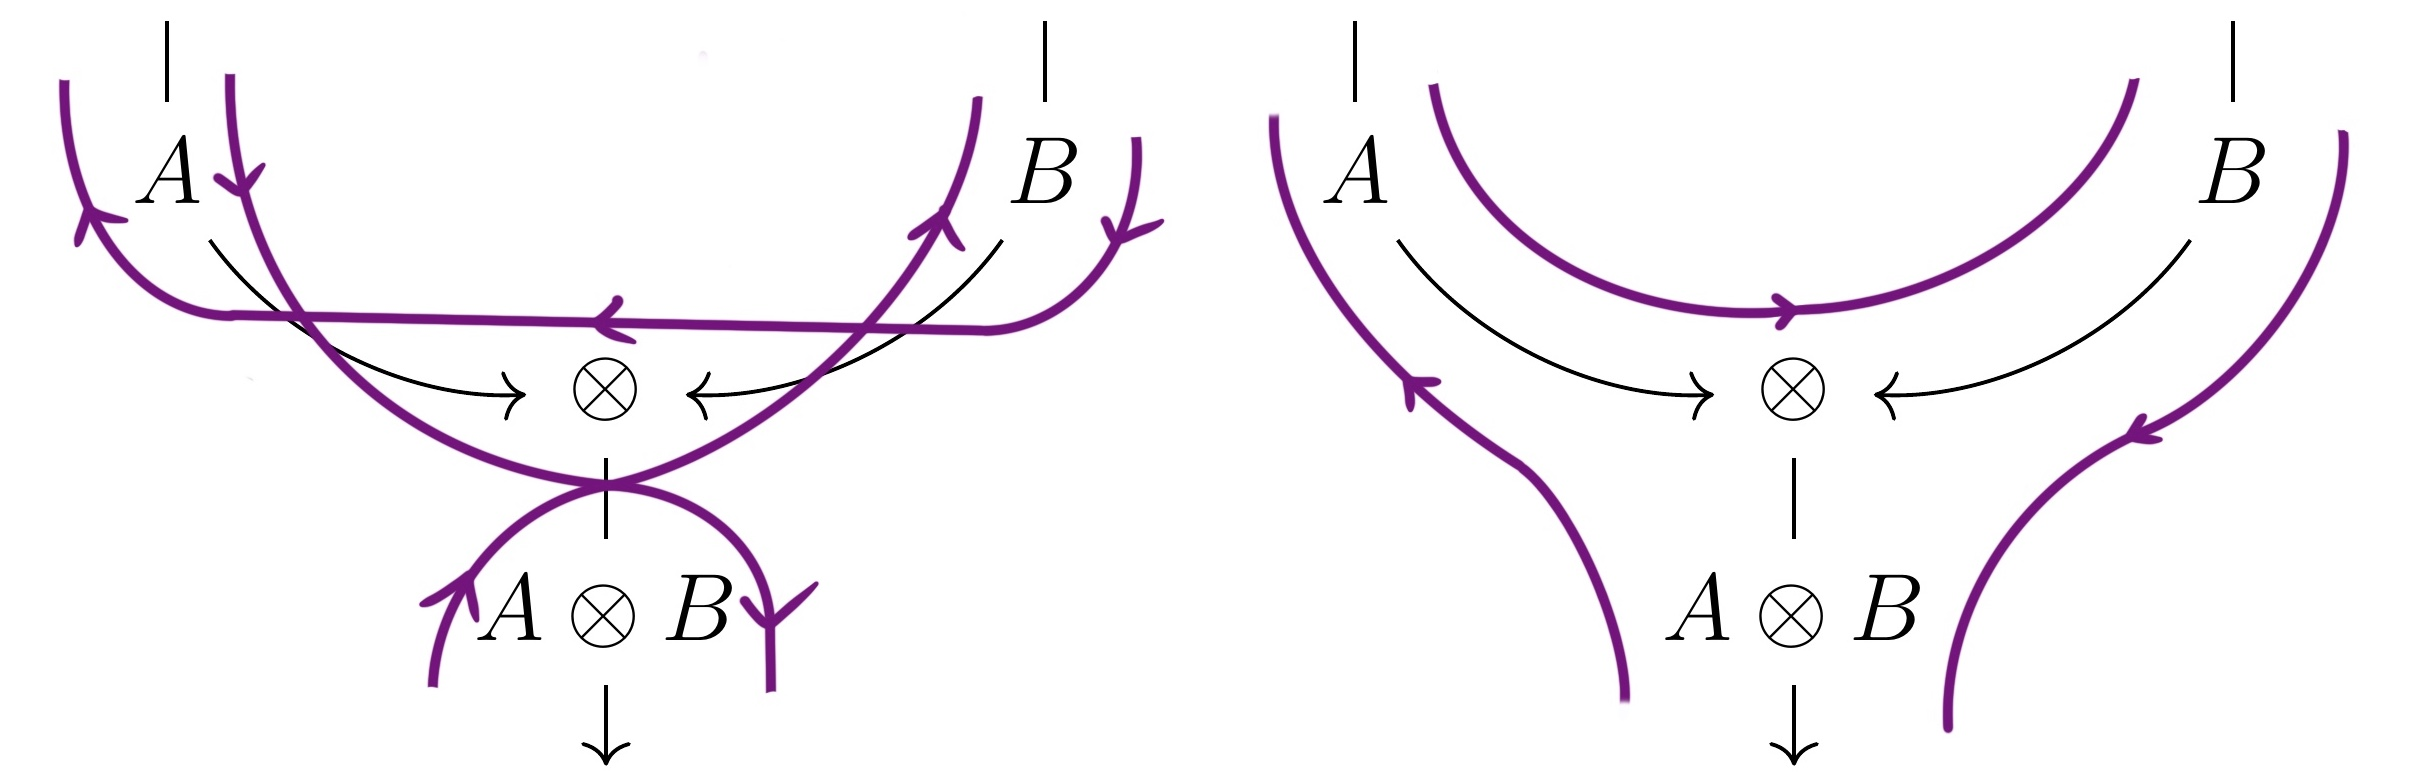
\includegraphics[width = 0.8\textwidth]{TensorSwitch.jpg}
			\caption{Tensor link, $L$ switching, $R$ switching}
			\label{fig:tensorswitching}
		\end{figure}
		\begin{figure}[h]
			\centering
			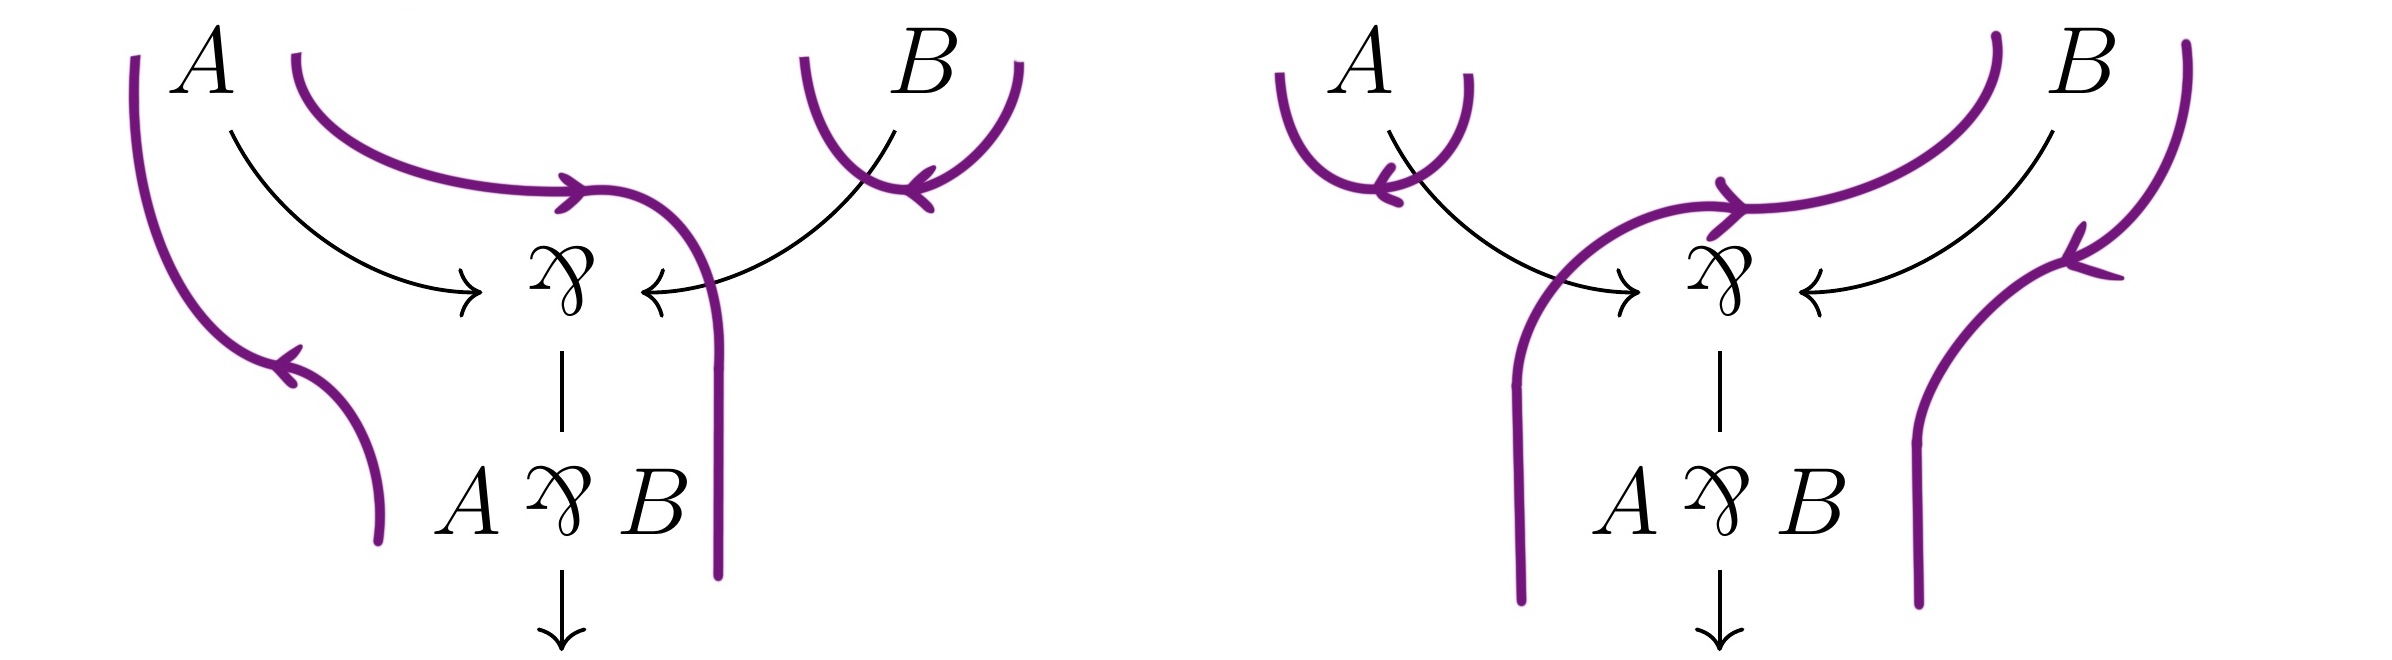
\includegraphics[width = 0.8\textwidth]{ParSwitch.jpg}
			\caption{Par link, $L$ switching, $R$ switching.}
			\label{fig:parrswitching}
		\end{figure}
		\begin{defn}
			Let $\operatorname{Pre}\call{T}(\pi,S)$ denote the set of all pretrips of $\pi$ with respect to $S$. We define an equivalence relation $\sim$ on this set where two pretrips $(x_1,...,x_n)$ and $(y_1,...,y_m)$ are equivalent if $n = m$, and there exists an integer $k$ such that $x_{i + k} = y_i$ (where $i + k$ means $i + k\operatorname{mod} n$) for all $i = 1,...,n$.
			
			A \textbf{trip} of $\pi$ with respect to $S$ is an equivalence class of pretrips. We denote the set of all trips by $\call{T}(\pi,S)$.  If the set $\call{T}(\pi,S)$ admits more than one element, these elements are called \textbf{short trips}, and if it admits only one element, this element is the \textbf{long trip}. We refer to the statement ``for all switchings $S$, the set $\call{T}(\pi,S)$ contains exactly one element" as the \textbf{long trip condition}.
			
			A \textbf{short pretrip} is a choice of representative for a short trip, and a \textbf{long pretrip} is a choice of representatitive of a long trip.
		\end{defn}
		
	\end{defn}
	Given a proof structure $\pi$ satisfying the long trip condition and a tensor link $l$ with premises $A,B$ say, let $S$ be a switching of $\pi$ and $t := (x_1,...,x_n)$ be the long pretrip of $\pi$ satisfying $x_1 =A\downarrow$. Since $\pi$ satisfies the long trip condition, it must be the case that $\uparrow (A \otimes B)$ and $B\downarrow$ occur somewhere in $t$. Can we determine which occurs earlier? Let $m,l > 0$ be such that $x_m = \uparrow (A \otimes B), x_l = B\downarrow$ and assume $l < m$. Say $S(\tau) = L$, then $t$ has the shape
	\begin{equation}\label{eq:sequence_left_switch_tensor}
		(A\downarrow, (A \otimes B)\downarrow, ..., B \downarrow, \uparrow A, ..., \uparrow (A \otimes B), \uparrow B, ..., A\downarrow)
	\end{equation}
	Now consider the switching given by
	\[\hat{S}(\sigma) = \begin{cases}
		S(\sigma),& \sigma \neq \tau\\
		R, & \sigma = \tau
	\end{cases}
	\]
	Then \eqref{eq:sequence_left_switch_tensor} becomes:
	\begin{equation}
		(A\downarrow, \uparrow B, ..., A\downarrow)
	\end{equation}
	which is a short pretrip, contradicting the assumption that $\pi$ satisfies the long trip condition. Thus $m < l$. We have proven (the first half) of the following.
	\begin{lemma}\label{lem:stays_contained_tensor}
		Let $\pi$ be a proof structure satisfying the long trip condition, $l$ be a tensor link with premises $A,B$ say, $S$ be a switching of $\pi$ and $(x_1,...,x_n)$ the long pretrip satisfying $x_1 = A \downarrow$. If $m,l > 0$ are such that $x_m = \uparrow (A \otimes B), x_l = B \downarrow$, then:
		\begin{itemize}
			\item if $S(\tau) = L$ then $m < l$,
			\item if $S(\tau) = R$ then $l < m$.
		\end{itemize}
	\end{lemma}
	The proof of the other half is similar to what has already been written, however since Lemma \ref{lem:stays_contained_tensor} contradicts \cite[Lemma 2.9.1]{linearlogic} we write out the details here:
	\begin{proof}
		Say $m < l$, then $t$ has the shape
		\begin{equation}\label{eq:sequence_right_switch_tensor}
			(A\downarrow, \uparrow B, ..., \uparrow (A \otimes B), \uparrow A, ..., B \downarrow, (A \otimes B)\downarrow, ..., A\downarrow)
		\end{equation}
		Now consider the switching given by
		\[
		S'(\sigma) = 
		\begin{cases}
			S(\sigma),& \sigma \neq \tau\\
			L, & \sigma = \tau
		\end{cases}
		\]
		Then \eqref{eq:sequence_right_switch_tensor} becomes:
		\begin{equation}
			(A\downarrow, (A \otimes B)\downarrow,..., A\downarrow)
		\end{equation}
		which is a short pretrip.
	\end{proof}
	\begin{lemma}\label{lem:stays_contained_par}
		Let $\pi$ be a proof structure satisfying the long trip condition, $l$ be a par link with premises $A,B$ say, $S$ be a switching of $\pi$ and $(x_1,...,x_n)$ be the long pretrip satisfying $x_1 = A\downarrow$. If $m,l > 0$ are such that $x_m = \uparrow (A \parr B), x_l = B\downarrow$, then
		\begin{itemize}
			\item if $S(\tau) = L$ then $m < l$,
			\item if $S(\tau) = R$ then $l < m$
		\end{itemize}
	\end{lemma}
	\begin{remark}
		Lemma \ref{lem:stays_contained_tensor} gives a nice interpretation of Lemma \ref{lem:stays_contained_tensor} that long trips \emph{return to where they left} at each tensor link.
		
		The situation is a bit different for par links; the relevant slogan is long trips \emph{visit the premises before returning to the conclusion}.
	\end{remark}
	Say $\pi$ satisfies the long trip condition and moreover $\pi$ admits a tensor link $l$ (with premises $A,B$ say) such that if $l$ is removed, the resulting proof structure consists of two disjoint proof structures $\pi_1,\pi_2$ each satisfying the long trip condition. It is necessarily the case that any pretrip $\rho$ of $\pi$ starting at $\uparrow A$ visits the entirety of $\call{U}(\pi_1)$ before returning to the tensor link $l$, lest $\pi_1$ admit a short trip. Moreover, it must be the case that $\sigma$ admits no occurrence of formulas in $\pi_2$ lest the result of removing the tensor link $l$ not result in disjoint proof structures. Thus, if such a link $l$ exists, it is \emph{maximal} in the sense that there is no other tensor link $l'$ where a pretrip starting at a premise of $l'$ contains the entirety of any pretrip starting at $A$. Most of the remainder of this Section will amount to proving the converse, that any such maximal tensor link ``splits" $\pi$. This is the \emph{splitting lemma} of \cite{linearlogic}. We then conclude with the Sequentialisation Theorem (Theorem \ref{thm:sequentialisation}).
	\begin{defn}\label{def:pretrip_from_A}
		Let $\pi$ be a proof structure satisfying the long trip condition, $S$ a switching of $\pi$, and $A$ an occurrence of a formula in $\pi$. Consider the long pretrip $(x_1,...,x_n)$ satisfying $x_1 = \uparrow A$. We denote by
		\begin{equation}
			\operatorname{PTrip}(\pi,S,A,\uparrow)
		\end{equation}
		the subsequence $(x_1,...,x_m)$ of $(x_1,...,x_n)$ satisfying $x_m = A\downarrow$. We define
		\begin{equation}
			\operatorname{PTrip}(\pi, S, A, \downarrow)
		\end{equation}
		similarly.
		
		Also, for $a \in \lbrace \uparrow,\downarrow\rbrace $ we define the following set
		\begin{equation}
			\operatorname{Visit}_S(A,a) := \lbrace C \in \call{O}(\pi) \mid \uparrow C, C\downarrow \text{ occur in } \operatorname{PTrip}(\pi,S,A,a)\rbrace
		\end{equation}
		The \textbf{up empire of $A$} is the following set:
		\begin{equation}
			\operatorname{Emp}_{\uparrow}A := \lbrace C \in \call{O}(\pi) \mid \text{For all switchings }S\text{ we have } \uparrow C, C\downarrow \text{ occur in } \operatorname{PTrip}(\pi,S, A,\uparrow)\rbrace
		\end{equation}
		The \textbf{down empire of $A$} is defined symmetrically.
	\end{defn}

One point of difference between the proof presented here and the original proof \cite{linearlogic} is that Girard did \emph{not} consider \emph{down} empires, and instead only considered up empires. At the time of writing, the current author does \emph{not} see how to avoid down empires, and believes the proof in \cite{linearlogic} is too turse to extract a rigorous proof which avoids them.

With the new terminology, we now have some corollaries of Lemmas \ref{lem:stays_contained_tensor} and \ref{lem:stays_contained_par}:
	\begin{cor}\label{cor:pretrip_innards}
		Let $\pi$ be a proof structure satisfying the long trip condition, and let $S$ be a switching of $\pi$, for a formula $A$ and $a \in \lbrace \uparrow, \downarrow\rbrace$, denote $\operatorname{PTrip}(\pi,S, A, a)$ by $\operatorname{PTrip}(A,a)$:
		\begin{enumerate}
			\item if $A$ is part of an axiom link then
			\begin{equation}
				\operatorname{PTrip}(A,\uparrow) = \uparrow A, \operatorname{PTrip}(\neg A, \downarrow), A \downarrow
			\end{equation}
			\item if $l$ is a tensor link with conclusion $A \otimes B$:
			\begin{enumerate}
				\item if $S(l) = L$:
				\begin{equation}
					\operatorname{Ptrip}(A, \downarrow) = A\downarrow, \operatorname{PTrip}(A \otimes B, \downarrow), \operatorname{PTrip}(B, \uparrow), \uparrow A
				\end{equation}
				\begin{equation}
					\operatorname{PTrip}(B, \downarrow) = B\downarrow, \operatorname{PTrip}(A,\uparrow), \operatorname{PTrip}(A \otimes B, \downarrow), \uparrow B
				\end{equation}
				\begin{equation}
					\operatorname{PTrip}(A \otimes B, \uparrow) = \uparrow A \otimes B, \operatorname{PTrip}(B, \uparrow), \operatorname{PTrip}(A,\uparrow), A \otimes B \downarrow
				\end{equation}
				\item if $S(l) = R$:
				\begin{equation}
					\operatorname{PTrip}(A, \downarrow) = A\downarrow, \operatorname{PTrip}(B, \uparrow),\operatorname{PTrip}(A \otimes B, \downarrow), \uparrow A
				\end{equation}
				\begin{equation}
					\operatorname{PTrip}(B, \downarrow) = B\downarrow,  \operatorname{PTrip}(A \otimes B, \downarrow), \operatorname{PTrip}(A,\uparrow),\uparrow B
				\end{equation}
				\begin{equation}
					\operatorname{PTrip}(A \otimes B, \uparrow) = \uparrow A \otimes B,  \operatorname{PTrip}(A,\uparrow), \operatorname{PTrip}(B, \uparrow),A \otimes B \downarrow
				\end{equation}
			\end{enumerate}
			\item if $A$ is a premise of a par link $l$ with conclusion $A \parr B$:
			\begin{enumerate}
				\item if $S(l) = L$:
				\begin{equation}
					\operatorname{PTrip}(A,\downarrow) = A\downarrow, \operatorname{PTrip}(A \parr B, \downarrow), \uparrow A
				\end{equation}
				\begin{equation}
					\operatorname{PTrip}(B, \downarrow) = B\downarrow, \uparrow B
				\end{equation}
				\begin{equation}
					\operatorname{PTrip}(A \parr B, \uparrow) = \uparrow A \parr B, \operatorname{PTrip}(A, \uparrow), A \parr B \downarrow
				\end{equation}
				\item if $S(l) = R$:
				\begin{equation}
					\operatorname{PTrip}(A,\downarrow) = A\downarrow, \uparrow A
				\end{equation}
				\begin{equation}
					\operatorname{PTrip}(B, \downarrow) = B\downarrow, \operatorname{PTrip}(A \parr B, \downarrow), \uparrow B
				\end{equation}
				\begin{equation}
					\operatorname{PTrip}(A \parr B, \uparrow) = \uparrow A \parr B, \operatorname{PTrip}(B, \uparrow), A \parr B \downarrow
				\end{equation}
			\end{enumerate}
		\end{enumerate}
	\end{cor}
	In particular:
	\begin{cor}\label{cor:stays_contained_corollary}
		For any formula $A$ which is a premise to either a tensor or par link, and any $a \in \lbrace \uparrow, \downarrow \rbrace$, we have: $$\uparrow C \text{ occurs in } \operatorname{PTrip}(\pi,S,A,\uparrow)\qquad\text{ if and only if }\qquad C\downarrow \text{ occurs in } \operatorname{PTrip}(\pi,S,A,\downarrow)$$ and similarly for $\operatorname{PTrip}(\pi,S,A,\downarrow)$.
	\end{cor}
	\begin{proof}
		By induction on the length of the sequence $\operatorname{PTrip}(\pi,S,A,a)$ and appealing to Corollary \ref{cor:pretrip_innards}.
	\end{proof}
	\begin{cor}\label{cor:empire_features}
		Let $\pi$ be a proof structure satisfying the long trip condition,
		we have the following.
		\begin{enumerate}
			\item\label{cor:empire_features_up_ax} For any axiom link with conclusions $A, \neg A$:
			\begin{equation}
				\operatorname{Emp}_{\uparrow}A = \operatorname{Emp}_{\downarrow}(\neg A) \cup \lbrace A \rbrace
			\end{equation}
			\item\label{cor:empire_features_down_cut} For any cut link with premises $A, \neg A$:
			\begin{equation}
				\operatorname{Emp}_{\downarrow}A = \operatorname{Emp}_{\uparrow}(\neg A) \cup \lbrace A \rbrace
			\end{equation}
			\item\label{cor:empire_features_empty_int} For any tensor link with premises $A,B$:
			\begin{equation}
				\operatorname{Emp}_{\uparrow}A \cap \operatorname{Emp}_{\uparrow}B = \varnothing
			\end{equation}
			\item\label{cor:empire_features_up_tens_par} For any tensor or par link with premises $A,B$ and conclusion $C$:
			\begin{equation}
				\operatorname{Emp}_{\uparrow}C = \operatorname{Emp}_{\uparrow}A \cup \operatorname{Emp}_{\uparrow}B \cup \lbrace C \rbrace
			\end{equation}
			\item\label{cor:empire_features_down_tens} For any tensor link with premises $A,B$:
			\begin{equation}
				\operatorname{Emp}_{\downarrow}B = \operatorname{Emp}_{\uparrow}A \cup \operatorname{Emp}_{\downarrow}(A \otimes B) \cup \lbrace B \rbrace
			\end{equation}
			and similarly:
			\begin{equation}
				\operatorname{Emp}_{\downarrow}A = \operatorname{Emp}_{\uparrow}B \cup \operatorname{Emp}_{\downarrow}(A \otimes B) \cup \lbrace A\rbrace
			\end{equation}
		\end{enumerate}
	\end{cor}
	\begin{defn}
		Given any link $l$ we write $B \in l$ if $B$ occurs as either a premise or a conclusion of $l$.
		
		Let $\pi$ be a proof structure satisfying the long trip condition, and $a \in \lbrace \uparrow, \downarrow\rbrace$. The set of \textbf{links of $A$ with respect to $S$} is the set
		\begin{equation}
			\operatorname{Link}_aA := \lbrace l \in \operatorname{Link}\pi \mid \forall B \in l, B \in \operatorname{Emp}_aA \rbrace
		\end{equation}
	\end{defn}
	\begin{defn}
		Let $\pi$ be a proof structure satisfying the long trip condition and let $a \in \lbrace \uparrow, \downarrow \rbrace$. Define the set
		\begin{equation}
			\operatorname{Link}^0_{\parr,a}A := \lbrace l \in \operatorname{Link}\pi \mid \text{Exactly one premise of }l\text{ is in }\operatorname{Emp}_{a}A\rbrace
		\end{equation}
	\end{defn}
	\begin{lemma}[Realisation Lemma]\label{lem:realisation_switching}
		Let $\pi$ be a cut-free proof structure satisfying the long trip condition, let $a \in \lbrace \uparrow, \downarrow \rbrace$ and $A$ an occurrence of a formula in $\pi$. Define the following function:
		\begin{align*}
			S: \operatorname{Link}_{\parr,a}^0A &\lto \lbrace L,R\rbrace\\
			l &\longmapsto
			\begin{cases}
				L, & \text{if the right premise of }l\text{ is in }\operatorname{Emp}_{a}A\\
				R, & \text{if the left premise of }l\text{ is in }\operatorname{Emp}_{a}A
			\end{cases}
		\end{align*}
		and extend this to a switching $\hat{S}: \operatorname{Link}\pi \lto \lbrace L,R \rbrace$ arbitrarily. Then
		\begin{equation}
			\operatorname{Emp}_aA = \operatorname{Visit}_{\hat{S}}(A,a)
		\end{equation}
	\end{lemma}
	\begin{proof}
		We proceed by induction on the size $|\operatorname{Link}_a(A)|$ of the set $\operatorname{Link}_a(A)$. For the base case, assume $|\operatorname{Link}_a(A)| = 0$. The formula $A$ is part of an axiom link and so $\operatorname{Emp}_{\uparrow}A = A, \negation A$ and $\operatorname{Emp}_{\downarrow}A = A$, the result follows easily.
		
		Now assume that $|\operatorname{Link}_a A| = n > 0$ and the result holds for any formula $B$ such that $|\operatorname{Link}_aB| < n$. First say $a = \uparrow$, and $A$ is a conclusion of either a tensor or a par link
		% https://q.uiver.app/?q=WzAsNSxbMCwwLCJBXzEiXSxbMiwwLCJBXzIiXSxbMSwxLCJcXGJveHRpbWVzIl0sWzEsMiwiQSJdLFsxLDMsIlxcdmRvdHMiXSxbMyw0XSxbMSwyLCIiLDAseyJjdXJ2ZSI6LTJ9XSxbMCwyLCIiLDIseyJjdXJ2ZSI6Mn1dLFsyLDMsIiIsMCx7InN0eWxlIjp7ImhlYWQiOnsibmFtZSI6Im5vbmUifX19XV0=
		\[\begin{tikzcd}
			{A_1} && {A_2} \\
			& \boxtimes \\
			& A \\
			& \vdots
			\arrow[from=3-2, to=4-2]
			\arrow[curve={height=-12pt}, from=1-3, to=2-2]
			\arrow[curve={height=12pt}, from=1-1, to=2-2]
			\arrow[no head, from=2-2, to=3-2]
		\end{tikzcd}\]
		where $\boxtimes \in \lbrace \otimes, \parr \rbrace$ and $A = A_1 \otimes A_2$ or $A = A_1 \parr A_2$. By \eqref{cor:empire_features_up_tens_par} we have
		\begin{align*}
			\operatorname{Emp}_{\uparrow}A &= \operatorname{Emp}_{\uparrow}A_1 \cup \operatorname{Emp}_{\uparrow}A_2 \cup \lbrace A\rbrace\\
			&= \operatorname{Visit}_{\hat{S}}(A_1,\uparrow) \cup \operatorname{Visit}_S(A_2,\uparrow) \cup \lbrace A \rbrace\\
			&= \operatorname{Visit}_{\hat{S}}(A, \uparrow)
		\end{align*}
		where the second equality follows from the inductive hypothesis.
		
		Assume $A$ is part of an axiom link. By \eqref{cor:empire_features_up_ax}
		\begin{equation}
			\operatorname{Emp}_{\uparrow}A = \operatorname{Emp}_{\downarrow}(\neg A) \cup \lbrace A \rbrace
		\end{equation}
		with
		\begin{equation}
			|\operatorname{Link}_{\uparrow}A| = |\operatorname{Link}_{\downarrow}(\neg A)|
		\end{equation}
		Since $|\operatorname{Link}_{\downarrow}(\negation A)| > 0$ we necessarily have that $\negation A$ is not a conclusion. Thus, since $\pi$ is cut-free, $A$ is connected to an occurrence $\negation A$ which is a premise to either a tensor link or a par link. In the case of the former, we have:
		% https://q.uiver.app/?q=WzAsNSxbMCwwLCJDIl0sWzIsMCwiXFxuZWcgQSJdLFsxLDEsIlxcb3RpbWVzIl0sWzEsMiwiQyBcXG90aW1lcyBcXG5lZyBBIl0sWzEsMywiXFx2ZG90cyJdLFszLDRdLFsxLDIsIiIsMCx7ImN1cnZlIjotMiwic3R5bGUiOnsiaGVhZCI6eyJuYW1lIjoibm9uZSJ9fX1dLFswLDIsIiIsMix7ImN1cnZlIjoyLCJzdHlsZSI6eyJoZWFkIjp7Im5hbWUiOiJub25lIn19fV0sWzIsM11d
		\[\begin{tikzcd}[row sep = small, column sep = small]
			C && {\neg A} \\
			& \otimes \\
			& {C \otimes \neg A} \\
			& \vdots
			\arrow[from=3-2, to=4-2]
			\arrow[curve={height=-12pt}, from=1-3, to=2-2]
			\arrow[curve={height=12pt}, from=1-1, to=2-2]
			\arrow[from=2-2, to=3-2, no head]
		\end{tikzcd}\]
		then by \eqref{cor:empire_features_down_tens}:
		\begin{align*}
			\operatorname{Emp}_{\downarrow}(\neg A) &= \operatorname{Emp}_{\uparrow}C \cup \operatorname{Emp}_{\downarrow}(C \otimes \neg A) \cup \lbrace \neg A\rbrace\\
			&= \operatorname{Visit}_{\hat{S}}(C,\uparrow) \cup \operatorname{Visit}_{\hat{S}}(C \otimes \neg A,\downarrow) \cup \lbrace \neg A\rbrace\\
			&= \operatorname{Visit}_{\hat{S}}(\neg A, \downarrow)
		\end{align*}
		where the second equality follows from the inductive hypothesis.
		
		If $\negation A$ is a premise of a par link
		\[\begin{tikzcd}[column sep = small, row sep = small]
			C && {\neg A} \\
			& \parr \\
			& {C \parr \neg A} \\
			& \vdots
			\arrow[from=3-2, to=4-2]
			\arrow[curve={height=-12pt}, from=1-3, to=2-2]
			\arrow[curve={height=12pt}, from=1-1, to=2-2]
			\arrow[from=2-2, to=3-2, no head]
		\end{tikzcd}\]
		then by construction of $\hat{S}$, where we use the specific definition of $S$ for the first time,
		\begin{align*}
			\operatorname{Emp}_{\downarrow}(\neg A) &= \lbrace \neg A\rbrace\\
			&= \operatorname{Visit}_{\hat{S}}(\neg A,\downarrow)
		\end{align*}
		The case when $a = \downarrow$ is exactly similar and so we omit the proof.
	\end{proof}
	\begin{defn}
		A tensor or par link is \textbf{terminal} if it is a conclusion.
	\end{defn}
	\begin{cor}\label{lem:par_link_existence}
		Let $\pi$ be a cut-free proof structure satisfying the long trip condition. Let
		\[l = \begin{tikzcd}[column sep = small, row sep = small]
			A && {B} \\
			& \otimes \\
			& {A \otimes B} \\
			& \operatorname{c}
			\arrow[from=3-2, to=4-2]
			\arrow[curve={height=-12pt}, from=1-3, to=2-2]
			\arrow[curve={height=12pt}, from=1-1, to=2-2]
			\arrow[from=2-2, to=3-2, no head]
		\end{tikzcd}\]
		be a terminal tensor link of $\pi$. Then $\pi$ admits a par link
		\[l' := \begin{tikzcd}[column sep = small, row sep = small]
			C && {D} \\
			& \otimes \\
			& {C \parr D} \\
			& \vdots
			\arrow[from=3-2, to=4-2]
			\arrow[curve={height=-12pt}, from=1-3, to=2-2]
			\arrow[curve={height=12pt}, from=1-1, to=2-2]
			\arrow[from=2-2, to=3-2, no head]
		\end{tikzcd}\]
		such that either $C \in \operatorname{Emp}_{\uparrow}A$ and $D \in \operatorname{Emp}_{\uparrow}B$ or $C \in \operatorname{Emp}_{\uparrow}B$ and $D \in \operatorname{Emp}_{\uparrow}A$ if and only if for any switching $S$ of $\pi$ we have that either
		\[\operatorname{Emp}_{\uparrow}A \subsetneq \operatorname{Visit}_S(A,\uparrow)\qquad\text{or}\qquad \operatorname{Emp}_{\uparrow}B \subsetneq \operatorname{Visit}_S(B,\uparrow)\]
	\end{cor}
	\begin{proof}
		Say $\pi$ admitted $l'$ and $C \in \operatorname{Emp}_{\uparrow}A$ and $D \in \operatorname{Emp}_{\uparrow}B$. If the switching $S$ is such that $S(l) = L$ then $C \parr D \in \operatorname{Visit}_S(B)\setminus \operatorname{Emp}_{\uparrow}B$ and if $S(\tau) = R$ then $C \parr D \in \operatorname{Visit}_S(A) \setminus \operatorname{Emp}_{\uparrow}A$. The other case is similar.
		
		Conversely, say $\pi$ admits no such par link $l'$, that is, assume
		\begin{equation}
			\operatorname{Link}^0_{\parr,\uparrow}(A) \cap \operatorname{Link}^0_{\parr,\uparrow}(B) = \varnothing
		\end{equation}
		Then there is by Lemma \ref{lem:realisation_switching} a well defined function $$S: \operatorname{Link}_{\parr,\uparrow}^0(A) \cup \operatorname{Link}^0_{\parr,\uparrow}(B) \lto \lbrace L, R \rbrace$$ which extends to a switching $\hat{S}$ such that
		\begin{equation}
			\operatorname{Emp}_{\uparrow}A = \operatorname{Visit}_{\hat{S}}(A,\uparrow)\qquad\text{and}\qquad \operatorname{Emp}_{\uparrow}B = \operatorname{Visit}_{\hat{S}}(B,\uparrow)
		\end{equation}
	\end{proof}
	
	\begin{lemma}[Separation Lemma]
		A cut-free proof structure $\pi$ satisfying the long trip condition, with only tensor links amongst its conclusions admits a tensor link
		\[l := \begin{tikzcd}[column sep = small, row sep = small]
			A && {B} \\
			& \otimes \\
			& {A \otimes B} \\
			& \operatorname{c}
			\arrow[from=3-2, to=4-2]
			\arrow[curve={height=-12pt}, from=1-3, to=2-2]
			\arrow[curve={height=12pt}, from=1-1, to=2-2]
			\arrow[from=2-2, to=3-2, no head]
		\end{tikzcd}\]
		satisfying
		\begin{equation}
			\call{O}(\pi) = \operatorname{Emp}_{\uparrow}A \cup \operatorname{Emp}_{\uparrow}B \cup \lbrace A \otimes B\rbrace
		\end{equation}
		Moreover, removing $A \otimes B$ results in a disconnected graph with each component a proof structure satisfying the long trip condition.
	\end{lemma}
	\begin{proof}
		Consider the set of tensor links $\operatorname{Link}_{\otimes}(\pi)$ of $\pi$. We endow this with the following partial order $\leq$: a pair of links:
		\[
		l' := \begin{tikzcd}[column sep = small, row sep = small]
			A && {B} \\
			& \otimes \\
			& {A \otimes B} \\
			& \vdots
			\arrow[from=3-2, to=4-2]
			\arrow[curve={height=-12pt}, from=1-3, to=2-2]
			\arrow[curve={height=12pt}, from=1-1, to=2-2]
			\arrow[from=2-2, to=3-2, no head]
		\end{tikzcd}
		%
		\qquad
		%
		l'' :=
		\begin{tikzcd}[column sep = small, row sep = small]
			C && {D} \\
			& \otimes \\
			& {C \otimes D} \\
			& \vdots
			\arrow[from=3-2, to=4-2]
			\arrow[curve={height=-12pt}, from=1-3, to=2-2]
			\arrow[curve={height=12pt}, from=1-1, to=2-2]
			\arrow[from=2-2, to=3-2, no head]
		\end{tikzcd}
		\]
		are such that $l' \leq l''$ if $\operatorname{Emp}_{\uparrow}A \cup \operatorname{Emp}_{\uparrow}B \subseteq \operatorname{Emp}_{\uparrow}C \cup \operatorname{Emp}_{\uparrow}D$. Let $l$ (with conclusion $A \otimes B$ say) be a tensor link maximal with respect to $\leq$. We show that $l$ satisfies the required property.
		
		Say $\call{O}(\pi) \neq \operatorname{Emp}_{\uparrow}A \cup \operatorname{Emp}_{\uparrow}B \cup \lbrace A \otimes B\rbrace$. Then by Lemma \ref{lem:par_link_existence} there exists a par link
		\[
		l' = \begin{tikzcd}[column sep = small, row sep = small]
			C && {D} \\
			& \parr \\
			& {C \parr D} \\
			& \vdots
			\arrow[from=3-2, to=4-2]
			\arrow[curve={height=-12pt}, from=1-3, to=2-2]
			\arrow[curve={height=12pt}, from=1-1, to=2-2]
			\arrow[from=2-2, to=3-2, no head]
		\end{tikzcd}
		\]
		such that either $C \in \operatorname{Emp}_{\uparrow}A$ and $D \in \operatorname{Emp}_{\uparrow}B$ or $C \in \operatorname{Emp}_{\uparrow}B$ and $D \in \operatorname{Emp}_{\uparrow}A$. We show the proof in the case of the former. Since $\pi$ admits no terminal par links, the unique maximal length directed path of $\pi$ beginning at the node $\parr$ of $l'$ terminates at an edge labelled $E \otimes F$, for some $E,F$.
		\[l'':= \begin{tikzcd}[column sep = small, row sep = small]
			E && {F} \\
			& \otimes \\
			& {E \otimes F} \\
			& \vdots
			\arrow[from=3-2, to=4-2]
			\arrow[curve={height=-12pt}, from=1-3, to=2-2]
			\arrow[curve={height=12pt}, from=1-1, to=2-2]
			\arrow[from=2-2, to=3-2, no head]
		\end{tikzcd}\]
		Notice that if $l'' = l$, then either $C \parr D \in \operatorname{Emp}_{\uparrow}A$ or $C \parr D \in \operatorname{Emp}_{\uparrow}B$ which in either case implies $\operatorname{Emp}_{\uparrow}A \cap \operatorname{Emp}_{\uparrow}B \neq \varnothing$, contradicting Corollary \ref{cor:empire_features}, \ref{cor:empire_features_empty_int}, and so $l'' \neq l$. Without any loss of generality, assume that $l'$ sits above $F$. The situation looks as follows.
		% https://q.uiver.app/?q=WzAsMjEsWzMsMywiQSBcXG90aW1lcyBCIl0sWzMsNSwiXFxvcGVyYXRvcm5hbWV7Y30iXSxbMiwyLCJBIl0sWzIsMSwiXFx2ZG90cyJdLFsxLDAsIlxcYXgiXSxbMCw1LCJDIl0sWzMsNiwiXFxwYXJyIl0sWzYsNSwiRCJdLFszLDcsIkMgXFxwYXJyIEQiXSxbMCwxLCJcXHZkb3RzIl0sWzQsMiwiQiJdLFs0LDEsIlxcdmRvdHMiXSxbNSwwLCJcXGF4Il0sWzYsMSwiXFx2ZG90cyJdLFszLDgsIlxcdmRvdHMiXSxbMyw5LCJGIl0sWzIsMTAsIlxcb3RpbWVzIl0sWzIsMTIsIlxcb3BlcmF0b3JuYW1le2N9Il0sWzIsMTEsIkUgXFxvdGltZXMgRiJdLFsxLDksIkUiXSxbMSw4LCJcXHZkb3RzIl0sWzAsMV0sWzIsMCwiIiwwLHsiY3VydmUiOjJ9XSxbMywyLCIiLDAseyJzdHlsZSI6eyJoZWFkIjp7Im5hbWUiOiJub25lIn19fV0sWzQsMywiIiwwLHsiY3VydmUiOi0yfV0sWzUsNiwiIiwwLHsiY3VydmUiOjJ9XSxbNyw2LCIiLDIseyJjdXJ2ZSI6LTJ9XSxbNiw4LCIiLDIseyJzdHlsZSI6eyJoZWFkIjp7Im5hbWUiOiJub25lIn19fV0sWzQsOSwiIiwyLHsiY3VydmUiOjJ9XSxbOSw1LCIiLDEseyJzdHlsZSI6eyJoZWFkIjp7Im5hbWUiOiJub25lIn19fV0sWzEyLDExLCIiLDEseyJjdXJ2ZSI6Mn1dLFsxMiwxMywiIiwxLHsiY3VydmUiOi0yfV0sWzEzLDcsIiIsMSx7InN0eWxlIjp7ImhlYWQiOnsibmFtZSI6Im5vbmUifX19XSxbOCwxNF0sWzIwLDE5LCIiLDIseyJzdHlsZSI6eyJoZWFkIjp7Im5hbWUiOiJub25lIn19fV0sWzE5LDE2LCIiLDIseyJjdXJ2ZSI6Mn1dLFsxNSwxNiwiIiwwLHsiY3VydmUiOi0yfV0sWzE2LDE4LCIiLDAseyJzdHlsZSI6eyJoZWFkIjp7Im5hbWUiOiJub25lIn19fV0sWzE4LDE3XSxbMTQsMTUsIiIsMSx7InN0eWxlIjp7ImhlYWQiOnsibmFtZSI6Im5vbmUifX19XSxbMTEsMTAsIiIsMSx7InN0eWxlIjp7ImhlYWQiOnsibmFtZSI6Im5vbmUifX19XSxbMTAsMCwiIiwxLHsiY3VydmUiOi0yfV1d
		\[\begin{tikzcd}[column sep = small, row sep = small]
			& \ax &&&& \ax \\
			\vdots && \vdots && \vdots && \vdots \\
			&& A && B \\
			&&& {A \otimes B} \\
			\\
			C &&& {\operatorname{c}} &&& D \\
			&&& \parr \\
			&&& {C \parr D} \\
			& \vdots && \vdots \\
			& E && F \\
			&& \otimes \\
			&& {E \otimes F} \\
			&& {\operatorname{c}}
			\arrow[from=4-4, to=6-4]
			\arrow[curve={height=12pt}, from=3-3, to=4-4]
			\arrow[no head, from=2-3, to=3-3]
			\arrow[curve={height=-12pt}, from=1-2, to=2-3]
			\arrow[curve={height=12pt}, from=6-1, to=7-4]
			\arrow[curve={height=-12pt}, from=6-7, to=7-4]
			\arrow[no head, from=7-4, to=8-4]
			\arrow[curve={height=12pt}, from=1-2, to=2-1]
			\arrow[no head, from=2-1, to=6-1]
			\arrow[curve={height=12pt}, from=1-6, to=2-5]
			\arrow[curve={height=-12pt}, from=1-6, to=2-7]
			\arrow[no head, from=2-7, to=6-7]
			\arrow[from=8-4, to=9-4]
			\arrow[no head, from=9-2, to=10-2]
			\arrow[curve={height=12pt}, from=10-2, to=11-3]
			\arrow[curve={height=-12pt}, from=10-4, to=11-3]
			\arrow[no head, from=11-3, to=12-3]
			\arrow[from=12-3, to=13-3]
			\arrow[no head, from=9-4, to=10-4]
			\arrow[no head, from=2-5, to=3-5]
			\arrow[curve={height=-12pt}, from=3-5, to=4-4]
		\end{tikzcd}\]
		
		
		
		Let $S$ be a switching of $\pi$ so that $\operatorname{Emp}_{\uparrow}F = \operatorname{Visit}_S(F,\uparrow)$ and so that $S(l') = L$, which exists by Lemma \ref{lem:par_link_existence}. Let $t = (x_1,...,x_n)$ be the long pretrip of $\pi$ with respect to $S$ satisfying $x_1 = F\uparrow$. We have by Lemma \ref{lem:stays_contained_par} that $t$ takes the following shape:
		\begin{equation}\label{eq:condemning_shape}
			\uparrow F, ..., \uparrow(C \parr D), \uparrow C, ..., D\downarrow, \uparrow D, ..., C\downarrow, (C \parr D)\downarrow, ..., F\downarrow,...
		\end{equation}
		We have that $D \in \operatorname{Emp}_{\uparrow}B$ so for simplicity, rewrite \eqref{eq:condemning_shape} as $t' = (x_{1 + k},...,x_{n+k})$ for some $k > 0$ (where $i + k$ means $i + k\operatorname{mod} n$) so that $\uparrow B$ occurs to the left of $D \downarrow$ and $B \downarrow$ occurring to the right of $\uparrow D$.
		We have that $C \not\in \operatorname{Emp}_{\uparrow}B$ and so by Corollary \ref{cor:stays_contained_corollary}:
		\begin{equation}
			\uparrow B \text{ occurrs in }\uparrow C,..., D\downarrow\text{ and } B\downarrow\text{ occurrs in }\uparrow D, ..., C\downarrow
		\end{equation}
		However, this implies that $B \in \operatorname{Visit}_S(F,\uparrow)$ which by Lemma \ref{lem:realisation_switching} implies $B \in \operatorname{Emp}_{\uparrow}F$.
		
		By reversing the switching of $l'$ we can similarly show that $A \in \operatorname{Emp}_{\uparrow}F$, contradicting the maximality of $l$. This proves the first claim.
		
		For the second claim, since $\call{O}(\pi) = \operatorname{Emp}_{\uparrow}A \cup \operatorname{Emp}_{\uparrow}B \cup \lbrace A \otimes B\rbrace$ we have by Lemma \ref{lem:par_link_existence} that
		\begin{equation}
			\operatorname{Link}_{\parr,\uparrow}^0(A\otimes B) = \varnothing
		\end{equation}
		and we saw in the proof of Lemma \ref{lem:realisation_switching} that a switching $S$ which realises $\operatorname{Emp}_{\uparrow}A$ is given by setting all switchings arbitrarily except for those in $\operatorname{Link}_{\parr,\uparrow}^0(A\otimes B)$. This means that for any switching $S$ of $\pi$:
		\begin{equation}
			\operatorname{Visit}_{S}(A,\uparrow) = \operatorname{Emp}_{\uparrow}A \qquad\text{and}\qquad \operatorname{Visit}_{S}(B,\uparrow) = \operatorname{Emp}_{\uparrow}B
		\end{equation}
		which is to say the two subproof structures given by removing $A \otimes B$ never admit a short trip, that is, they each satisfy the long trip condition.
	\end{proof}
	\begin{thm}[The Sequentialisation Theorem]\label{thm:sequentialisation}
		A proof structure $\pi$ (possibly with cuts) satisfies the long trip condition if and only $\pi$ is a proof net.
	\end{thm}
	\begin{proof}
		First assume that $\pi$ is cut-free.
		
		We proceed by induction on the size $|\operatorname{Link}\pi|$ of the set $\operatorname{Link}\pi$. If there this is zero then $\pi$ consists of a single axiom link and so the result is clear.
		
		For the inductive step, we consider two cases, first say $\pi$ admits a par link for a conclusion. Then removing this par link clearly results in two cut-free subproof structures satsifying the long trip condition and so the result follows from the inductive hypothesis. If no such terminal par link exists, then by the Separation Lemma there exists some tensor link in the conclusion for which we can remove and apply the inductive hypothesis.
		
		Now say that $\pi$ contained cuts. We replace each cut with a tensor link to create a new proof $\zeta$. That there exists a proof $\Xi$ which maps to $\zeta$ follows from the part of the result proved already as $\zeta$ is cut-free. We adapt $\Xi$ appropriately by replacing $\otimes$-rules by $\operatorname{cut}$-rules and we are done.
	\end{proof}

\section{The dynamics of MLL}\label{sec:dynamics}

Linear logic is a \emph{dynamic} system, in that it involves a proof \emph{re-write} procedure. This procedure is the \emph{cut-elimination} process and constitutes the content of this section.

\begin{defn}
	A subgraph of a proof structure $\pi$ of one of the following forms is an \emph{$a$-redex}.
	\begin{center}
		\begin{tabular}{ c c c }
			$
			\begin{tikzcd}[column sep = small, row sep = small]
				& \ax\arrow[dr,bend left, dash]\arrow[dl,bend right, dash] &&& \vdots\arrow[d,dash]\\
				\neg A\arrow[d] && A\arrow[dr,bend right] && \neg A\arrow[dl,bend left]\\
				\vdots&&&\cut
			\end{tikzcd}
			$
			&
			$
			\begin{tikzcd}[column sep = small, row sep = small]
				\vdots\arrow[d,dash] &&& \ax\arrow[dl, bend right, dash]\arrow[dr,dash, bend left]\\
				A\arrow[dr, bend right] && \neg A\arrow[dl,bend left] && A\arrow[d]\\
				& \cut &&& \vdots
			\end{tikzcd}
			$
			&
			\tagarray{\label{eq:a_redex}}
		\end{tabular}
	\end{center}
	A subgraph of a proof structure of the following form is an \emph{$m$-redex}.
	\begin{center}
		\begin{tabular}{ c c }
			$
			% https://q.uiver.app/?q=WzAsMTQsWzAsMF0sWzIsMSwiQSJdLFszLDIsIlxcb3RpbWVzIl0sWzQsMSwiQiJdLFs2LDAsInZfMyJdLFs2LDEsIlxcbmVnIEEiXSxbNywyLCJcXHBhcnIiXSxbOCwxLCJcXG5lZyBCIl0sWzgsMCwidl80Il0sWzMsMywiQSBcXG90aW1lcyBCIl0sWzcsMywiXFxuZWcgQSBcXHBhcnIgXFxuZWcgQiJdLFs1LDQsIlxcY3V0Il0sWzIsMCwidl8xIl0sWzQsMCwidl8yIl0sWzEsMiwiIiwwLHsiY3VydmUiOjJ9XSxbMywyLCIiLDAseyJjdXJ2ZSI6LTJ9XSxbNSw2LCIiLDAseyJjdXJ2ZSI6Mn1dLFs3LDYsIiIsMCx7ImN1cnZlIjotMn1dLFs0LDUsIiIsMix7InN0eWxlIjp7ImhlYWQiOnsibmFtZSI6Im5vbmUifX19XSxbOCw3LCIiLDAseyJzdHlsZSI6eyJoZWFkIjp7Im5hbWUiOiJub25lIn19fV0sWzYsMTAsIiIsMCx7InN0eWxlIjp7ImhlYWQiOnsibmFtZSI6Im5vbmUifX19XSxbOSwxMSwiIiwwLHsiY3VydmUiOjJ9XSxbMTAsMTEsIiIsMSx7ImN1cnZlIjotMn1dLFsyLDksIiIsMSx7InN0eWxlIjp7ImhlYWQiOnsibmFtZSI6Im5vbmUifX19XSxbMTIsMSwiIiwwLHsic3R5bGUiOnsiaGVhZCI6eyJuYW1lIjoibm9uZSJ9fX1dLFsxMywzLCIiLDAseyJzdHlsZSI6eyJoZWFkIjp7Im5hbWUiOiJub25lIn19fV1d
			\begin{tikzcd}[column sep = small, row sep = small]
				{} && {\vdots} && {\vdots} && {\vdots} && {\vdots} \\
				&& A && B && {\neg A} && {\neg B} \\
				&&& \otimes &&&& \parr \\
				&&& {A \otimes B} &&&& {\neg A \parr \neg B} \\
				&&&&& \cut
				\arrow[curve={height=12pt}, from=2-3, to=3-4]
				\arrow[curve={height=-12pt}, from=2-5, to=3-4]
				\arrow[curve={height=12pt}, from=2-7, to=3-8]
				\arrow[curve={height=-12pt}, from=2-9, to=3-8]
				\arrow[no head, from=1-7, to=2-7]
				\arrow[no head, from=1-9, to=2-9]
				\arrow[no head, from=3-8, to=4-8]
				\arrow[curve={height=12pt}, from=4-4, to=5-6]
				\arrow[curve={height=-12pt}, from=4-8, to=5-6]
				\arrow[no head, from=3-4, to=4-4]
				\arrow[no head, from=1-3, to=2-3]
				\arrow[no head, from=1-5, to=2-5]
			\end{tikzcd}
			$
			&
			\tagarray{\label{eq:m_redex}}
		\end{tabular}
	\end{center}
\end{defn}


\begin{defn}\label{def:reduction}
	Multiplicative linear logic proof structures come equipped with three reduction rules, these reduction rules apply to proofs which admit either an $a$-redex or an $m$-redex. More precisely, given a multiplicative linear logic proof structure $\pi$ admitting an $a$-redex $\zeta$ of the form given on the left in \eqref{rule:ax_reduct_negation}, the reduction of $\pi$ is the proof $\pi'$ given by replacing the subgraph $\zeta$ in $\pi$ by what is displayed on the right in \eqref{rule:ax_reduct_negation}. Similarly for if $\pi$ admits an $a$-redex of the form given on the left of \eqref{rule:ax_reduct} or if $\pi$ admits an $m$-redex.
	\begin{center}
		\begin{tabular}{ c c c }
			$
			\begin{tikzcd}[column sep = small, row sep = small]
				& \ax\arrow[dr,bend left, dash]\arrow[dl,bend right, dash] &&& \vdots\arrow[d,dash]\\
				\neg A\arrow[d] && A\arrow[dr,bend right] && \neg A\arrow[dl,bend left]\\
				\vdots&&&\cut
			\end{tikzcd}
			$
			&
			$
			\begin{tikzcd}[column sep = small, row sep = small]
				\vdots\arrow[d,dash]\\
				\neg A\arrow[d]\\
				\vdots
			\end{tikzcd}
			$
			&
			\tagarray{\label{rule:ax_reduct_negation}}\\
			$
			\begin{tikzcd}[column sep = small, row sep = small]
				\vdots\arrow[d,dash] &&& \ax\arrow[dl, bend right, dash]\arrow[dr,dash, bend left]\\
				A\arrow[dr, bend right] && \neg A\arrow[dl,bend left] && A\arrow[d]\\
				& \cut &&& \vdots
			\end{tikzcd}
			$
			&
			$
			\begin{tikzcd}[column sep = small, row sep = small]
				\vdots\arrow[d,dash]\\
				A\arrow[d]\\
				\vdots
			\end{tikzcd}
			$
			&
			\tagarray{\label{rule:ax_reduct}}
		\end{tabular}
	\end{center}
	
	\begin{center}
		\begin{tabular}{ c c }
			$\begin{tikzcd}[column sep = small, row sep = small]
				\vdots && \vdots && \vdots && \vdots \\
				A && B && {\neg A} && {\neg B} \\
				& \otimes &&&& \parr \\
				& {A \otimes B} &&&& {\neg A \parr \neg B} \\
				&&& \cut
				%			\arrow[curve={height=12pt}, from=4-2, to=5-4]
				%			\arrow[curve={height=-12pt}, from=4-6, to=5-4]
				\arrow[from=2-5, to=3-6]
				\arrow[from=2-7, to=3-6]
				\arrow[from=3-6, to=4-6, dash]
				\arrow[from=3-2, to=4-2, dash]
				\arrow[from=2-1, to=3-2]
				\arrow[from=2-3, to=3-2]
				\arrow[from=1-1, to=2-1, dash]
				\arrow[from=1-3, to=2-3, dash]
				\arrow[from=1-5, to=2-5, dash]
				\arrow[from=1-7, to=2-7, dash]
				\arrow[from=4-2, to=5-4, bend right]
				\arrow[from=4-6, to=5-4, bend left]
			\end{tikzcd}$\\
			& \tagarray{\label{rule:tensor_reduct}}\\
			$\begin{tikzcd}[column sep = small, row sep = small]
				\vdots && \vdots && \vdots && \vdots \\
				A && B && {\neg A} && {\neg B} \\
				& \cut &&&& \cut
				\arrow[from=1-1, to=2-1, dash]
				\arrow[from=1-3, to=2-3, dash]
				\arrow[from=1-5, to=2-5, dash]
				\arrow[from=1-7, to=2-7, dash]
				\arrow[from=2-1, to=3-2, bend right]
				\arrow[from=2-5, to=3-2, bend left]
				\arrow[from=2-3, to=3-6, bend right]
				\arrow[from=2-7, to=3-6, bend left]
			\end{tikzcd}$
		\end{tabular}
	\end{center}
	A \textbf{reduction} is a pair of proof structures $(\pi,\pi')$ where $\pi'$ is the result of applying one of the reduction rules just described to $\pi$. We write $\pi \lto_{\cut} \pi'$ when $(\pi,\pi')$ is a reduction.
\end{defn}
\begin{proposition}[Church-Rosser/confluence]\label{prop:church_rosser}
	If $\pi_1$ is a proof structure and $\pi_1 \lto_{\operatorname{cut}} \pi_2, \pi_1 \lto_{\operatorname{cut}} \pi_3$ then there exists a proof structure $\pi_4$ such that $\pi_2 \lto_{\operatorname{cut}} \pi_4, \pi_3 \lto_{\operatorname{cut}} \pi_4$.
\end{proposition}
\begin{proof}[Proof sketch]
	The key observation is that reducing any redex in a proof does not eliminate any other redex.
\end{proof}
\begin{defn}
	Let $\pi$ be a proof net possibly containing cut links. A \textbf{reduction sequence} is a sequence
	\begin{equation}
		\pi = \pi_0 \lto_{\operatorname{cut}} \pi_1 \lto_{\operatorname{cut}} \hdots \lto_{\operatorname{cut}} \pi_n
	\end{equation}
	with $\pi_n$ cut-free.
\end{defn}
\begin{lemma}\label{lem:red_sequence_existence}
	Every proof net $\pi$ admits a reduction sequence.
\end{lemma}
\begin{proof}
	Given a cut link $l$ with premises $\neg A, A$ say, the \textbf{complexity of $l$}, $c(l)$ is the sum of the number of occurrences of $\otimes$ and the number of occurrences of $\parr$ in $A$. We proceed by induction on the maximum of the complexities of all cut links in $\pi$.
	
	Say this maximum is $0$. Then all cut-links have the shape of either \eqref{rule:ax_reduct_negation} or \eqref{rule:ax_reduct}. We can reduce these redexes (in any order) to deduce the result.
	
	Now say the maximum is $n > 0$. We then apply \eqref{rule:tensor_reduct} to all cut links of complexity $n$ (in any order) to obtain a new proof structure $\zeta$. We wish to use the inductive hypothesis on $\zeta$ but we must make sure that $\zeta$ satisfies the longtrip condition. This follows easily by considering the contrapositive: any pretrip (long or short) of $\zeta$ appears as a subsequent of some pretrip of $\pi$, so if $\zeta$ admits a short trip so does $\pi$. We can now apply the inductive hypothesis and we are done.
\end{proof}
\begin{defn}
	Let $\operatorname{Red}\pi$ denote the set of all reduction sequences of $\pi$. The \textbf{length} $l(\underline{x})$ of a reduction sequence $\underline{x} \in \operatorname{Red}\pi$ is the length of the sequence $\underline{x}$.
\end{defn}
\begin{cor}\label{cor:stable_length}
	The length of a reduction path is independent of the choice of reduction path.
\end{cor}
\begin{proof}
	The proof is purely geometric. Let
	\begin{equation}
		\underline{x} := ( \pi = \pi_1 \lto_{\operatorname{cut}} \hdots \lto_{\operatorname{cut}} \pi_n)
	\end{equation}
	be the reduction path described by Lemma \ref{lem:red_sequence_existence} and let
	\begin{equation}
		\underline{y} := (\pi = \zeta_0 \lto_{\operatorname{cut}} \hdots \lto_{\operatorname{cut}} \zeta_n)
	\end{equation}
	be any other reduction sequence. By Lemma \ref{prop:church_rosser} we have $\pi_n = \zeta_n$. Also using \ref{prop:church_rosser}, the pair of reduction paths can be completed to some grid defined by a subset of $\bb{N} \times \bb{N}$. All paths $p$ consisting of only upwards steps or right steps such that $p$ is bound to this grid have the same length and so $l(\underline{x}) = l(\underline{y})$.
\end{proof}
\begin{defn}\label{def:normal_form}
	The proof of Corollary \ref{cor:stable_length} shows that every reduction path of a proof net $\pi$ leads to the same cut-free proof $\zeta$. We call $\zeta$ the \textbf{normal form} of $\pi$.
\end{defn}
\begin{defn}\label{def:eta_expansion}
	A pair of proof nets $(\pi,\pi')$ where $\pi'$ is obtained from $\pi$ via replacing some subgraph of $\pi$ of the form on the left of \eqref{eq:eta_expansion} is an \textbf{$\eta$-expansion}. We write $\pi \lto_{\eta} \pi'$. An \textbf{$\eta$-increx} is a subgraph of a proof structure of the form given on the left of \eqref{eq:eta_expansion}.
\end{defn}
% https://q.uiver.app/?q=WzAsNSxbMSwwLCJcXGF4Il0sWzIsMSwiXFxuZWcgQSBcXHBhcnIgXFxuZWcgQiJdLFswLDEsIkEgXFxvdGltZXMgQiJdLFswLDIsIlxcdmRvdHMiXSxbMiwyLCJcXHZkb3RzIl0sWzAsMSwiIiwyLHsiY3VydmUiOi0yLCJzdHlsZSI6eyJoZWFkIjp7Im5hbWUiOiJub25lIn19fV0sWzAsMiwiIiwwLHsiY3VydmUiOjIsInN0eWxlIjp7ImhlYWQiOnsibmFtZSI6Im5vbmUifX19XSxbMiwzXSxbMSw0XV0=
\begin{equation}\label{eq:eta_expansion}
	\begin{tikzcd}[column sep = small, row sep = small]
		& \ax \\
		{A \otimes B} && {\neg A \parr \neg B} \\
		\vdots && \vdots
		\arrow[curve={height=-12pt}, no head, from=1-2, to=2-3]
		\arrow[curve={height=12pt}, no head, from=1-2, to=2-1]
		\arrow[from=2-1, to=3-1]
		\arrow[from=2-3, to=3-3]
	\end{tikzcd}
	% https://q.uiver.app/?q=WzAsMTIsWzEsMCwiXFxheCJdLFswLDEsIkEiXSxbMiwxLCJcXG5lZyBBIl0sWzQsMCwiXFxheCJdLFszLDEsIkIiXSxbNSwxLCJcXG5lZyBCICJdLFsxLDIsIlxcb3RpbWVzIl0sWzMsMiwiXFxwYXJyIl0sWzMsMywiXFxuZWcgQSBcXHBhcnIgXFxuZWcgQiJdLFszLDQsIlxcdmRvdHMiXSxbMSwzLCJBIFxcb3RpbWVzIEIiXSxbMSw0LCJcXHZkb3RzIl0sWzMsNCwiIiwwLHsiY3VydmUiOjIsInN0eWxlIjp7ImhlYWQiOnsibmFtZSI6Im5vbmUifX19XSxbMyw1LCIiLDIseyJjdXJ2ZSI6LTIsInN0eWxlIjp7ImhlYWQiOnsibmFtZSI6Im5vbmUifX19XSxbMCwxLCIiLDIseyJjdXJ2ZSI6Miwic3R5bGUiOnsiaGVhZCI6eyJuYW1lIjoibm9uZSJ9fX1dLFswLDIsIiIsMCx7ImN1cnZlIjotMiwic3R5bGUiOnsiaGVhZCI6eyJuYW1lIjoibm9uZSJ9fX1dLFsxLDYsIiIsMix7ImN1cnZlIjoyfV0sWzQsNiwiIiwwLHsiY3VydmUiOi0yfV0sWzIsNywiIiwwLHsiY3VydmUiOjJ9XSxbNSw3LCIiLDIseyJjdXJ2ZSI6LTJ9XSxbNyw4LCIiLDIseyJzdHlsZSI6eyJoZWFkIjp7Im5hbWUiOiJub25lIn19fV0sWzgsOV0sWzYsMTAsIiIsMix7InN0eWxlIjp7ImhlYWQiOnsibmFtZSI6Im5vbmUifX19XSxbMTAsMTFdXQ==
	\begin{tikzcd}[column sep = small, row sep = small]
		& \ax &&& \ax \\
		A && {\neg A} & B && {\neg B } \\
		& \otimes && \parr \\
		& {A \otimes B} && {\neg A \parr \neg B} \\
		& \vdots && \vdots
		\arrow[curve={height=12pt}, no head, from=1-5, to=2-4]
		\arrow[curve={height=-12pt}, no head, from=1-5, to=2-6]
		\arrow[curve={height=12pt}, no head, from=1-2, to=2-1]
		\arrow[curve={height=-12pt}, no head, from=1-2, to=2-3]
		\arrow[curve={height=12pt}, from=2-1, to=3-2]
		\arrow[curve={height=-12pt}, from=2-4, to=3-2]
		\arrow[curve={height=12pt}, from=2-3, to=3-4]
		\arrow[curve={height=-12pt}, from=2-6, to=3-4]
		\arrow[no head, from=3-4, to=4-4]
		\arrow[from=4-4, to=5-4]
		\arrow[no head, from=3-2, to=4-2]
		\arrow[from=4-2, to=5-2]
	\end{tikzcd}
\end{equation}

\begin{lemma}\label{lem:eta_confluence}
	If $\pi \lto_{\eta}\pi'$ and $\pi \lto_{\eta} \pi''$ then there exists $\pi'''$ such that $\pi' \lto_\eta \pi'''$ and $\pi'' \lto_{\eta} \pi'''$.
\end{lemma}
\begin{proof}
	Any $\eta$-expansion does not alter any other $\eta$-increx.
\end{proof}
Due to the finiteness of proof nets and their formulas, the process of choosing any $\eta$-increx and reducing it eventually termintates and results in a proof net with no $\eta$-increxes.
\begin{cor}\label{cor:terminating_eta_cut}
	The process of reducing all redexes in a proof net $\pi$ and then expanding all $\eta$-increx terminates and results in a cut-free proof net where all conclusions of all axiom links are atomic.
\end{cor}
\begin{defn}
	The result of applying process \ref{cor:terminating_eta_cut} to a proof net $\pi$ is the \textbf{super normal form} of $\pi$.
\end{defn}
	
	\section{Modelling the dynamics of MLL}
	The distinction between \emph{sense} and \emph{reference}, due to Frege \cite{Frege}, can crudely be explained as the \emph{means of description} of an object vs the object itself. From this angle, it makes sense to ignore the distinction between two proofs which differ only by a series of cut-reduction steps (either forwards or backwards ones), as surely these two proofs do not differ in their reference. This is the \emph{denotational semantics} program, in which two proofs $\pi, \pi'$ which are cut-equivalent to each other are given the same interpretation $\llbracket \pi \rrbracket = \llbracket \pi' \rrbracket$.
	
	On the other hand, the Curry-Howard correspondence \cite{Sorensen} and the Gentzen-Mints-Zucker Duality \cite{GMZ} relate the cut-elimination process to the dynamics of a system of computation ($\beta$-reduction in the simply typed $\lambda$-calculus, in both cases). Thus, it makes sense also to look for models of logical systems where two cut equivalent proofs $\pi, \pi'$ are \emph{not} given the same interpretation, but instead there exists some relationship between the two $\llbracket \pi \rrbracket \lto \llbracket \pi' \rrbracket$. This program is due to Girard and is referred to as the \emph{geometry of interaction} \cite{multiplicatives}, \cite{girard}, \cite{GoI2}, \cite{GoI3}, \cite{GoI4}, \cite{GoI5}. In this section, we introduce the first two of these models which he created. The reference for Geometry of Interaction Zero is \cite{multiplicatives} and the reference for Geometry of Interaction One is \cite{girard}.
	
	See the Introduction of \cite{Seiller4} for more on the distinction between denotation semantics and Geometry of Interaction.
	
	Knowledge of the second model does \emph{not} require knowledge of the first as a prerequisite, however the relationship between the two approaches is articulated at the beginning of Section \ref{sec:interal_sum_tens}. Both sections require Definitions \ref{def:r}, \ref{def:tensor}, \ref{def:seq_set_two}, and Lemma \ref{lem:negation_map}.
	
	\begin{defn}\label{def:r}
		Let $\call{F}$ denote the set of formulas (Definition \ref{def:formulas}), $\call{A}$ the set of oriented atoms, and $\call{A}^\ast = \bigcup_{n \geq 0}\call{A}^n$ the set of sequences of oriented atoms of length $\geq 0$. We define an involution $r$ on $\call{A}^\ast$ as follows:
		\begin{align}
			r: \call{A}^\ast &\lto \call{A}^\ast\\
			\big((X_1,x_1),...,(X_n,x_n)\big) &\longmapsto \big((X_n,\bar{x}_n),...,(X_1,\bar{x}_1)\big)
		\end{align}
	where $\overline{+} = -$ and $\overline{-} = +$.
	
		For the empty string $\emptyset \in \call{A}^\ast$ we define $r(\emptyset) = \emptyset$.
		% Given two sequences $(\underline{a_1},...,\underline{a_n}),(\underline{b_1},...,\underline{b_m})$ both in $\call{A}^\ast$ we denote by $(\underline{a_1},...,\underline{a_n})\cdot(\underline{b_1},...,\underline{b_m})$ the concatenation $(\underline{a_1},...,\underline{a_n},\underline{b_1},...,\underline{b_m})$.
	\end{defn}	
	
	The set $\call{A}^\ast$ is a monoid under concatenation $c: \call{A}^\ast \times \call{A}^\ast \lto \call{A}^\ast$ with identity $\emptyset$.
	
	\begin{defn}\label{def:tensor}
		We denote by $\otimes: \call{F} \times \call{F} \lto \call{F}$ the function which maps a pair of formulas $(A,B)$ to the formula $A \otimes B$. Similarly, $\parr: \call{F} \times \call{F} \lto \call{F}$ denotes the function such that $\parr(A,B) = A \parr B$ and $\neg : \call{F} \lto \call{F}$ denotes the function such that $\neg(A) = \neg A$. We denote by $\operatorname{inc}: \call{A} \lto \call{F}$ the map which sends an oriented atom $(X,x)$ to itself $(X,x)$, and lastly we denote by $\operatorname{\iota}: \call{A} \lto \call{A}^\ast$ the function which maps an oriented atom $(X,x)$ to the sequence consisting only of $(X,x)$.
	\end{defn}
	
	\begin{lemma}\label{lem:negation_map}
		There is a unique map $a: \call{F} \lto \call{A}^\ast$ making the following diagrams commute
		\begin{equation}
			\begin{tikzcd}
				\call{F} \times \call{F}\arrow[r,"{a \times a}"] \arrow[d,swap,"{\otimes}"]& \call{A}^\ast \times \call{A}^\ast\arrow[d,"{c}"]\\
				\call{F}\arrow[r,"{a}"] & \call{A}^\ast
			\end{tikzcd}
			%
			\qquad
			%
			\begin{tikzcd}
				\call{F} \times \call{F}\arrow[r,"{a \times a}"]\arrow[d,swap,"{\parr}"] & \call{A}^\ast \times \call{A}^\ast\arrow[d,"{c}"]\\
				\call{F}\arrow[r,"{a}"] & \call{A}^\ast
			\end{tikzcd}
		\end{equation}
		\begin{equation}
			\begin{tikzcd}
				\call{F}\arrow[r,"{a}"]\arrow[d,swap,"{\sim}"] & \call{A}^\ast\arrow[d,swap,"{r}"]\\
				\call{F}\arrow[r,"{a}"] & \call{A}^\ast
			\end{tikzcd}
			%
			\qquad
			%
			\begin{tikzcd}
				\call{A}\arrow[r,"{\operatorname{inc}}"]\arrow[dr,swap,"{\iota}"] & \call{F}\arrow[d,"{a}"]\\
				& \call{A}^\ast
			\end{tikzcd}
		\end{equation}
	\end{lemma}
	\begin{proof}
		Left to the reader.
	\end{proof}
	
	\begin{defn}\label{def:seq_set_two}
		Let $A$ be a formula. The \textbf{sequence of oriented atoms} of $A$ is $a(A) = (X_1,x_1),\ldots,(X_n,x_n)$ as defined by the previous lemma. The \textbf{sequence of unoriented atoms} of $A$ is $X_1,...,X_n$ and the \textbf{set of unoriented atoms} of $A$ is the disjoint union $U_A = \lbrace X_1 \rbrace \coprod \ldots \coprod \lbrace X_n \rbrace$. The \textbf{set of unoriented atoms} of a proof structure $\pi$ is the disjoint union $U_\pi = \coprod_{e \in E}U_{A_e}$ where $E$ is the set of edges of $\pi$, and $A_e$ is the formula labelling $e$.
	\end{defn}
	
	\subsection{Proofs as permutations}
	To model proofs as permutations upon a set which in turn depends on the proof at hand is originally due to Girard \cite{multiplicatives}. The paper \cite{multiplicatives} is expounded upon in \cite{girard} and so is often overlooked. The most important difference between the current presentation and that of \cite{multiplicatives} is that we use \emph{unoriented atoms} (Definition \ref{def:seq_set_two}).
	
	\begin{defn}\label{def:atomic_atoms_ax_concs}
		Let $\pi$ be a proof net. Let $\call{P}(\pi)$ denote the disjoint union of all the unoriented axioms of all formulas which are conclusions to axiom links in $\pi$.
	\end{defn}
	\begin{example}\label{ex:permutation_example}
		Let $\pi$ denote the following proof net, where $X,Y$ are atomic. For simplicity, we attach artificial labels to the occurrences of atomic formulas which are part of conclusions to axiom links in $\pi$. So, in the following example, for any integer $i$ and the notation $X_i$ simply means $(X,+)$ and $\neg X_i$ means $(X,-)$.
		% https://q.uiver.app/?q=WzAsMTEsWzAsMSwiKFggLCspIFxcb3RpbWVzIChZLC0pIl0sWzIsMSwiKFgsIC0pIFxccGFyciAoWSwrKSJdLFsxLDAsIlxcYXgiXSxbNSwwLCJcXGF4Il0sWzQsMSwiKFgsKykiXSxbNiwxLCIoWSwtKSJdLFszLDIsIlxcb3RpbWVzIl0sWzMsMywiKChYLC0pXFxwYXJyKFksKykpXFxvdGltZXMgKFgsKykiXSxbMCwyLCJcXG9wZXJhdG9ybmFtZXtjfSJdLFs2LDIsIlxcb3BlcmF0b3JuYW1le2N9Il0sWzMsNCwiXFxvcGVyYXRvcm5hbWV7Y30iXSxbMiwxLCIiLDAseyJjdXJ2ZSI6LTIsInN0eWxlIjp7ImhlYWQiOnsibmFtZSI6Im5vbmUifX19XSxbMiwwLCIiLDIseyJjdXJ2ZSI6Miwic3R5bGUiOnsiaGVhZCI6eyJuYW1lIjoibm9uZSJ9fX1dLFszLDQsIiIsMCx7ImN1cnZlIjoyLCJzdHlsZSI6eyJoZWFkIjp7Im5hbWUiOiJub25lIn19fV0sWzMsNSwiIiwyLHsiY3VydmUiOi0yLCJzdHlsZSI6eyJoZWFkIjp7Im5hbWUiOiJub25lIn19fV0sWzYsNywiIiwyLHsic3R5bGUiOnsiaGVhZCI6eyJuYW1lIjoibm9uZSJ9fX1dLFs0LDYsIiIsMSx7ImN1cnZlIjotMn1dLFsxLDYsIiIsMSx7ImN1cnZlIjoyfV0sWzcsMTBdLFs1LDldLFswLDhdXQ==
		\[\begin{tikzcd}[column sep = tiny, row sep = small]
			& \ax &&&& \ax \\
			{\neg X_1 \parr X_2} && {X_3 \otimes \neg X_4} && {\neg X_5} && {X_6} \\
			{\operatorname{c}} &&& \otimes &&& {\operatorname{c}} \\
			&&& {(X \otimes \neg X) \otimes X} \\
			&&& {\operatorname{c}}
			\arrow[curve={height=-12pt}, no head, from=1-2, to=2-3]
			\arrow[curve={height=12pt}, no head, from=1-2, to=2-1]
			\arrow[curve={height=12pt}, no head, from=1-6, to=2-5]
			\arrow[curve={height=-12pt}, no head, from=1-6, to=2-7]
			\arrow[no head, from=3-4, to=4-4]
			\arrow[curve={height=-12pt}, from=2-5, to=3-4]
			\arrow[curve={height=12pt}, from=2-3, to=3-4]
			\arrow[from=4-4, to=5-4]
			\arrow[from=2-7, to=3-7]
			\arrow[from=2-1, to=3-1]
		\end{tikzcd}\]
		Then:
		\begin{align}
			\call{P}(\pi) &= \coprod_{i = 1}^6 \{ X \}\\
			&= \lbrace X_1,X_2,X_3,X_4,X_5,X_6\rbrace
		\end{align}
		
	\begin{defn}\label{def:permutations}
		Let $\pi$ be a proof net with axiom links $l_1,...,l_n$ say. For each $i = 1,...,n$ the link $l_i$ defines a permutation $\tau_{l_i}$ on the set $\call{P}(\pi)$ in the following way: if $l_i$ has conclusions $\neg A, A$ then the $j^\text{th}$ element of the sequence of unoriented atoms of $A$ is mapped via $\tau_{l_i}$ to the $j^\text{th}$ element of the sequence of unoriented atoms of $\neg A$. We define $\alpha_\pi$ to be the product of all these permutations.
		\begin{equation}
			\alpha_\pi := \tau_{l_1}\hdots \tau_{l_n}
		\end{equation}
		We call this permutation the \textbf{axiom link permutation associated to $\pi$}.
		
		We define more permutations on $\call{P}(\pi)$. Recall the definitions of pretrips (Definition \ref{def:pretrip_from_A}) and switchings (Definition \ref{def:switching}). Let $S$ be a switching of $\pi$. For each unoriented axiom $X \in \call{P}(\pi)$, corresponding to a formula $A$ say, let $\beta_{\pi}^S(X)$ denote the unoriented axiom corresponding to the first occurrence in $\operatorname{PTrip}(\pi,S,A,\downarrow)$ of the form $\uparrow B$ where $B$ is a formula labelling a conclusion of an axiom link in $\pi$.
		
		The set of all permutations of the second form is denoted:
		\begin{equation}
			\Sigma(\pi) := \lbrace \beta_{\pi}^S \mid S\text{ is a switching of }\pi\rbrace
		\end{equation}
		We will often denote elements of $\beta_{\pi}^S \in \Sigma(\pi)$ simply by $\beta$.
	\end{defn}
	\begin{example}
		Continuing with Example \ref{ex:permutation_example}, and using the artificial labels we attributed to the atomic formulas of conclusions, we have 
		\begin{equation}
			X_1 \leftrightarrow X_3,\quad X_2 \leftrightarrow X_4,\quad X_5 \leftrightarrow X_6
			\end{equation}
		The set $\Sigma(\pi)$ is relatively trivial in this case, so we present a more interesting example.
	\end{example}
	\begin{example}\label{ex:counter}
		\begin{figure}[h]
			\centering
			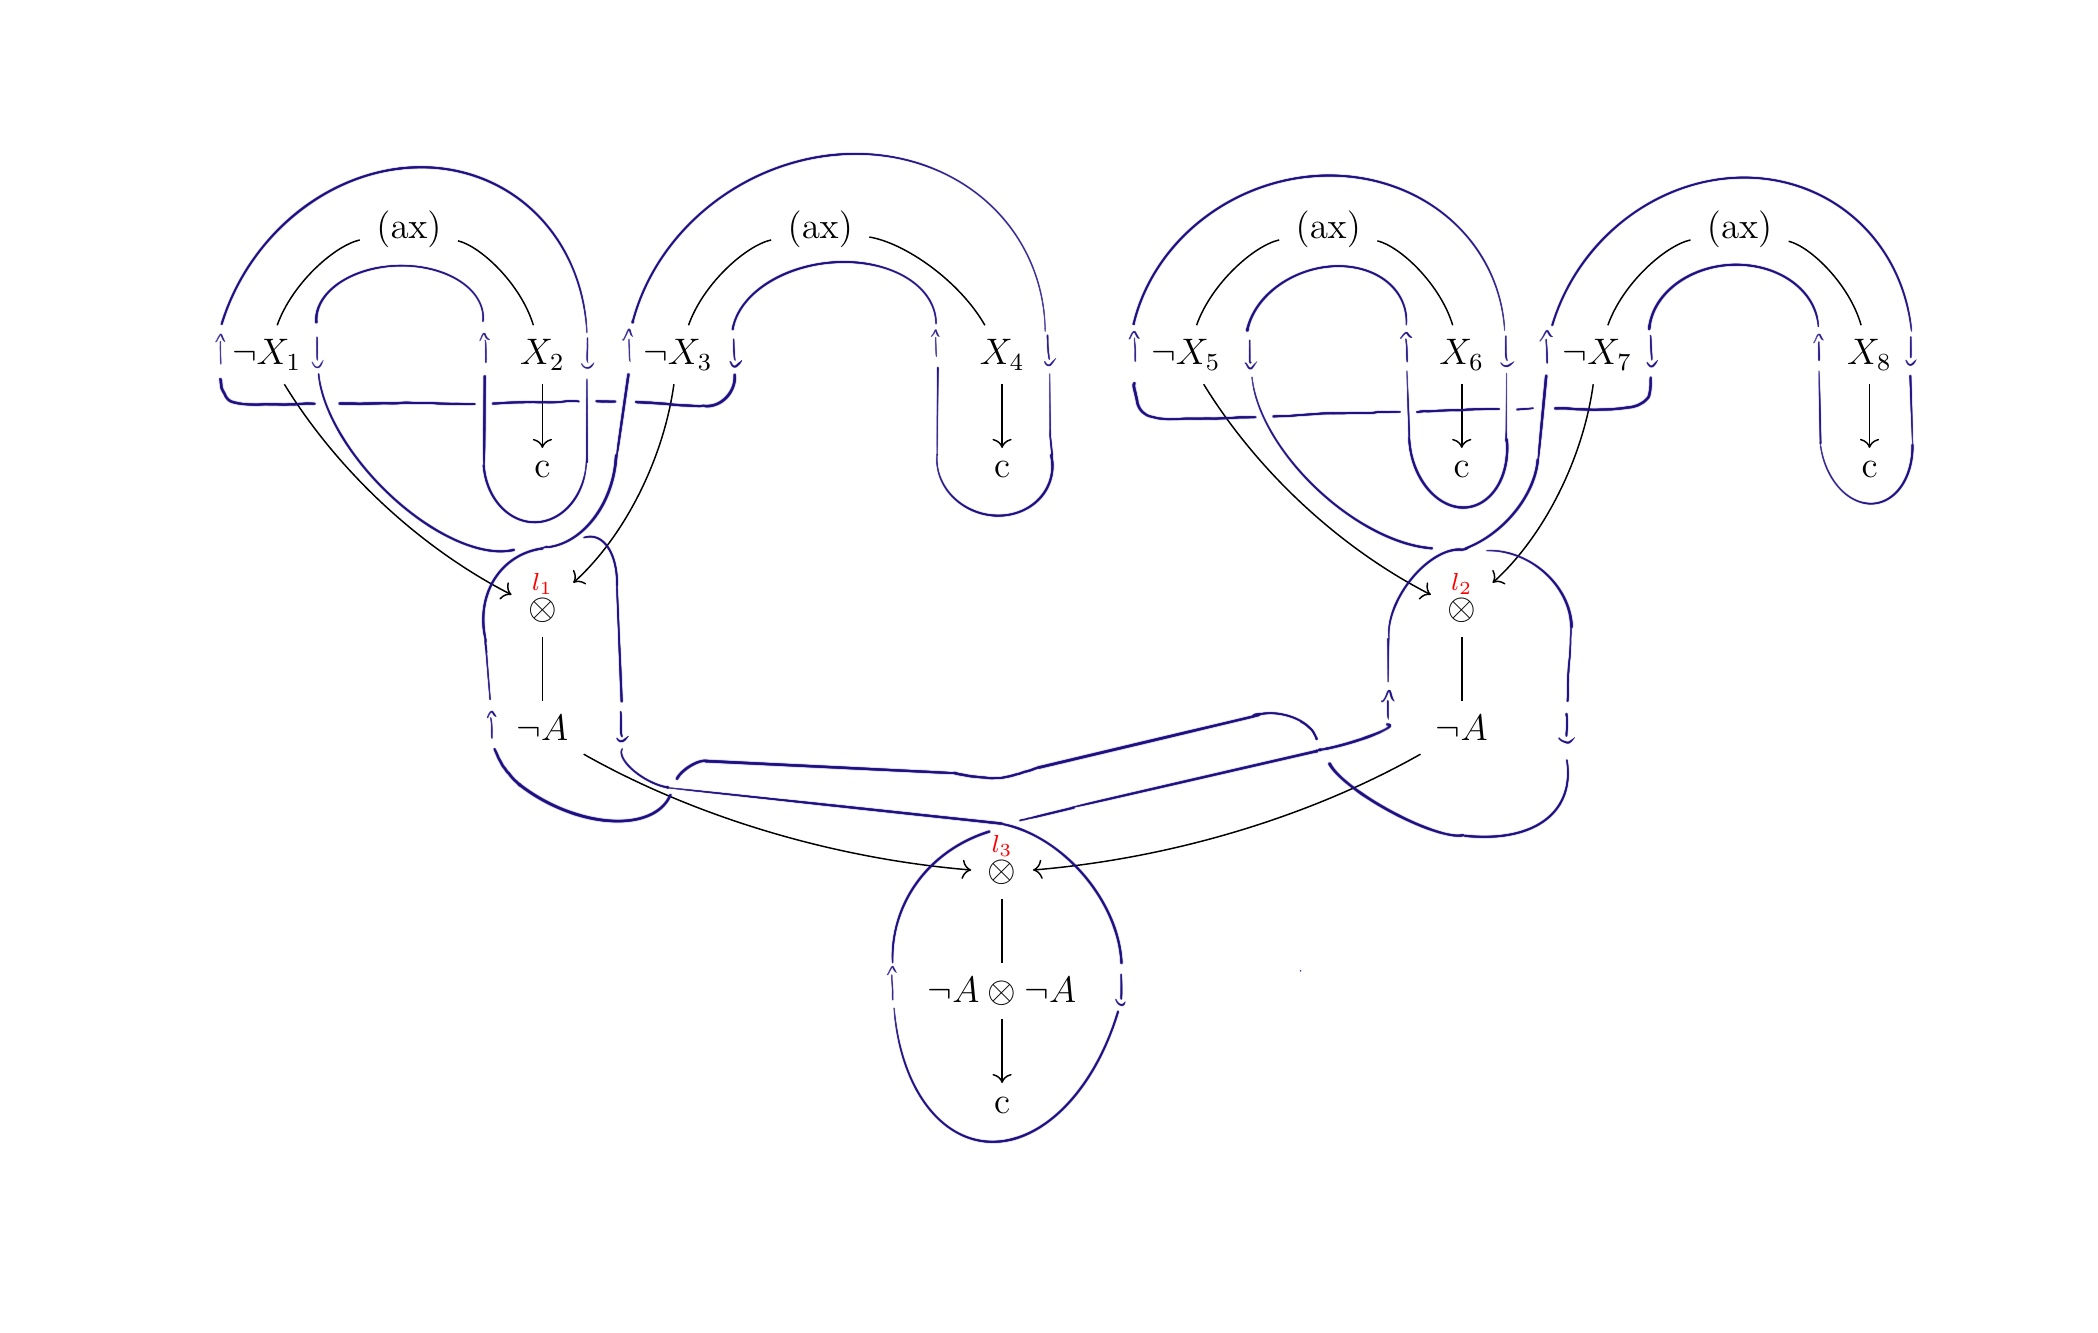
\includegraphics[width = 20cm]{Switching.jpg}
			\caption{The switching $S$ of Example \ref{ex:counter}}
			\label{fig:counter_one}
		\end{figure}
		Let $\pi$ denote the following proof structure with tensor links labelled $l_1, l_2, l_3$ as displayed. The formula $A$ denotes $\neg X \otimes \neg X$.
		% https://q.uiver.app/?q=WzAsMjMsWzAsMSwiXFxuZWcgWF8xIl0sWzIsMSwiWF8yIl0sWzMsMSwiXFxuZWcgWF8zIl0sWzUsMSwiWF80Il0sWzIsMywiXFxvdGltZXMiXSxbMiw0LCJcXG5lZyBBIl0sWzEsMCwiXFxheCJdLFs0LDAsIlxcYXgiXSxbNiwxLCJcXG5lZyBYXzUiXSxbOCwxLCJYXzYiXSxbOSwxLCJcXG5lZyBYXzciXSxbMTEsMSwiWF84Il0sWzEwLDAsIlxcYXgiXSxbNywwLCJcXGF4Il0sWzgsMywiXFxvdGltZXMiXSxbOCw0LCJcXG5lZyBBIl0sWzUsNSwiXFxvdGltZXMiXSxbNSw2LCJcXG5lZyBBIFxcb3RpbWVzIFxcbmVnIEEiXSxbNSw3LCJcXG9wZXJhdG9ybmFtZXtjfSJdLFsyLDIsIlxcb3BlcmF0b3JuYW1le2N9Il0sWzUsMiwiXFxvcGVyYXRvcm5hbWV7Y30iXSxbOCwyLCJcXG9wZXJhdG9ybmFtZXtjfSJdLFsxMSwyLCJcXG9wZXJhdG9ybmFtZXtjfSJdLFswLDQsIiIsMCx7ImN1cnZlIjoyfV0sWzIsNCwiIiwyLHsiY3VydmUiOi0yfV0sWzQsNSwiIiwwLHsic3R5bGUiOnsiaGVhZCI6eyJuYW1lIjoibm9uZSJ9fX1dLFs2LDAsIiIsMCx7ImN1cnZlIjoyLCJzdHlsZSI6eyJoZWFkIjp7Im5hbWUiOiJub25lIn19fV0sWzYsMSwiIiwyLHsiY3VydmUiOi0yLCJzdHlsZSI6eyJoZWFkIjp7Im5hbWUiOiJub25lIn19fV0sWzcsMiwiIiwyLHsiY3VydmUiOjIsInN0eWxlIjp7ImhlYWQiOnsibmFtZSI6Im5vbmUifX19XSxbNywzLCIiLDAseyJjdXJ2ZSI6LTIsInN0eWxlIjp7ImhlYWQiOnsibmFtZSI6Im5vbmUifX19XSxbMTMsOCwiIiwwLHsiY3VydmUiOjIsInN0eWxlIjp7ImhlYWQiOnsibmFtZSI6Im5vbmUifX19XSxbMTMsOSwiIiwyLHsiY3VydmUiOi0yLCJzdHlsZSI6eyJoZWFkIjp7Im5hbWUiOiJub25lIn19fV0sWzEyLDEwLCIiLDIseyJjdXJ2ZSI6Miwic3R5bGUiOnsiaGVhZCI6eyJuYW1lIjoibm9uZSJ9fX1dLFsxMiwxMSwiIiwwLHsiY3VydmUiOi0yLCJzdHlsZSI6eyJoZWFkIjp7Im5hbWUiOiJub25lIn19fV0sWzgsMTQsIiIsMCx7ImN1cnZlIjoyfV0sWzEwLDE0LCIiLDIseyJjdXJ2ZSI6LTJ9XSxbMTQsMTUsIiIsMix7InN0eWxlIjp7ImhlYWQiOnsibmFtZSI6Im5vbmUifX19XSxbNSwxNiwiIiwwLHsiY3VydmUiOjJ9XSxbMTUsMTYsIiIsMix7ImN1cnZlIjotMn1dLFsxNiwxNywiIiwyLHsic3R5bGUiOnsiaGVhZCI6eyJuYW1lIjoibm9uZSJ9fX1dLFsxNywxOF0sWzEsMTldLFszLDIwXSxbOSwyMV0sWzExLDIyXV0=
		\[\begin{tikzcd}[column sep = tiny, row sep = small]
			& \ax &&& \ax &&& \ax &&& \ax \\
			{\neg X_1} && {X_2} & {\neg X_3} && {X_4} & {\neg X_5} && {X_6} & {\neg X_7} && {X_8} \\
			&& {\operatorname{c}} &&& {\operatorname{c}} &&& {\operatorname{c}} &&& {\operatorname{c}} \\
			&& \stackrel{\textcolor{red}{l_1}}{\otimes} &&&&&& \stackrel{\textcolor{red}{l_2}}{\otimes} \\
			&& {\neg A} &&&&&& {\neg A} \\
			&&&&& \stackrel{\textcolor{red}{l_3}}{\otimes} \\
			&&&&& {\neg A \otimes \neg A} \\
			&&&&& {\operatorname{c}}
			\arrow[curve={height=12pt}, from=2-1, to=4-3]
			\arrow[curve={height=-12pt}, from=2-4, to=4-3]
			\arrow[no head, from=4-3, to=5-3]
			\arrow[curve={height=12pt}, no head, from=1-2, to=2-1]
			\arrow[curve={height=-12pt}, no head, from=1-2, to=2-3]
			\arrow[curve={height=12pt}, no head, from=1-5, to=2-4]
			\arrow[curve={height=-12pt}, no head, from=1-5, to=2-6]
			\arrow[curve={height=12pt}, no head, from=1-8, to=2-7]
			\arrow[curve={height=-12pt}, no head, from=1-8, to=2-9]
			\arrow[curve={height=12pt}, no head, from=1-11, to=2-10]
			\arrow[curve={height=-12pt}, no head, from=1-11, to=2-12]
			\arrow[curve={height=12pt}, from=2-7, to=4-9]
			\arrow[curve={height=-12pt}, from=2-10, to=4-9]
			\arrow[no head, from=4-9, to=5-9]
			\arrow[curve={height=12pt}, from=5-3, to=6-6]
			\arrow[curve={height=-12pt}, from=5-9, to=6-6]
			\arrow[no head, from=6-6, to=7-6]
			\arrow[from=7-6, to=8-6]
			\arrow[from=2-3, to=3-3]
			\arrow[from=2-6, to=3-6]
			\arrow[from=2-9, to=3-9]
			\arrow[from=2-12, to=3-12]
		\end{tikzcd}\]
	Consider first the switching $S(l_1) = S(l_2) = S(l_3) = L$. Then we have
	\begin{equation}
		\beta_\pi^S: X_1 \mapsto X_7 \mapsto X_5 \mapsto X_3 \mapsto X_1, \quad X_i \mapsto X_i, i = 2,4,6,8
		\end{equation}
	The other permutations are as follows.
	\begin{align*}
		&X_1 \mapsto X_3 \mapsto X_7 \mapsto X_5 \mapsto X_1, \quad X_i \mapsto X_i, i = 2,4,6,8\\
		&X_1 \mapsto X_3 \mapsto X_5 \mapsto X_7 \mapsto X_1, \quad X_i \mapsto X_i, i = 2,4,6,8\\
		&X_1 \mapsto X_5 \mapsto X_7 \mapsto X_3 \mapsto X_1, \quad X_i \mapsto X_i, i = 2,4,6,8
		\end{align*}
	\end{example}
	We can now rephrase the longtrip condition of Section \ref{sec:sequentialisation} in terms of permutations.
	\begin{proposition}
		Let $\pi$ be a proof structure, then $\pi$ is a proof net if and only if for all $\beta \in \Sigma(\pi)$ the permutation $\alpha_{\pi}\beta$ is cyclic.
	\end{proposition}
	If $\pi$ is a proof net admitting a single conclusion, then it is \emph{not} the case that $\alpha_\pi$ uniquely determines this proof net. For instance, the following pair of proof nets admit the same axiom link permutations, where $C$ denotes $(A \otimes B) \parr (\neg A \parr \neg B)$.
	\[\begin{tikzcd}[column sep = tiny, row sep = small]
		& \ax &&& \ax &&& \ax \\
		{\neg A \parr \neg B} && {A \otimes B} & \neg A && {A} & \neg B && {B } \\
		& \parr &&& \parr && \otimes \\
		& {C} &&& {\neg A \parr \neg B} && {A \otimes B} \\
		& {\operatorname{c}} &&&& \parr \\
		&&&&& {C} \\
		&&&&& {\operatorname{c}}
		\arrow[curve={height=12pt}, no head, from=1-8, to=2-7]
		\arrow[curve={height=-12pt}, no head, from=1-8, to=2-9]
		\arrow[curve={height=12pt}, no head, from=1-5, to=2-4]
		\arrow[curve={height=-12pt}, no head, from=1-5, to=2-6]
		\arrow[curve={height=12pt}, from=2-4, to=3-5]
		\arrow[curve={height=-12pt}, from=2-7, to=3-5]
		\arrow[curve={height=12pt}, from=2-6, to=3-7]
		\arrow[curve={height=-12pt}, from=2-9, to=3-7]
		\arrow[no head, from=3-7, to=4-7]
		\arrow[no head, from=3-5, to=4-5]
		\arrow[curve={height=12pt}, from=4-5, to=5-6]
		\arrow[curve={height=-12pt}, from=4-7, to=5-6]
		\arrow[no head, from=5-6, to=6-6]
		\arrow[from=6-6, to=7-6]
		\arrow[curve={height=12pt}, no head, from=1-2, to=2-1]
		\arrow[curve={height=-12pt}, no head, from=1-2, to=2-3]
		\arrow[curve={height=-12pt}, from=2-3, to=3-2]
		\arrow[curve={height=12pt}, from=2-1, to=3-2]
		\arrow[no head, from=3-2, to=4-2]
		\arrow[from=4-2, to=5-2]
	\end{tikzcd}\]
	\begin{proposition}\label{prop:alpha_uniqueness}
		Let $\pi$ be a cut-free proof net with only one conclusion, assume also that all conclusions of all axiom links are atomic. Then $\pi$ is determined uniquely by $\alpha_\pi$ and the conclusion $A$.
	\end{proposition}
	\begin{proof}
		Let $A$ be the sole conclusion of $\pi$. Consider the typing tree of $A$, this is a binary tree with all leaves labelled by atomic propositions. The proof net $\pi$ is constructed from this by choosing axiom links, this choice of axiom links is determined by $\alpha_\pi$.
	\end{proof}
	\begin{cor}
		Let $\pi$ be a cut-free proof net with conclusions $A_1,...,A_n$, assume also that all conclusions of all axiom links are atomic. Then $\pi$ is determined uniquely by $\alpha_\pi$ and the conclusions $A_1,...,A_n$.
	\end{cor}\label{cor:super_normal_form}
	\begin{proof}
		Let $\pi_1,\pi_2$ be two such proof nets. Construct a new proof net $\pi_1'$ from $\pi_1$ by creating par links (in any order) so that $\pi_1'$ has a unique conclusion $A_1 \parr \hdots \parr A_n$. Construct a new proof net $\pi_2'$ in a similar way and make the same choices of par links made when $\pi_1'$ was constructed. No axiom links were altered in this process, and so $\alpha_{\pi_1} = \alpha_{\pi_1'} = \alpha_{\pi_2'} = \alpha_{\pi_2}$. It follows from Proposition \ref{prop:alpha_uniqueness} that $\pi_1 = \pi_2$.
	\end{proof}
	\begin{example}
		% https://q.uiver.app/?q=WzAsMTUsWzMsNiwiXFxwYXJyIl0sWzEsNSwiQSBcXG90aW1lcyBBIl0sWzUsNSwiXFxuZWcgQSBcXHBhcnIgXFxuZWcgQSJdLFs0LDMsIlxcbmVnIEEiXSxbNiwzLCJcXG5lZyBBIl0sWzIsMywiQSJdLFswLDMsIkEiXSxbNSw0LCJcXHBhcnIiXSxbMSw0LCJcXG90aW1lcyJdLFszLDEsIlxcYXgiXSxbMywwLCJcXGF4Il0sWzQsMiwiXFxheCJdLFsyLDIsIlxcYXgiXSxbMyw3LCIoQSBcXG90aW1lcyBBKSBcXHBhcnIgKFxcbmVnIEEgXFxwYXJyIFxcbmVnIEEpIl0sWzMsOCwiXFxvcGVyYXRvcm5hbWV7Y30iXSxbMSwwLCIiLDAseyJjdXJ2ZSI6Mn1dLFsyLDAsIiIsMix7ImN1cnZlIjotMn1dLFs0LDddLFszLDddLFs3LDIsIiIsMCx7InN0eWxlIjp7ImhlYWQiOnsibmFtZSI6Im5vbmUifX19XSxbNSw4XSxbNiw4XSxbOCwxLCIiLDIseyJzdHlsZSI6eyJoZWFkIjp7Im5hbWUiOiJub25lIn19fV0sWzksMywiIiwwLHsiY3VydmUiOi0xLCJzdHlsZSI6eyJib2R5Ijp7Im5hbWUiOiJkYXNoZWQifSwiaGVhZCI6eyJuYW1lIjoibm9uZSJ9fX1dLFs5LDUsIiIsMSx7ImN1cnZlIjoxLCJzdHlsZSI6eyJib2R5Ijp7Im5hbWUiOiJkYXNoZWQifSwiaGVhZCI6eyJuYW1lIjoibm9uZSJ9fX1dLFsxMCw0LCIiLDIseyJjdXJ2ZSI6LTMsInN0eWxlIjp7ImJvZHkiOnsibmFtZSI6ImRhc2hlZCJ9LCJoZWFkIjp7Im5hbWUiOiJub25lIn19fV0sWzEwLDYsIiIsMSx7ImN1cnZlIjozLCJzdHlsZSI6eyJib2R5Ijp7Im5hbWUiOiJkYXNoZWQifSwiaGVhZCI6eyJuYW1lIjoibm9uZSJ9fX1dLFsxMSw0LCIiLDEseyJjdXJ2ZSI6LTEsInN0eWxlIjp7ImhlYWQiOnsibmFtZSI6Im5vbmUifX19XSxbMTEsNSwiIiwxLHsiY3VydmUiOjMsInN0eWxlIjp7ImhlYWQiOnsibmFtZSI6Im5vbmUifX19XSxbMTIsNiwiIiwxLHsiY3VydmUiOjEsInN0eWxlIjp7ImhlYWQiOnsibmFtZSI6Im5vbmUifX19XSxbMTIsMywiIiwxLHsiY3VydmUiOi0zLCJzdHlsZSI6eyJoZWFkIjp7Im5hbWUiOiJub25lIn19fV0sWzAsMTMsIiIsMCx7InN0eWxlIjp7ImhlYWQiOnsibmFtZSI6Im5vbmUifX19XSxbMTMsMTRdXQ==
		\begin{equation}\label{eq:counter_one}
			\begin{tikzcd}[column sep = tiny, row sep = small]
				&&& \ax \\
				&&& \ax \\
				&& \ax && \ax \\
				X_1 && X_2 && {\neg X_3} && {\neg X_4} \\
				& \otimes &&&& \parr \\
				& {X \otimes X} &&&& {\neg X\parr \neg X} \\
				&&& \parr \\
				&&& {(X\otimes X) \parr (\neg X \parr \neg X)} \\
				&&& {\operatorname{c}}
				\arrow[curve={height=12pt}, from=6-2, to=7-4]
				\arrow[curve={height=-12pt}, from=6-6, to=7-4]
				\arrow[from=4-7, to=5-6]
				\arrow[from=4-5, to=5-6]
				\arrow[no head, from=5-6, to=6-6]
				\arrow[from=4-3, to=5-2]
				\arrow[from=4-1, to=5-2]
				\arrow[no head, from=5-2, to=6-2]
				\arrow[curve={height=-6pt}, dashed, no head, from=2-4, to=4-5]
				\arrow[curve={height=6pt}, dashed, no head, from=2-4, to=4-3]
				\arrow[curve={height=-18pt}, dashed, no head, from=1-4, to=4-7]
				\arrow[curve={height=18pt}, dashed, no head, from=1-4, to=4-1]
				\arrow[curve={height=-6pt}, no head, from=3-5, to=4-7]
				\arrow[curve={height=18pt}, no head, from=3-5, to=4-3]
				\arrow[curve={height=6pt}, no head, from=3-3, to=4-1]
				\arrow[curve={height=-18pt}, no head, from=3-3, to=4-5]
				\arrow[no head, from=7-4, to=8-4]
				\arrow[from=8-4, to=9-4]
			\end{tikzcd}
		\end{equation}
		The proof net given by ignoring the dashed lines in \eqref{eq:counter_one} corresponds to the permutation
		\begin{equation}
			X_1 \leftrightarrow X_2, X_3 \leftrightarrow X_4
			\end{equation}
		and that given by ignoring the axiom links and including the dashed lines is
		\begin{equation}
			X_1 \leftrightarrow X_4, X_2 \leftrightarrow X_3
			\end{equation}
	\end{example}
	
	\subsection{Geometry of Interaction Zero}\label{sec:goi_zero}
	We begin with the following crucial observation:
	\begin{lemma}\label{lem:GoI_lemma}
		Let $\pi$ be a proof structure such that every conclusion of every atom link is atomic. Assume there is a cut in $\pi$ with premises $A, \neg A$. Write
		\begin{equation}
			A :=  X_1 \boxtimes_1 \hdots \boxtimes_{n-1} X_n
		\end{equation}
		where for each $i = 1,\ldots, n-1$ we have $\boxtimes_i \in \lbrace \otimes, \parr\rbrace$ and for each $i = 1,\ldots,n$ we have that $X_i$ is atomic. Let $\zeta$ be a proof structure equivalent to $\pi$ under cut-reduction which is obtained by reducing all $m$-redexes (Definition \ref{def:reduction}). Then in $\zeta$, there exists for each $i$ a cut link $l_i$ with premises $X_i, \neg X_i$.
	\end{lemma}
	\begin{proof}
		By induction on $n$, where the base case follows trivially and the inductive step by inspection of \eqref{rule:tensor_reduct}.
	\end{proof}
Using Lemma \ref{lem:GoI_lemma}, if $\pi$ is a cut-free proof structure with all conclusions to all axiom links atomic, then we can identify the atoms in the premises of the cut links with the atoms in the conclusions of the axiom links. We will do this throughout this section.
	\begin{defn}\label{def:perm_cut}
		We define a permutation $\gamma_\pi$ on $\call{P}(\pi)$ (Definition \ref{def:atomic_atoms_ax_concs}). Let $l$ be a cut link in $\pi$ with premises $\neg A, A$, say. Let $\neg A,A$ have corresponding unoriented atoms $X_1,\ldots, X_n$ and  $Y_1,\ldots, Y_n$. Let $\gamma_l$ be the permutation which swaps $X_j$ and $Y_j$. Ranging over all cut links $l_1,\ldots, l_n$ we define
		\begin{equation}
			\gamma_\pi := \gamma_{l_1}\ldots \gamma_{l_n}
			\end{equation}
	\end{defn}
	\begin{example}
		We denote by $\pi$ the following proof net with artificial labels on the formulas. Assume $X_i$ for $i = 1,\ldots, 6$ is atomic.
		% https://q.uiver.app/?q=WzAsMTYsWzAsMSwiQSJdLFsxLDAsIlxcYXgiXSxbMiwxLCJcXG5lZyBBIl0sWzMsMiwiXFxvdGltZXMiXSxbNCwxLCJBIl0sWzYsMSwiXFxuZWcgQSJdLFs1LDAsIlxcYXgiXSxbMywzLCJcXG5lZyBBIFxcb3RpbWVzIEEiXSxbNywxLCJBIl0sWzgsMCwiXFxheCJdLFs5LDEsIlxcbmVnIEEiXSxbOCwyLCJcXHBhcnIiXSxbOCwzLCJBIFxccGFyciBcXG5lZyBBIl0sWzYsNCwiXFxjdXQiXSxbNiwyLCJcXG9wZXJhdG9ybmFtZXtjfSJdLFswLDIsIlxcb3BlcmF0b3JuYW1le2N9Il0sWzEsMCwiIiwwLHsiY3VydmUiOjIsInN0eWxlIjp7ImhlYWQiOnsibmFtZSI6Im5vbmUifX19XSxbMSwyLCIiLDIseyJjdXJ2ZSI6LTIsInN0eWxlIjp7ImhlYWQiOnsibmFtZSI6Im5vbmUifX19XSxbNiw0LCIiLDIseyJjdXJ2ZSI6Miwic3R5bGUiOnsiaGVhZCI6eyJuYW1lIjoibm9uZSJ9fX1dLFs2LDUsIiIsMCx7ImN1cnZlIjotMiwic3R5bGUiOnsiaGVhZCI6eyJuYW1lIjoibm9uZSJ9fX1dLFs0LDMsIiIsMix7ImN1cnZlIjotMn1dLFsyLDMsIiIsMSx7ImN1cnZlIjoyfV0sWzMsNywiIiwxLHsic3R5bGUiOnsiaGVhZCI6eyJuYW1lIjoibm9uZSJ9fX1dLFs5LDgsIiIsMSx7ImN1cnZlIjoyLCJzdHlsZSI6eyJoZWFkIjp7Im5hbWUiOiJub25lIn19fV0sWzksMTAsIiIsMSx7ImN1cnZlIjotMiwic3R5bGUiOnsiaGVhZCI6eyJuYW1lIjoibm9uZSJ9fX1dLFs4LDExLCIiLDEseyJjdXJ2ZSI6Mn1dLFsxMCwxMSwiIiwxLHsiY3VydmUiOi0yfV0sWzExLDEyLCIiLDEseyJzdHlsZSI6eyJoZWFkIjp7Im5hbWUiOiJub25lIn19fV0sWzcsMTMsIiIsMSx7ImN1cnZlIjoyfV0sWzEyLDEzLCIiLDEseyJjdXJ2ZSI6LTJ9XSxbMCwxNV0sWzUsMTRdXQ==
		\begin{equation}\label{eq:standard_example}
			\begin{tikzcd}[column sep = small, row sep = small]
				& \ax &&&& \ax &&& \ax \\
				\neg X_1 && {X_2} && \neg X_3 && {X_4} & \neg X_5 && {X_6} \\
				{\operatorname{c}} &&& \otimes &&& {\operatorname{c}} && \parr \\
				&&& {X \otimes \neg X} &&&&& {\neg X \parr X} \\
				&&&&&& \cut
				\arrow[curve={height=12pt}, no head, from=1-2, to=2-1]
				\arrow[curve={height=-12pt}, no head, from=1-2, to=2-3]
				\arrow[curve={height=12pt}, no head, from=1-6, to=2-5]
				\arrow[curve={height=-12pt}, no head, from=1-6, to=2-7]
				\arrow[curve={height=-12pt}, from=2-5, to=3-4]
				\arrow[curve={height=12pt}, from=2-3, to=3-4]
				\arrow[no head, from=3-4, to=4-4]
				\arrow[curve={height=12pt}, no head, from=1-9, to=2-8]
				\arrow[curve={height=-12pt}, no head, from=1-9, to=2-10]
				\arrow[curve={height=12pt}, from=2-8, to=3-9]
				\arrow[curve={height=-12pt}, from=2-10, to=3-9]
				\arrow[no head, from=3-9, to=4-9]
				\arrow[curve={height=12pt}, from=4-4, to=5-7]
				\arrow[curve={height=-12pt}, from=4-9, to=5-7]
				\arrow[from=2-1, to=3-1]
				\arrow[from=2-7, to=3-7]
			\end{tikzcd}
		\end{equation}
		We have
		\begin{equation}
			\gamma_\pi: X_2 \leftrightarrow X_5,\quad X_3 \leftrightarrow X_6,\quad X_i \leftrightarrow X_i, i = 1,4
			\end{equation}
	\end{example}

	\begin{lemma}\label{lem:particular_redex_form}
		The set $\call{P}(\pi)$ is invariant under reduction of $m$-redexes and $\eta$-expansion. More precisely, we have the following two statements.
		\begin{itemize}
			\item Say $\pi'$ is produced by reducing an $m$-redex \eqref{rule:tensor_reduct} in $\pi$, then $\call{P}(\pi) = \call{P}(\pi')$.
			\item Say $\pi \lto_\eta \pi'$ (see Definition \ref{def:eta_expansion}), then $\call{P}(\pi) = \call{P}(\pi')$.
		\end{itemize}
	\end{lemma}
	\begin{proof}
		For the first claim we simply notice that rule \eqref{rule:tensor_reduct} has no effect on the axiom links of $\pi$. For the second we see that the order of the sequence of unoriented atoms of $A,B$ is explicated by the axiom links produced by an $\eta$-expansion.
	\end{proof}
	Hence, when considering $\call{P}(\pi)$, we can always assume without loss of generality that $\pi$ contains no $m$-redexes and that all conclusions of all axiom links of $\pi$ are atomic.
	\begin{lemma}\label{lem:redexes_particular_form}
		Let $\pi$ be a proof net admitting no $m$-redexes and assume that all conclusions of all axiom links of $\pi$ are atomic. All redexes $\pi \lto_{\cut} \pi'$ are necessarily of the following form, with $X$ atomic.
		% https://q.uiver.app/?q=WzAsMTQsWzEsMCwiXFxheCJdLFswLDEsIlgiXSxbMiwxLCJcXG5lZyBYIl0sWzMsMiwiXFxjdXQiXSxbNCwxLCJYIl0sWzUsMCwiXFxheCJdLFs2LDEsIlxcbmVnIFgiXSxbOSwwLCJcXGF4Il0sWzgsMSwiWCJdLFsxMCwxLCJcXG5lZyBYIl0sWzAsMiwiXFx2ZG90cyJdLFs2LDIsIlxcdmRvdHMiXSxbOCwyLCJcXHZkb3RzIl0sWzEwLDIsIlxcdmRvdHMiXSxbMCwxLCIiLDAseyJjdXJ2ZSI6Miwic3R5bGUiOnsiaGVhZCI6eyJuYW1lIjoibm9uZSJ9fX1dLFswLDIsIiIsMix7ImN1cnZlIjotMiwic3R5bGUiOnsiaGVhZCI6eyJuYW1lIjoibm9uZSJ9fX1dLFsxLDEwXSxbMiwzLCIiLDIseyJjdXJ2ZSI6Mn1dLFs0LDMsIiIsMCx7ImN1cnZlIjotMn1dLFs1LDQsIiIsMCx7ImN1cnZlIjoyLCJzdHlsZSI6eyJoZWFkIjp7Im5hbWUiOiJub25lIn19fV0sWzUsNiwiIiwyLHsiY3VydmUiOi0yLCJzdHlsZSI6eyJoZWFkIjp7Im5hbWUiOiJub25lIn19fV0sWzYsMTFdLFs3LDgsIiIsMix7ImN1cnZlIjoyLCJzdHlsZSI6eyJoZWFkIjp7Im5hbWUiOiJub25lIn19fV0sWzcsOSwiIiwwLHsiY3VydmUiOi0yLCJzdHlsZSI6eyJoZWFkIjp7Im5hbWUiOiJub25lIn19fV0sWzksMTNdLFs4LDEyXV0=
		\begin{equation}\label{eq:redex_form}
			\begin{tikzcd}[column sep = small, row sep = small]
				& \ax &&&& \ax &&&& \ax \\
				\neg X && {X} && \neg X && {X} && \neg X && {X} \\
				\vdots &&& \cut &&& \vdots && \vdots && \vdots
				\arrow[curve={height=12pt}, no head, from=1-2, to=2-1]
				\arrow[curve={height=-12pt}, no head, from=1-2, to=2-3]
				\arrow[from=2-1, to=3-1]
				\arrow[curve={height=12pt}, from=2-3, to=3-4]
				\arrow[curve={height=-12pt}, from=2-5, to=3-4]
				\arrow[curve={height=12pt}, no head, from=1-6, to=2-5]
				\arrow[curve={height=-12pt}, no head, from=1-6, to=2-7]
				\arrow[from=2-7, to=3-7]
				\arrow[curve={height=12pt}, no head, from=1-10, to=2-9]
				\arrow[curve={height=-12pt}, no head, from=1-10, to=2-11]
				\arrow[from=2-11, to=3-11]
				\arrow[from=2-9, to=3-9]
			\end{tikzcd}
		\end{equation}
	\end{lemma}
	\begin{proof}
		All redexes of $\pi$ are $a$-redexes, so all redexes of $\pi$ are of the form \eqref{rule:ax_reduct_negation} or \eqref{rule:ax_reduct}, but since all the axiom links have atoms as conclusions, it must be the case that the cut link in \eqref{rule:ax_reduct_negation}, \eqref{rule:ax_reduct} have premises which are also atoms. These atoms can only possibly exist if they are conclusions to an axiom link, and so we obtain the form given in the statement.
	\end{proof}
	\begin{defn}\label{def:injective_function}
		Say $\pi$ is a proof net with no $m$-redexes and all conclusions of all axiom links are atomic. Moreover, say there is a reduction $\pi \lto \pi'$ which by Lemma \ref{lem:particular_redex_form} is of the form \eqref{eq:redex_form}. We define a function $\iota: \call{P}(\pi') \rightarrowtail \call{P}(\pi)$ given by the following schema:
		% https://q.uiver.app/?q=WzAsMTQsWzEsMywiXFxheCJdLFswLDQsIkEiXSxbMiw0LCJcXG5lZyBBIl0sWzMsNSwiXFxjdXQiXSxbNCw0LCJBIl0sWzAsNSwiXFx2ZG90cyJdLFs1LDMsIlxcYXgiXSxbNiw0LCJcXG5lZyBBIl0sWzYsNSwiXFx2ZG90cyJdLFsyLDEsIkEiXSxbNCwxLCJcXG5lZyBBIl0sWzMsMCwiXFxheCJdLFsyLDIsIlxcdmRvdHMiXSxbNCwyLCJcXHZkb3RzIl0sWzAsMSwiIiwwLHsiY3VydmUiOjIsInN0eWxlIjp7ImhlYWQiOnsibmFtZSI6Im5vbmUifX19XSxbMCwyLCIiLDIseyJjdXJ2ZSI6LTIsInN0eWxlIjp7ImhlYWQiOnsibmFtZSI6Im5vbmUifX19XSxbMiwzLCIiLDIseyJjdXJ2ZSI6Mn1dLFs0LDMsIiIsMCx7ImN1cnZlIjotMn1dLFsxLDVdLFs2LDQsIiIsMCx7ImN1cnZlIjoyLCJzdHlsZSI6eyJoZWFkIjp7Im5hbWUiOiJub25lIn19fV0sWzYsNywiIiwyLHsiY3VydmUiOi0yLCJzdHlsZSI6eyJoZWFkIjp7Im5hbWUiOiJub25lIn19fV0sWzcsOF0sWzExLDksIiIsMix7ImN1cnZlIjoyLCJzdHlsZSI6eyJoZWFkIjp7Im5hbWUiOiJub25lIn19fV0sWzExLDEwLCIiLDAseyJjdXJ2ZSI6LTIsInN0eWxlIjp7ImhlYWQiOnsibmFtZSI6Im5vbmUifX19XSxbMTAsMTNdLFs5LDEyXSxbOSwxLCIiLDEseyJjdXJ2ZSI6NSwiY29sb3VyIjpbMzAwLDYwLDYwXX1dLFsxMCw3LCIiLDEseyJjdXJ2ZSI6LTUsImNvbG91ciI6WzMwMCw2MCw2MF19XV0=
		\begin{equation}\label{eq:inclusion_definition}
		\begin{tikzcd}[column sep = small, row sep = small]
			&&& \ax \\
			&& \neg X && {X} \\
			&& \vdots && \vdots \\
			& \ax &&&& \ax \\
			\neg X && {X} && \neg X && {X} \\
			\vdots &&& \cut &&& \vdots
			\arrow[curve={height=12pt}, no head, from=4-2, to=5-1]
			\arrow[curve={height=-12pt}, no head, from=4-2, to=5-3]
			\arrow[curve={height=12pt}, from=5-3, to=6-4]
			\arrow[curve={height=-12pt}, from=5-5, to=6-4]
			\arrow[from=5-1, to=6-1]
			\arrow[curve={height=12pt}, no head, from=4-6, to=5-5]
			\arrow[curve={height=-12pt}, no head, from=4-6, to=5-7]
			\arrow[from=5-7, to=6-7]
			\arrow[curve={height=12pt}, no head, from=1-4, to=2-3]
			\arrow[curve={height=-12pt}, no head, from=1-4, to=2-5]
			\arrow[from=2-5, to=3-5]
			\arrow[from=2-3, to=3-3]
			\arrow[color={rgb,255:red,214;green,92;blue,214}, curve={height=30pt}, from=2-3, to=5-1]
			\arrow[color={rgb,255:red,214;green,92;blue,214}, curve={height=-30pt}, from=2-5, to=5-7]
		\end{tikzcd}
\end{equation}
	\end{defn}
	\begin{defn}\label{def:snf_function}
		Let $\pi$ be a proof net and consider $\call{P}(\pi)$, in light of Lemma \ref{lem:particular_redex_form} we can assume without loss of generality that $\pi$ admits no $m$-redexes and that all conclusions of all axiom links in $\pi$ are atomic. Let $\zeta$ be the corresponding super normal form established by Corollary \ref{cor:super_normal_form}. Let $(\pi = \pi_1,\hdots, \pi_n = \zeta)$ be a sequence of cut reductions. These induce a family of functions:
		\begin{equation}
			\call{P}(\zeta) = \call{P}(\pi_n) \rightarrowtail \call{P}(\pi_{n-1}) \lto \hdots \lto \call{P}(\pi_2) \lto \call{P}(\pi_1) = \call{P}(\pi)
		\end{equation}
		Composing these determines a function $\iota_{\pi}: \call{P}(\zeta) \rightarrowtail \call{P}(\pi)$.
	\end{defn}
	\begin{remark}
		It follows from Proposition \ref{prop:church_rosser} that the function $\iota_\pi$ is independent of the choice of reduction path used to define it.
		\end{remark}
	We give an alternate characterisation of the image of $\iota_\pi$.
	\begin{lemma}\label{lem:essence_classification}
		Let $\pi$ be a proof net admitting no $m$-redexes and assume all conclusions of all axiom links are atomic. A formula $A$ in $\pi$ is in $\operatorname{im}\iota_\pi$ if and only if it is \emph{not} premise to a cut link and is the conclusion to an axiom link.
	\end{lemma}
\begin{proof}
	Say $A$ is premise to a cut link. Since $A \in \call{P}(\pi)$ it is also the case that $A$ is conclusion to a cut link. Hence there exists a cut reduction which removes $A$, and so $A$ is not in the image of $\iota_\pi$.
	
	Now say $A$ is \emph{not} premise to a cut link and so $A$ is necessarily \emph{not} part of an $a$-redex. There are no $m$-redexes in $\pi$ and so all cut reductions reduce $a$-redexes. Hence $A$ survives the cut reduction process. In other words, $A \in \operatorname{im}\iota_\pi$.
\end{proof}

\begin{cor}
	Let $\pi$ be a proof net and assume all conclusions of all axiom links are atomic. A formula $A$ in $\pi$ is in $\operatorname{im}\iota_\pi$ if an only if the unique maximal length directed path in $\pi$ starting at the edge labelled $A$ ends at the premise to a cut link.
	\end{cor}
	
	\begin{defn}\label{def:GoI_permutation}
		Let $\pi$ be a proof net. We describe a final permutation $\delta_\pi$ on $\call{P}(\pi)$. Recall the injective function $\iota_\pi$ of Definition \ref{def:snf_function}. For each $X \in \call{P}(\pi)$ let $d_i$ denote the least integer such that 
		\begin{equation}
			(\alpha_{\pi} \circ \gamma_{\pi})^{d_i}(X) \in \operatorname{im}\iota_\pi
		\end{equation}
		Notice that such an integer $d_i$ always exists as $\pi$ is a proof net (as $\pi$ satisfies the longtrip condition, see Section \ref{sec:sequentialisation}).
		
		We then define the following permutation on $\call{P}(\pi)$, the permutations $\alpha_\pi, \gamma_\pi$ Definition \ref{def:permutations}, \ref{def:perm_cut} respectively:
		\begin{equation}
			\delta_{\pi}(X) = (\alpha_\pi \circ \gamma_\pi)^{d_i}(X)
		\end{equation}
	\end{defn}
	\begin{thm}\label{thm:geometry_of_interaction_zero}[Geometry of Interaction zero]
		Let $\pi$ be a proof net possibly with cuts and let $\zeta$ be the normal form of $\pi$ (Definition \ref{def:normal_form}). Then
		\begin{equation}
			\delta_\pi = \iota_{\pi}\alpha_{\zeta}
		\end{equation}
	\end{thm}
	\begin{proof}
		By inspection of \eqref{rule:tensor_reduct} we have that $\gamma_{\pi}$ is invariant under reduction of $m$-redexes. Also, $\alpha_\pi$ is clearly invariant under reduction of $m$-redexes, thus we can assume that $\pi$ admits no $m$-redex. Furthermore, by inspection of \eqref{eq:eta_expansion} we see that $\alpha_\pi$ is invariant under $\eta$-expansion, it is also clear that $\gamma_\pi$ is invariant under $\eta$-expansion. Thus we can also assume that all conclusions of all axiom links of $\pi$ are atomic.
		
		All cut links appear inside ``chains" of axiom and cut links, such as in the following Diagram.
		% https://q.uiver.app/?q=WzAsMTQsWzEsMCwiXFxheCJdLFswLDEsIlgiXSxbMiwxLCJcXG5lZyBYIl0sWzMsMiwiXFxjdXQiXSxbNCwxLCJYIl0sWzUsMCwiXFxoZG90cyJdLFs2LDBdLFs2LDEsIlgiXSxbNywyLCJcXGN1dCJdLFs4LDEsIlxcbmVnIFgiXSxbOSwwLCJcXGF4Il0sWzEwLDEsIlgiXSxbMCwyLCJcXHZkb3RzIl0sWzEwLDIsIlxcdmRvdHMiXSxbMTAsMTEsIiIsMCx7ImN1cnZlIjotMiwic3R5bGUiOnsiaGVhZCI6eyJuYW1lIjoibm9uZSJ9fX1dLFsxMCw5LCIiLDIseyJjdXJ2ZSI6Miwic3R5bGUiOnsiaGVhZCI6eyJuYW1lIjoibm9uZSJ9fX1dLFs5LDgsIiIsMix7ImN1cnZlIjotMn1dLFs3LDgsIiIsMCx7ImN1cnZlIjoyfV0sWzUsNywiIiwwLHsiY3VydmUiOi0yLCJzdHlsZSI6eyJoZWFkIjp7Im5hbWUiOiJub25lIn19fV0sWzUsNCwiIiwyLHsiY3VydmUiOjIsInN0eWxlIjp7ImhlYWQiOnsibmFtZSI6Im5vbmUifX19XSxbNCwzLCIiLDIseyJjdXJ2ZSI6LTJ9XSxbMiwzLCIiLDAseyJjdXJ2ZSI6Mn1dLFswLDIsIiIsMCx7ImN1cnZlIjotMiwic3R5bGUiOnsiaGVhZCI6eyJuYW1lIjoibm9uZSJ9fX1dLFswLDEsIiIsMix7ImN1cnZlIjoyfV0sWzEsMTJdLFsxMSwxM11d
		\[\begin{tikzcd}[column sep = tiny, row sep = small]
			& \ax &&&& \hdots & {} &&& \ax \\
			\neg X && {X} && \neg X && X && {\neg X} && X \\
			\vdots &&& \cut &&&& \cut &&& \vdots
			\arrow[curve={height=-12pt}, no head, from=1-10, to=2-11]
			\arrow[curve={height=12pt}, no head, from=1-10, to=2-9]
			\arrow[curve={height=-12pt}, from=2-9, to=3-8]
			\arrow[curve={height=12pt}, from=2-7, to=3-8]
			\arrow[curve={height=-12pt}, no head, from=1-6, to=2-7]
			\arrow[curve={height=12pt}, no head, from=1-6, to=2-5]
			\arrow[curve={height=-12pt}, from=2-5, to=3-4]
			\arrow[curve={height=12pt}, from=2-3, to=3-4]
			\arrow[curve={height=-12pt}, no head, from=1-2, to=2-3]
			\arrow[curve={height=12pt}, from=1-2, to=2-1]
			\arrow[from=2-1, to=3-1]
			\arrow[from=2-11, to=3-11]
		\end{tikzcd}\]
	By Lemma \ref{lem:essence_classification}, all formulas in the ``interior" of these chains are not in $\operatorname{im}\iota_\pi$. Hence, $\delta_\pi$ is a product of transposes where the formulas on the two extreme ends of these chains are swapped. By considering the cut elimination rules \eqref{rule:ax_reduct_negation}, \eqref{rule:ax_reduct} we see that this is exactly the behaviour of $\alpha_{\zeta}$, and the that these two formulas are the images of the corresponding formulas in $\zeta$.
	\end{proof}

In \cite[Proposition A.1]{AlgPnt} the relationship between the permutation $\delta$ of Definition \ref{def:GoI_permutation} and another permutation coming from the model of Multiplicative Linear Logic as coordinate rings presented there. Here, we show a detailed example of this connection.
\begin{example}
	Let $\pi$ denote the following proof net, we let $(X,+)$ be atomic and denote it by $X$, the formula $C$ denotes $(\neg X \parr  X) \otimes (X \otimes \neg X)$. For convenience, we have artificially labelled the atomic propositions, but throughout, for any $i$ the notation $X_i$ means $X$.
	% https://q.uiver.app/?q=WzAsMTcsWzQsMiwiXFxuZWcgWF81IFxccGFyciBYXzYiXSxbNSwzLCJcXG90aW1lcyJdLFs1LDQsIkMiXSxbNiwyLCJYXzcgXFxvdGltZXMgXFxuZWcgWF84Il0sWzcsMiwiWF85IFxcb3RpbWVzIFxcbmVnIFhfezEwfSJdLFs5LDIsIlxcbmVnIFhfezExfSBcXHBhcnIgWF97MTJ9Il0sWzgsMSwiXFxheCJdLFs4LDMsIlxccGFyciJdLFs4LDQsIlxcbmVnIEMiXSxbNyw1LCJcXGN1dCJdLFszLDEsIlxcYXgiXSxbMiwyLCJYXzMgXFxvdGltZXMgXFxuZWcgWF80Il0sWzMsMCwiXFxheCJdLFswLDIsIlxcbmVnIFhfMSBcXHBhcnIgWF8yIl0sWzEsMywiXFxwYXJyIl0sWzEsNCwiXFxuZWcgQyJdLFsxLDUsIlxcb3BlcmF0b3JuYW1le2N9Il0sWzMsMSwiIiwwLHsiY3VydmUiOi0yfV0sWzAsMSwiIiwxLHsiY3VydmUiOjJ9XSxbMSwyLCIiLDEseyJzdHlsZSI6eyJoZWFkIjp7Im5hbWUiOiJub25lIn19fV0sWzYsNCwiIiwxLHsiY3VydmUiOjIsInN0eWxlIjp7ImhlYWQiOnsibmFtZSI6Im5vbmUifX19XSxbNiw1LCIiLDEseyJjdXJ2ZSI6LTIsInN0eWxlIjp7ImhlYWQiOnsibmFtZSI6Im5vbmUifX19XSxbNCw3LCIiLDEseyJjdXJ2ZSI6Mn1dLFs1LDcsIiIsMSx7ImN1cnZlIjotMn1dLFs3LDgsIiIsMSx7InN0eWxlIjp7ImhlYWQiOnsibmFtZSI6Im5vbmUifX19XSxbMiw5LCIiLDEseyJjdXJ2ZSI6Mn1dLFs4LDksIiIsMSx7ImN1cnZlIjotMn1dLFsxMCwwLCIiLDEseyJjdXJ2ZSI6LTIsInN0eWxlIjp7ImhlYWQiOnsibmFtZSI6Im5vbmUifX19XSxbMTAsMTEsIiIsMSx7ImN1cnZlIjoyLCJzdHlsZSI6eyJoZWFkIjp7Im5hbWUiOiJub25lIn19fV0sWzEyLDMsIiIsMix7ImN1cnZlIjotMywic3R5bGUiOnsiaGVhZCI6eyJuYW1lIjoibm9uZSJ9fX1dLFsxMiwxMywiIiwwLHsiY3VydmUiOjMsInN0eWxlIjp7ImhlYWQiOnsibmFtZSI6Im5vbmUifX19XSxbMTEsMTQsIiIsMCx7ImN1cnZlIjotMn1dLFsxMywxNCwiIiwxLHsiY3VydmUiOjF9XSxbMTQsMTUsIiIsMSx7InN0eWxlIjp7ImhlYWQiOnsibmFtZSI6Im5vbmUifX19XSxbMTUsMTZdXQ==
	\[\begin{tikzcd}[column sep = tiny, row sep = small]
		&&& \ax \\
		&&& \ax &&&&& \ax \\
		{\neg X_1 \parr X_2} && {X_3 \otimes \neg X_4} && {\neg X_5 \parr X_6} && {X_7 \otimes \neg X_8} & {X_9 \otimes \neg X_{10}} && {\neg X_{11} \parr X_{12}} \\
		& \parr &&&& \otimes &&& \parr \\
		& {\neg C} &&&& C &&& {\neg C} \\
		& {\operatorname{c}} &&&&&& \cut
		\arrow[curve={height=-12pt}, from=3-7, to=4-6]
		\arrow[curve={height=12pt}, from=3-5, to=4-6]
		\arrow[no head, from=4-6, to=5-6]
		\arrow[curve={height=12pt}, no head, from=2-9, to=3-8]
		\arrow[curve={height=-12pt}, no head, from=2-9, to=3-10]
		\arrow[curve={height=12pt}, from=3-8, to=4-9]
		\arrow[curve={height=-12pt}, from=3-10, to=4-9]
		\arrow[no head, from=4-9, to=5-9]
		\arrow[curve={height=12pt}, from=5-6, to=6-8]
		\arrow[curve={height=-12pt}, from=5-9, to=6-8]
		\arrow[curve={height=-12pt}, no head, from=2-4, to=3-5]
		\arrow[curve={height=12pt}, no head, from=2-4, to=3-3]
		\arrow[curve={height=-18pt}, no head, from=1-4, to=3-7]
		\arrow[curve={height=18pt}, no head, from=1-4, to=3-1]
		\arrow[curve={height=-12pt}, from=3-3, to=4-2]
		\arrow[curve={height=6pt}, from=3-1, to=4-2]
		\arrow[no head, from=4-2, to=5-2]
		\arrow[from=5-2, to=6-2]
	\end{tikzcd}\]
	First we describe $\delta_\pi$. The first observation is that $\pi$ is mapped under $\eta$-expansion to the following proof net, which we denote by $\pi'$.
	% https://q.uiver.app/?q=WzAsMzgsWzUsNSwiXFxuZWcgWF81IFxccGFyciBYXzYiXSxbNiw2LCJcXG90aW1lcyJdLFs2LDcsIkMiXSxbNyw1LCJYXzcgXFxvdGltZXMgXFxuZWcgWF84Il0sWzgsNSwiWF85IFxcb3RpbWVzIFxcbmVnIFhfezEwfSJdLFsxMCw1LCJcXG5lZyBYX3sxMX0gXFxwYXJyIFhfezEyfSJdLFs5LDYsIlxccGFyciJdLFs5LDcsIlxcbmVnIEMiXSxbOCw4LCJcXGN1dCJdLFszLDUsIlhfMyBcXG90aW1lcyBcXG5lZyBYXzQiXSxbMSw1LCJcXG5lZyBYXzEgXFxwYXJyIFhfMiJdLFsyLDYsIlxccGFyciJdLFsyLDcsIlxcbmVnIEMiXSxbMiw4LCJcXG9wZXJhdG9ybmFtZXtjfSJdLFswLDMsIlxcbmVnIFhfMSJdLFsxLDMsIlhfMiJdLFsyLDMsIlhfMyJdLFszLDMsIlxcbmVnIFhfNCJdLFs0LDMsIlxcbmVnIFhfNSJdLFs1LDMsIlhfNiJdLFs2LDMsIlhfNyJdLFs3LDMsIlxcbmVnIFhfOCJdLFs4LDMsIlhfOSJdLFs5LDMsIlhfezEwfSJdLFsxMCwzLCJYX3sxMX0iXSxbMTEsMywiWF97MTJ9Il0sWzEsNCwiXFxwYXJyIl0sWzMsNCwiXFxvdGltZXMiXSxbNSw0LCJcXHBhcnIiXSxbNyw0LCJcXG90aW1lcyJdLFs4LDQsIlxcb3RpbWVzIl0sWzEwLDQsIlxccGFyciJdLFsyLDAsIlxcYXgiXSxbNSwwLCJcXGF4Il0sWzMsMiwiXFxheCJdLFs0LDIsIlxcYXgiXSxbOSwyLCJcXGF4Il0sWzEwLDIsIlxcYXgiXSxbMywxLCIiLDAseyJjdXJ2ZSI6LTJ9XSxbMCwxLCIiLDEseyJjdXJ2ZSI6Mn1dLFsxLDIsIiIsMSx7InN0eWxlIjp7ImhlYWQiOnsibmFtZSI6Im5vbmUifX19XSxbNCw2LCIiLDEseyJjdXJ2ZSI6Mn1dLFs1LDYsIiIsMSx7ImN1cnZlIjotMn1dLFs2LDcsIiIsMSx7InN0eWxlIjp7ImhlYWQiOnsibmFtZSI6Im5vbmUifX19XSxbMiw4LCIiLDEseyJjdXJ2ZSI6Mn1dLFs3LDgsIiIsMSx7ImN1cnZlIjotMn1dLFs5LDExLCIiLDAseyJjdXJ2ZSI6LTJ9XSxbMTAsMTEsIiIsMSx7ImN1cnZlIjoxfV0sWzExLDEyLCIiLDEseyJzdHlsZSI6eyJoZWFkIjp7Im5hbWUiOiJub25lIn19fV0sWzEyLDEzXSxbMjQsMzFdLFsyNSwzMSwiIiwyLHsiY3VydmUiOi0yfV0sWzMxLDUsIiIsMCx7InN0eWxlIjp7ImhlYWQiOnsibmFtZSI6Im5vbmUifX19XSxbMjMsMzAsIiIsMCx7ImN1cnZlIjotMn1dLFsyMiwzMF0sWzMwLDQsIiIsMix7InN0eWxlIjp7ImhlYWQiOnsibmFtZSI6Im5vbmUifX19XSxbMjEsMjldLFsyMCwyOSwiIiwwLHsiY3VydmUiOjJ9XSxbMjksMywiIiwwLHsic3R5bGUiOnsiaGVhZCI6eyJuYW1lIjoibm9uZSJ9fX1dLFsxOSwyOF0sWzE4LDI4LCIiLDIseyJjdXJ2ZSI6Mn1dLFsyOCwwLCIiLDIseyJzdHlsZSI6eyJoZWFkIjp7Im5hbWUiOiJub25lIn19fV0sWzE3LDI3XSxbMTYsMjcsIiIsMCx7ImN1cnZlIjoyfV0sWzI3LDksIiIsMCx7InN0eWxlIjp7ImhlYWQiOnsibmFtZSI6Im5vbmUifX19XSxbMTQsMjYsIiIsMix7ImN1cnZlIjoyfV0sWzI2LDEwLCIiLDIseyJzdHlsZSI6eyJoZWFkIjp7Im5hbWUiOiJub25lIn19fV0sWzE1LDI2XSxbMzIsMTQsIiIsMix7ImN1cnZlIjo0LCJzdHlsZSI6eyJoZWFkIjp7Im5hbWUiOiJub25lIn19fV0sWzMyLDIwLCIiLDAseyJjdXJ2ZSI6LTQsInN0eWxlIjp7ImhlYWQiOnsibmFtZSI6Im5vbmUifX19XSxbMzMsMTUsIiIsMCx7ImN1cnZlIjo0LCJzdHlsZSI6eyJoZWFkIjp7Im5hbWUiOiJub25lIn19fV0sWzMzLDIxLCIiLDIseyJjdXJ2ZSI6LTQsInN0eWxlIjp7ImhlYWQiOnsibmFtZSI6Im5vbmUifX19XSxbMzQsMTYsIiIsMCx7ImN1cnZlIjoyLCJzdHlsZSI6eyJoZWFkIjp7Im5hbWUiOiJub25lIn19fV0sWzM0LDE4LCIiLDIseyJjdXJ2ZSI6LTIsInN0eWxlIjp7ImhlYWQiOnsibmFtZSI6Im5vbmUifX19XSxbMzUsMTcsIiIsMix7ImN1cnZlIjoyLCJzdHlsZSI6eyJoZWFkIjp7Im5hbWUiOiJub25lIn19fV0sWzM1LDE5LCIiLDAseyJjdXJ2ZSI6LTIsInN0eWxlIjp7ImhlYWQiOnsibmFtZSI6Im5vbmUifX19XSxbMzYsMjIsIiIsMix7ImN1cnZlIjoyLCJzdHlsZSI6eyJoZWFkIjp7Im5hbWUiOiJub25lIn19fV0sWzM2LDI0LCIiLDAseyJjdXJ2ZSI6LTIsInN0eWxlIjp7ImhlYWQiOnsibmFtZSI6Im5vbmUifX19XSxbMzcsMjMsIiIsMCx7ImN1cnZlIjoyLCJzdHlsZSI6eyJoZWFkIjp7Im5hbWUiOiJub25lIn19fV0sWzM3LDI1LCIiLDIseyJjdXJ2ZSI6LTIsInN0eWxlIjp7ImhlYWQiOnsibmFtZSI6Im5vbmUifX19XV0=
	\[\adjustbox{scale=0.7}{\begin{tikzcd}[column sep = small]
			&& \ax &&& \ax \\
			\\
			&&& \ax & \ax &&&&& \ax & \ax \\
			{\neg X_1} & {X_2} & {X_3} & {\neg X_4} & {\neg X_5} & {X_6} & {X_7} & {\neg X_8} & {X_9} & {X_{10}} & {X_{11}} & {X_{12}} \\
			& \parr && \otimes && \parr && \otimes & \otimes && \parr \\
			& {\neg X_1 \parr X_2} && {X_3 \otimes \neg X_4} && {\neg X_5 \parr X_6} && {X_7 \otimes \neg X_8} & {X_9 \otimes \neg X_{10}} && {\neg X_{11} \parr X_{12}} \\
			&& \parr &&&& \otimes &&& \parr \\
			&& {\neg C} &&&& C &&& {\neg C} \\
			&& {\operatorname{c}} &&&&&& \cut
			\arrow[curve={height=-12pt}, from=6-8, to=7-7]
			\arrow[curve={height=12pt}, from=6-6, to=7-7]
			\arrow[no head, from=7-7, to=8-7]
			\arrow[curve={height=12pt}, from=6-9, to=7-10]
			\arrow[curve={height=-12pt}, from=6-11, to=7-10]
			\arrow[no head, from=7-10, to=8-10]
			\arrow[curve={height=12pt}, from=8-7, to=9-9]
			\arrow[curve={height=-12pt}, from=8-10, to=9-9]
			\arrow[curve={height=-12pt}, from=6-4, to=7-3]
			\arrow[curve={height=6pt}, from=6-2, to=7-3]
			\arrow[no head, from=7-3, to=8-3]
			\arrow[from=8-3, to=9-3]
			\arrow[from=4-11, to=5-11]
			\arrow[curve={height=-12pt}, from=4-12, to=5-11]
			\arrow[no head, from=5-11, to=6-11]
			\arrow[curve={height=-12pt}, from=4-10, to=5-9]
			\arrow[from=4-9, to=5-9]
			\arrow[no head, from=5-9, to=6-9]
			\arrow[from=4-8, to=5-8]
			\arrow[curve={height=12pt}, from=4-7, to=5-8]
			\arrow[no head, from=5-8, to=6-8]
			\arrow[from=4-6, to=5-6]
			\arrow[curve={height=12pt}, from=4-5, to=5-6]
			\arrow[no head, from=5-6, to=6-6]
			\arrow[from=4-4, to=5-4]
			\arrow[curve={height=12pt}, from=4-3, to=5-4]
			\arrow[no head, from=5-4, to=6-4]
			\arrow[curve={height=12pt}, from=4-1, to=5-2]
			\arrow[no head, from=5-2, to=6-2]
			\arrow[from=4-2, to=5-2]
			\arrow[curve={height=24pt}, no head, from=1-3, to=4-1]
			\arrow[curve={height=-24pt}, no head, from=1-3, to=4-7]
			\arrow[curve={height=24pt}, no head, from=1-6, to=4-2]
			\arrow[curve={height=-24pt}, no head, from=1-6, to=4-8]
			\arrow[curve={height=12pt}, no head, from=3-4, to=4-3]
			\arrow[curve={height=-12pt}, no head, from=3-4, to=4-5]
			\arrow[curve={height=12pt}, no head, from=3-5, to=4-4]
			\arrow[curve={height=-12pt}, no head, from=3-5, to=4-6]
			\arrow[curve={height=12pt}, no head, from=3-10, to=4-9]
			\arrow[curve={height=-12pt}, no head, from=3-10, to=4-11]
			\arrow[curve={height=12pt}, no head, from=3-11, to=4-10]
			\arrow[curve={height=-12pt}, no head, from=3-11, to=4-12]
	\end{tikzcd}}\]
	The proof net $\pi'$ admits $m$-redexes, we reduce these to obtain the following proof net which we denote by $\pi''$.
	% https://q.uiver.app/?q=WzAsMjksWzksNSwiWF8zIFxcb3RpbWVzIFxcbmVnIFhfNCJdLFsxLDUsIlxcbmVnIFhfMSBcXHBhcnIgWF8yIl0sWzMsNiwiXFxwYXJyIl0sWzMsNywiXFxuZWcgQyJdLFszLDgsIlxcb3BlcmF0b3JuYW1le2N9Il0sWzAsMywiXFxuZWcgWF8xIl0sWzIsMywiWF8yIl0sWzgsMywiWF8zIl0sWzEwLDMsIlxcbmVnIFhfNCJdLFs3LDMsIlxcbmVnIFhfNSJdLFsxMSwzLCJYXzYiXSxbNCwzLCJYXzciXSxbMTQsMywiXFxuZWcgWF84Il0sWzYsMywiWF85Il0sWzEyLDMsIlhfezEwfSJdLFs1LDMsIlhfezExfSJdLFsxMywzLCJYX3sxMn0iXSxbMSw0LCJcXHBhcnIiXSxbOSw0LCJcXG90aW1lcyJdLFsxLDIsIlxcYXgiXSxbOSwwLCJcXGF4Il0sWzcsMiwiXFxheCJdLFsxMCwyLCJcXGF4Il0sWzUsMiwiXFxheCJdLFsxMiwyLCJcXGF4Il0sWzYsNCwiXFxjdXQiXSxbMTEsNCwiXFxjdXQiXSxbNCw0LCJcXGN1dCJdLFsxMyw0LCJcXGN1dCJdLFswLDIsIiIsMCx7ImN1cnZlIjotMn1dLFsxLDIsIiIsMSx7ImN1cnZlIjoxfV0sWzIsMywiIiwxLHsic3R5bGUiOnsiaGVhZCI6eyJuYW1lIjoibm9uZSJ9fX1dLFszLDRdLFs4LDE4LCIiLDAseyJjdXJ2ZSI6LTJ9XSxbNywxOCwiIiwwLHsiY3VydmUiOjJ9XSxbMTgsMCwiIiwwLHsic3R5bGUiOnsiaGVhZCI6eyJuYW1lIjoibm9uZSJ9fX1dLFs1LDE3LCIiLDIseyJjdXJ2ZSI6Mn1dLFsxNywxLCIiLDIseyJzdHlsZSI6eyJoZWFkIjp7Im5hbWUiOiJub25lIn19fV0sWzYsMTcsIiIsMCx7ImN1cnZlIjotMn1dLFsxOSw1LCIiLDIseyJjdXJ2ZSI6Miwic3R5bGUiOnsiaGVhZCI6eyJuYW1lIjoibm9uZSJ9fX1dLFsxOSwxMSwiIiwwLHsiY3VydmUiOi0yLCJzdHlsZSI6eyJoZWFkIjp7Im5hbWUiOiJub25lIn19fV0sWzIwLDYsIiIsMCx7ImN1cnZlIjozLCJzdHlsZSI6eyJoZWFkIjp7Im5hbWUiOiJub25lIn19fV0sWzIwLDEyLCIiLDIseyJjdXJ2ZSI6LTQsInN0eWxlIjp7ImhlYWQiOnsibmFtZSI6Im5vbmUifX19XSxbMjEsNywiIiwwLHsiY3VydmUiOi0xLCJzdHlsZSI6eyJoZWFkIjp7Im5hbWUiOiJub25lIn19fV0sWzIxLDksIiIsMix7InN0eWxlIjp7ImhlYWQiOnsibmFtZSI6Im5vbmUifX19XSxbMjIsOCwiIiwyLHsic3R5bGUiOnsiaGVhZCI6eyJuYW1lIjoibm9uZSJ9fX1dLFsyMiwxMCwiIiwwLHsiY3VydmUiOi0yLCJzdHlsZSI6eyJoZWFkIjp7Im5hbWUiOiJub25lIn19fV0sWzIzLDEzLCIiLDIseyJjdXJ2ZSI6LTIsInN0eWxlIjp7ImhlYWQiOnsibmFtZSI6Im5vbmUifX19XSxbMjMsMTUsIiIsMCx7InN0eWxlIjp7ImhlYWQiOnsibmFtZSI6Im5vbmUifX19XSxbMjQsMTQsIiIsMCx7InN0eWxlIjp7ImhlYWQiOnsibmFtZSI6Im5vbmUifX19XSxbMjQsMTYsIiIsMix7ImN1cnZlIjotMiwic3R5bGUiOnsiaGVhZCI6eyJuYW1lIjoibm9uZSJ9fX1dLFs5LDI1LCIiLDIseyJjdXJ2ZSI6LTJ9XSxbMTMsMjVdLFsxMCwyNl0sWzE0LDI2LCIiLDEseyJjdXJ2ZSI6LTJ9XSxbMTEsMjddLFsxNSwyNywiIiwxLHsiY3VydmUiOi0yfV0sWzEyLDI4LCIiLDIseyJjdXJ2ZSI6LTJ9XSxbMTYsMjhdXQ==
	\begin{equation}\label{eq:GoI_example}\adjustbox{scale=0.65}{\begin{tikzcd}[column sep = small]
				&&&&&&&&& \ax \\
				\\
				& \ax &&&& \ax && \ax &&& \ax && \ax \\
				{\neg X_1} && {X_2} && {X_7} & {X_{11}} & {X_9} & {\neg X_5} & {X_3} && {\neg X_4} & {X_6} & {X_{10}} & {X_{12}} & {\neg X_8} \\
				& \parr &&& \cut && \cut &&& \otimes && \cut && \cut \\
				& {\neg X_1 \parr X_2} &&&&&&&& {X_3 \otimes \neg X_4} \\
				&&& \parr \\
				&&& {\neg C} \\
				&&& {\operatorname{c}}
				\arrow[curve={height=-12pt}, from=6-10, to=7-4]
				\arrow[curve={height=6pt}, from=6-2, to=7-4]
				\arrow[no head, from=7-4, to=8-4]
				\arrow[from=8-4, to=9-4]
				\arrow[curve={height=-12pt}, from=4-11, to=5-10]
				\arrow[curve={height=12pt}, from=4-9, to=5-10]
				\arrow[no head, from=5-10, to=6-10]
				\arrow[curve={height=12pt}, from=4-1, to=5-2]
				\arrow[no head, from=5-2, to=6-2]
				\arrow[curve={height=-12pt}, from=4-3, to=5-2]
				\arrow[curve={height=12pt}, no head, from=3-2, to=4-1]
				\arrow[curve={height=-12pt}, no head, from=3-2, to=4-5]
				\arrow[curve={height=18pt}, no head, from=1-10, to=4-3]
				\arrow[curve={height=-24pt}, no head, from=1-10, to=4-15]
				\arrow[curve={height=-6pt}, no head, from=3-8, to=4-9]
				\arrow[no head, from=3-8, to=4-8]
				\arrow[no head, from=3-11, to=4-11]
				\arrow[curve={height=-12pt}, no head, from=3-11, to=4-12]
				\arrow[curve={height=-12pt}, no head, from=3-6, to=4-7]
				\arrow[no head, from=3-6, to=4-6]
				\arrow[no head, from=3-13, to=4-13]
				\arrow[curve={height=-12pt}, no head, from=3-13, to=4-14]
				\arrow[curve={height=-12pt}, from=4-8, to=5-7]
				\arrow[from=4-7, to=5-7]
				\arrow[from=4-12, to=5-12]
				\arrow[curve={height=-12pt}, from=4-13, to=5-12]
				\arrow[from=4-5, to=5-5]
				\arrow[curve={height=-12pt}, from=4-6, to=5-5]
				\arrow[curve={height=-12pt}, from=4-15, to=5-14]
				\arrow[from=4-14, to=5-14]
		\end{tikzcd}}
	\end{equation}
	As was explained in the proof of Theorem \cite[Proposition A.1]{AlgPnt} we have that $\delta_{\pi} = \delta_{\pi''}$. It was also explained in the same proof that $\delta_{\pi''}$ is a product of transpositions which swaps two formulas which are at the extreme ends of a common ``chain". Hence, we read off \eqref{eq:GoI_example} that
	\begin{equation}
		\delta_\pi: X_1 \leftrightarrow X_3, X_2 \leftrightarrow X_4
		\end{equation}
	On the other hand, we have that $\neg C = (\neg X_1 \parr X_2) \parr (X_3 \otimes \neg X_4)$, and so in the notation of Proposition \cite[Proposition 3.9]{AlgPnt} we have a sequence $(i_1,i_2) = (2,3)$ with complement $(j_1,j_2) = (1,4)$, and so the polynomial denoted $k[X_1,X_2]$ in the statement of Proposition \cite[Proposition 3.9]{AlgPnt} here is the polynomial $k[X_2,X_3]$ and the polynomial denoted $k[Y_1,Y_2]$ in Proposition \cite[Proposition 3.9]{AlgPnt} here is the polynomial $k[X_1,X_4]$. The following are elements of the defining ideal $I_\pi$ of $\pi$.
	\begin{equation}
		X_2 - X_8, \quad X_8'' - X_{12}'', \quad X_{12} - X_{10}, \quad X_{10}'' - X_{6}'', \quad X_{6} - X_4
	\end{equation}
	and so are $X_i - X_i', X_i' - X_i''$ for $i = 2,4,6,10,12$. Hence we see that $\beta_-^{-1}\beta_+(X_2) = X_4$, so $\sigma(2) = 4$.
	
	Similarly, the following are also elements of the defining ideal $I_\pi$ of $\pi$.
	\begin{equation}
		X_1 - X_7,\quad X_7'' - X_{11}'',\quad X_{11} - X_9,\quad X_9'' - X_{5}'',\quad X_5 - X_3
	\end{equation}
	and so are $X_i - X_i', X_i' - X_i''$ for $i = 1,3,5,7$. Hence, $\sigma(1) = 3$. Thus, the following holds for all $i = 1,2,3,4$, as anticipated by Proposition \cite[Proposition A.1]{AlgPnt}.
	\begin{equation}
		\delta_{\pi}(X_i) = X_{\sigma(i)}
	\end{equation}
\end{example}

\subsection{Internalisation of direct sum and tensor product}\label{sec:interal_sum_tens}
A permutation $\sigma$ on a finite set $X$ induces a bounded linear operator on the Hilbert space $FX$ freely generated by $X$, which is defined by $x \longmapsto \sigma x$ for each $x \in X$. Writing this linear operator as a matrix with respect to the basis $X$ of $FX$ we obtain an $n \times n$ matrix $M_\sigma$, where $n$ is the number of elements of $X$, where each entry is either $0$ of $1$.

In Section \ref{sec:interal_sum_tens} we will consider a particular choice of infinite dimensional Hilbert space $\bb{H}$ and then consider the space of bounded linear operators $\call{B}(\bb{H})$ on $\bb{H}$. Since $\call{B}(\bb{H})$ is infinite dimensional, we have that $\bb{H}^n \cong \bb{H}$ for every $n > 0$. Thus, if we read each entry $1$ of $M_\sigma$ as the identity operator, and each entry $0$ as the zero operator, then each $M_\sigma$ induces an operator $\bb{H} \lto \bb{H}$ (in other words, an element of $\call{B}(\call{H})$) allowing for each such matrix to be compared on the same footing. More precisely, each matrix is an element of \emph{the same} Hilbert space, even though they differ in size.

We focus on the specific Hilbert space $\bb{H} = \ell^2$ of sequences $\underline{z} = (z_0,z_1,...)$ of complex numbers which are square summable, ie, $\sum_{n = 0}^\infty |z_n|^2$ converges. The idea of modelling proofs inside this Hilbert space is due to Girard \cite{girard} and the mathematics behind this model has been expounded upon by Hines \cite{Hines}.

The space $\bb{H} = \ell^2$ has an inner product defined as follows.
\begin{equation}
	\big\langle \underline{z}, \underline{w}\big\rangle = \sum_{n = 0}^\infty z_n\overline{w}_n
\end{equation}
In fact, the sum $\bb{H}^m$ of $m$ copies of $\bb{H}$ also has an inner product structure, defined by
\begin{equation}\label{eq:bijection}
	\Big\langle \big(\underline{z}^1,...,\underline{z}^m\big),\big(\underline{w}^1,...,\underline{w}^m\big)\Big\rangle_{\bb{H}^m} = \sum_{j = 1}^m\langle \big(\underline{z}^j,\underline{w}^j\big)\rangle_{\bb{H}}
\end{equation}
We fix the standard basis for $\ell^2$ consisting of sequences $\underline{e}^i$ such that all entries are equal to $0$ except for the $i^{\operatorname{th}}$ which is equal to $1$. We note that this basis is countably infinite. A basis for $\ell^2 \oplus \ell^2$ is given by all $(\underline{e}^i, 0)$ and $(0,\underline{e}^i)$ which is also countable, thus, bijections $\alpha: \bb{N} \coprod \bb{N} \lto \bb{N}$ induce isomorphisms $\ell^2 \lto \ell^2 \oplus \ell^2$. More explicitly, if $\alpha: \bb{N} \coprod \bb{N} \lto \bb{N}$ is such a bijection then there exists injective functions $\alpha_1,\alpha_2: \bb{N} \lto \bb{N}$ which make the following diagram commute.
\begin{equation}
	\begin{tikzcd}
		\bb{N}\arrow[dr,"{\alpha_1}"]\arrow[d,rightarrowtail]\\
		\bb{N}\arrow[r,"{\alpha}"] \coprod \bb{N}\arrow[r,"{\alpha}"] & \bb{N}\\
		\bb{N}\arrow[ur,swap,"{\alpha_2}"]\arrow[u,rightarrowtail]
	\end{tikzcd}
\end{equation}
The induced isomorphism $\hat{\alpha}: \ell^2 \lto \ell^2 \oplus \ell^2$ is then given by the following explicit formula, where $z = \sum_{i = 0}^\infty z_i\underline{e}^i$:
\begin{equation}\label{eq:alpha_hat}
	\hat{\alpha}(z) = \sum_{i = 0}^\infty\Big( z_{\alpha_1(i)}\underline{e}^i,z_{\alpha_2(i)}\underline{e}^i\Big)
\end{equation}
The following calculation shows that $\hat{\alpha}$ is an isometry:
\begin{align*}
	\big\langle \hat{\alpha}(\underline{z}), \hat{\alpha}(\underline{w})\big\rangle &= \Big\langle \sum_{i = 0}^\infty \big(z_{\alpha_1(i)}\underline{e}^i, z_{\alpha_2(i)}\underline{e}^i\big), \sum_{i = 0}^\infty \big( w_{\alpha_1(i)}\underline{e}^i, w_{\alpha_2(i)}\underline{e}^i\big) \Big\rangle\\
	&= \Big\langle \sum_{i = 0}^\infty z_{\alpha_1(i)}\underline{e}^i, \sum_{i = 0}^\infty w_{\alpha_1(i)}\underline{e}^i\Big\rangle + \Big\langle \sum_{i = 0}^\infty z_{\alpha_2(i)}\underline{e}^i, \sum_{i = 0}^\infty w_{\alpha_2(i)}\underline{e}^i \Big\rangle\\
	&= \sum_{i = 0}^\infty z_{\alpha_1(i)}\overline{w}_{\alpha_i(i)} + \sum_{i = 0}^\infty z_{\alpha_2(i)}\overline{w}_{\alpha_2(i)}\\
	&= \sum_{i = 0}^\infty z_i\overline{w}_i\\
	&=  \langle \underline{z},\underline{w}\rangle
\end{align*}
We claim that \eqref{eq:alpha_hat} can also be written as $\hat{\alpha}(z) = \big(p^\ast(z), q^\ast(z)\big)$ for operators $p,q: \ell^2 \lto \ell^2$ determined by continuity and the following conditions.
\begin{equation}
	p(\underline{e}^i) = \underline{e}^{\alpha_1(i)},\qquad q(\underline{e}^i) = \underline{e}^{\alpha_2(i)}
\end{equation}
These maps are norm preserving and so are clearly bounded, thus we have well defined bounded, linear operators. It can be established by a direct calculation that these have adjoints respectively determined by continuity and the following conditions.
\begin{align}
	p^\ast(\underline{e}^i) &= \underline{e}^{\alpha_1^{-1}(i)}\text{ if }\alpha_1^{-1}(i)\text{ exists, otherwise }p^\ast(\underline{e}^i) = 0\\
	q^\ast(\underline{e}^i) &= \underline{e}^{\alpha_2^{-1}(i)}\text{ if }\alpha_2^{-1}(i)\text{ exists, otherwise }p^\ast(\underline{e}^i) = 0
\end{align}
For example: let $w = \sum_{i = 0}^\infty w_i\underline{e}^i$, then
\begin{align*}
	\big\langle p(z),w \big\rangle = \sum_{i = 0}^\infty z_i\overline{w}_{\alpha_1(i)} = \big\langle z, p^\ast(w)\big\rangle
\end{align*}
we thus have the following formula.
\begin{equation}
	\hat{\alpha} = p^\ast \oplus q^\ast
\end{equation}
In a similar way, given any $n > 0$ along with a bijection $\alpha: \bb{N} \lto \coprod_{i = 1}^n\bb{N}$, there is a corresponding induced isometric isomorphism $\hat{\alpha}: \bb{H} \lto \bb{H}^n$ which has an explicit formula, where $z = \sum_{i = 0}^\infty z_i\underline{e}^i$:
\begin{equation}
	\hat{\alpha}(z) = \sum_{i = 0}^\infty \Big(z_{\alpha_1(i)}\underline{e}^i,...,z_{\alpha_n(i)}\underline{e}^i\Big)
\end{equation}
\begin{example}\label{ex:p_q}
	A simple example is given by the following:
	\begin{align*}
		\alpha_1: \bb{N} &\lto \bb{N} & \alpha_2: \bb{N} &\lto \bb{N}\\
		n &\longmapsto 2n & n &\longmapsto 2n + 1
	\end{align*}
	which induces $\alpha: \bb{N} \coprod \bb{N} \lto \bb{N}$, defined by $\alpha(n,1) = 2n$ and $\alpha(n,2) = 2n+1$. The functions $\alpha_1,\alpha_2,\alpha$ make the following a coproduct diagram:
	\begin{equation}
		\begin{tikzcd}
			\bb{N}\arrow[dr,"{\alpha_1}"]\arrow[d,rightarrowtail]\\
			\bb{N}\arrow[r,"{\alpha}"] \coprod \bb{N}\arrow[r,"{\alpha}"] & \bb{N}\\
			\bb{N}\arrow[ur,swap,"{\alpha_2}"]\arrow[u,rightarrowtail]
		\end{tikzcd}
	\end{equation}
	and indeed $\alpha$ is a bijection. We thus have two functions:
	\begin{align*}
		p: \ell^2 & \lto \ell^2 & q: \ell^2 &\lto \ell^2\\
		(z_0,z_1,...) &\longmapsto (z_0,0, z_1, 0, z_2, ...) & (z_1,z_2,...) &\longmapsto (0,z_0, 0, z_1, 0, ...)
	\end{align*}
	which have the following adjoints:
	\begin{align*}
		p^\ast: \ell^2 &\longmapsto \ell^2 & q^\ast: \ell^2 &\lto \ell^2\\
		(z_0,z_1,...) &\longmapsto (z_0,z_2,...) & (z_0,z_1,...) &\longmapsto (z_1,z_3,...)
	\end{align*}
	\begin{aside}
		The following calculation shows that $p^\ast$ is adjoint to $p$, the corresponding calculation for $q$ is similar:
		\begin{align*}
			\big\langle p(z_0,z_1,...),(w_0,w_1,...)\big\rangle &= \big\langle (z_0, 0, z_1, 0,...),(w_1,w_2,...)\big\rangle\\
			&= \big\langle (z_0,z_1,...),(w_0,w_2,...)\big\rangle\\
			&= \big\langle (z_0,z_1,...),p^\ast(w_0,w_1,...)\big\rangle
		\end{align*}
	\end{aside}
	The function $p^\ast,q^\ast$ induce $\hat{\alpha} = p^\ast \oplus q^\ast: \ell^2 \lto \ell^2 \oplus \ell^2$ defined by
	\begin{equation}
		\hat{\alpha}(z_0,z_1,...) = \big((z_0,z_2,...),(z_1,z_3,...)\big)
	\end{equation}
	We make a few observations:
	\begin{lemma}\label{lem:operator_properties}
		The functions $p,q,p^\ast,q^\ast$ satisfy the following:
		\begin{itemize}
			\item $p^\ast p = \operatorname{id}_{\ell^2} = q^\ast q$,
			\item $p p^\ast + q q^\ast = \operatorname{id}_{\ell^2}$,
			\item $p^\ast q = 0 = q^\ast p$.
		\end{itemize}
	\end{lemma}
\end{example}

\subsection{Persistent paths}
It is somewhat remarkable that Girard's original presentation of Geometry of Interaction \cite{girard} never mentioned persistent paths, as this concept makes the ideas significantly more transparent. Persistent Paths were first defined by Regnier \cite{Regnier}. What is new here is the equivalence relation of Definition \ref{def:persistent_equivalence} used to define Persistent Paths (Definition \ref{def:persistent_paths}). This provides an \emph{intrinsic} definition which does not require knowledge of the result of any cut-reduction in order to define (unlike the definition given in \cite{Regnier}).

An axiom link with conclusions $\neg X, X$ is the translation of an axiom rule, here we assume $X$ is atomic
\begin{center}
	\begin{prooftree}
		\AxiomC{}
		\RightLabel{$\ax$}
		\UnaryInfC{$X \vdash X$}
		\end{prooftree}
	\end{center}
and so we think of $\neg X$ as the \emph{hypothesis} and $X$ as the \emph{conclusion}. The role of the edges in a proof net are then to keep track of the occurrences of formulae which are logically related, that is, they represent ``the same" hypothesis or conclusion. For instance, the formulas coloured red in what follows are logically related.
% https://q.uiver.app/?q=WzAsMTEsWzEsMCwiXFxheCJdLFswLDEsIlxcbmVnIEEiXSxbMCwyLCJcXG9wZXJhdG9ybmFtZXtjfSJdLFsyLDEsIkEiXSxbMywyLCJcXG90aW1lcyJdLFszLDMsIkEgXFxvdGltZXMgXFxuZWcgQSJdLFs0LDEsIlxcbmVnIEEiXSxbNSwwLCJcXGF4Il0sWzYsMSwiQSJdLFs2LDIsIlxcb3BlcmF0b3JuYW1le2N9Il0sWzMsNCwiXFxvcGVyYXRvcm5hbWV7Y30iXSxbMCwxLCIiLDAseyJjdXJ2ZSI6Miwic3R5bGUiOnsiaGVhZCI6eyJuYW1lIjoibm9uZSJ9fX1dLFsxLDJdLFswLDMsIiIsMix7ImN1cnZlIjotMiwic3R5bGUiOnsiaGVhZCI6eyJuYW1lIjoibm9uZSJ9fX1dLFszLDQsIiIsMix7ImN1cnZlIjoyfV0sWzcsNiwiIiwyLHsiY3VydmUiOjIsInN0eWxlIjp7ImhlYWQiOnsibmFtZSI6Im5vbmUifX19XSxbNyw4LCIiLDAseyJjdXJ2ZSI6LTIsInN0eWxlIjp7ImhlYWQiOnsibmFtZSI6Im5vbmUifX19XSxbOCw5XSxbNiw0LCIiLDEseyJjdXJ2ZSI6LTJ9XSxbNCw1LCIiLDEseyJzdHlsZSI6eyJoZWFkIjp7Im5hbWUiOiJub25lIn19fV0sWzUsMTBdXQ==
\[\begin{tikzcd}[column sep = small, row sep = small]
	& \ax &&&& \ax \\
	{\textcolor{red}{\neg X}} && \textcolor{red}{X} && {\neg X} && X \\
	{\operatorname{c}} &&& \otimes &&& {\operatorname{c}} \\
	&&& {\textcolor{red}{X} \otimes \neg X} \\
	&&& {\operatorname{c}}
	\arrow[curve={height=12pt}, no head, from=1-2, to=2-1]
	\arrow[from=2-1, to=3-1]
	\arrow[curve={height=-12pt}, no head, from=1-2, to=2-3]
	\arrow[curve={height=12pt}, from=2-3, to=3-4]
	\arrow[curve={height=12pt}, no head, from=1-6, to=2-5]
	\arrow[curve={height=-12pt}, no head, from=1-6, to=2-7]
	\arrow[from=2-7, to=3-7]
	\arrow[curve={height=-12pt}, from=2-5, to=3-4]
	\arrow[no head, from=3-4, to=4-4]
	\arrow[from=4-4, to=5-4]
\end{tikzcd}\]
More precisely, axiom/cut links induce a bijection between the unoriented atoms of each conclusion, and tensor/par links induce injective functions from the unoriented atoms of the premises to the conclusions. In the tensor/par case, the pair of injective functions is moreover a surjective family.

Thus, a choice of unoriented atom in a proof structure has a set of edges associated to it according to the previously mentioned functions. We will show that if the chosen unoriented atom is part of a conclusion to a proof structure, then the induced set of edges induces a path which both begins and ends at a conclusion edge. If the chosen unoriented atom is \emph{not} part of a conclusion, then the induced path may not include \emph{any} conclusions, as is the case for any choice of unoriented atom in the following proof structure.
% https://q.uiver.app/?q=WzAsNCxbMSwwLCJcXGF4Il0sWzAsMSwiXFxuZWcgQSJdLFsxLDIsIlxcY3V0Il0sWzIsMSwiQSJdLFswLDEsIiIsMCx7ImN1cnZlIjoyLCJzdHlsZSI6eyJoZWFkIjp7Im5hbWUiOiJub25lIn19fV0sWzEsMiwiIiwwLHsiY3VydmUiOjJ9XSxbMCwzLCIiLDIseyJjdXJ2ZSI6LTIsInN0eWxlIjp7ImhlYWQiOnsibmFtZSI6Im5vbmUifX19XSxbMywyLCIiLDIseyJjdXJ2ZSI6LTJ9XV0=
\[\begin{tikzcd}[column sep = small, row sep = small]
	& \ax \\
	{\neg A} && A \\
	& \cut
	\arrow[curve={height=12pt}, no head, from=1-2, to=2-1]
	\arrow[curve={height=12pt}, from=2-1, to=3-2]
	\arrow[curve={height=-12pt}, no head, from=1-2, to=2-3]
	\arrow[curve={height=-12pt}, from=2-3, to=3-2]
\end{tikzcd}\]
In fact, this can only happen in a proof \emph{structure}, whereas \emph{any} choice of unoriented atom inside a proof net induces a conclusion-conclusion path. This is Lemma \ref{lem:looping_persistent}.
\end{example}

\begin{defn}\label{def:persistent_equivalence}
	Let $\pi$ be a proof structure. We define an equivalence relation $\sim$ on the set $U_\pi$ of unoriented atoms of $\pi$. We do this by considering each non-conclusion link $l$ of $\pi$.
	
	If $l$ is an axiom (respectively cut) link, with conclusions (premises) $\neg A, A$, where $U_{\neg A} = \{ X_1, \ldots, X_n\}$ and $U_{A} = \{ X_1', \ldots, X_n' \}$ then we define
	\begin{equation}
		X_i \sim X_i',\quad \forall i = 1,\ldots, n
		\end{equation}
	If $l$ is a tensor or par link with premises $A, B$ and conclusions $A \boxtimes B$ (where $\boxtimes \in \{ \otimes, \parr \}$) then if we write $U_A = \{ X_1,\ldots, X_n\}, U_B = \{ Y_1,\ldots, Y_m \}$ and $U_{A \boxtimes B} = \{ X_1',\ldots, X_n', Y_1', \ldots, Y_m' \}$ then we define
	\begin{equation}
		X_i \sim X_i', \forall i = 1,\ldots, n \quad Y_i \sim Y_i', \forall j = 1,\ldots, m
		\end{equation}
	\end{defn}
\begin{defn}\label{def:persistent_paths}
	Each equivalence class $[X_i]$ of formulas in $U_\pi$ is the underlying set of a sequence
	\begin{equation}
		(Z_1,\ldots, Z_n)
		\end{equation}
	where $Z_i \sim Z_{i+1} \forall i = 1,\ldots, n-1$. Such a sequence is called a \textbf{persistent path}. Notice that the reverse sequence $(Z_n, \ldots, Z_1)$ of any persistent path $(Z_1, \ldots, Z_n)$ is itself a persistent path. If $Z_1$ is positive, then the persistent path $(Z_1,\ldots, Z_n)$ is \textbf{positively oriented}.
	\end{defn}

\begin{remark}\label{def:persistent_maps}
	The equivalence relation of Definition \ref{def:persistent_equivalence} gives a visual conceptualisation of the links as ``plugging" wires together. The phrase ``plugging" is used informally throughout the literature (\cite{girard}, \cite{linearlogic}, \cite{multiplicatives}). In what follows, $U_{\neg A} = \{ X_1, \ldots, X_n \}$ and $U_{A} = \{ X_1', \ldots, X_n' \}$.
	% https://q.uiver.app/?q=WzAsMTQsWzEsMCwiXFxheCJdLFswLDEsIkEiXSxbMiwxLCJcXG5lZyBBIl0sWzAsMiwiXFx2ZG90cyJdLFsyLDIsIlxcdmRvdHMiXSxbMCwzLCJYXzEgXFxjb3Byb2QgXFxoZG90cyBcXGNvcHJvZCBYX24iXSxbMiwzLCJZXzEgXFxjb3Byb2QgXFxoZG90cyBcXGNvcHJvZCBZX24iXSxbNCwzLCJcXGN1dCJdLFszLDIsIkEiXSxbNSwyLCJcXG5lZyBBIl0sWzUsMSwiXFx2ZG90cyJdLFszLDEsIlxcdmRvdHMiXSxbMywwLCJYXzEgXFxjb3Byb2QgXFxoZG90cyBcXGNvcHJvZCBYX24iXSxbNSwwLCJZXzEgXFxjb3Byb2QgXFxoZG90cyBcXGNvcHJvZCBZX24iXSxbMCwxLCIiLDAseyJjdXJ2ZSI6Miwic3R5bGUiOnsiaGVhZCI6eyJuYW1lIjoibm9uZSJ9fX1dLFsxLDNdLFswLDIsIiIsMix7ImN1cnZlIjotMiwic3R5bGUiOnsiaGVhZCI6eyJuYW1lIjoibm9uZSJ9fX1dLFsyLDRdLFs1LDYsIkkiLDAseyJjb2xvdXIiOlsyNDAsNjAsNjBdLCJzdHlsZSI6eyJ0YWlsIjp7Im5hbWUiOiJhcnJvd2hlYWQifX19LFsyNDAsNjAsNjAsMV1dLFs3LDksIiIsMCx7ImN1cnZlIjoyLCJzdHlsZSI6eyJoZWFkIjp7Im5hbWUiOiJub25lIn19fV0sWzksMTBdLFs3LDgsIiIsMix7ImN1cnZlIjotMiwic3R5bGUiOnsiaGVhZCI6eyJuYW1lIjoibm9uZSJ9fX1dLFs4LDExXSxbMTIsMTMsIkkiLDAseyJjb2xvdXIiOlsyNDAsNjAsNjBdLCJzdHlsZSI6eyJ0YWlsIjp7Im5hbWUiOiJhcnJvd2hlYWQifX19LFsyNDAsNjAsNjAsMV1dXQ==
	\[\begin{tikzcd}[ampersand replacement=\&, column sep = small, row sep = small]
			\& \ax \&\& {\{X_1, \ldots, X_n\}} \&\& {\{X_1', \ldots, X_n'\}} \\
			A \&\& {\neg A} \& \vdots \&\& \vdots \\
			\vdots \&\& \vdots \& A \&\& {\neg A} \\
			{\{X_1, \ldots, X_n\}} \&\& {\{X_1', \ldots, X_n'\}} \&\& \cut
			\arrow[curve={height=12pt}, no head, from=1-2, to=2-1]
			\arrow[from=2-1, to=3-1]
			\arrow[curve={height=-12pt}, no head, from=1-2, to=2-3]
			\arrow[from=2-3, to=3-3]
			\arrow[color={rgb,255:red,92;green,92;blue,214}, tail reversed, from=4-1, to=4-3]
			\arrow[curve={height=12pt}, no head, from=4-5, to=3-6]
			\arrow[from=3-6, to=2-6]
			\arrow[curve={height=-12pt}, no head, from=4-5, to=3-4]
			\arrow[from=3-4, to=2-4]
			\arrow[ color={rgb,255:red,92;green,92;blue,214}, tail reversed, from=1-4, to=1-6]
	\end{tikzcd}\]
	For this following diagram, we have $U_A = \{ X_1, \ldots, X_n \}, U_B = \{ Y_1, \ldots, Y_m \}, U_{A \boxtimes B} = \{ X_1', \ldots, X_n', Y_1', \ldots, Y_m' \}$, where $\boxtimes \in \{ \otimes, \parr \}$.
	% https://q.uiver.app/?q=WzAsMTAsWzIsMiwiXFxib3h0aW1lcyJdLFsxLDEsIkEiXSxbMywxLCJCIl0sWzIsMywiQSBcXGJveHRpbWVzIEIiXSxbMiw0LCJcXHZkb3RzIl0sWzEsMCwiXFx2ZG90cyJdLFszLDAsIlxcdmRvdHMiXSxbMCwxLCJYXzEgXFxjb3Byb2QgXFxoZG90cyBcXGNvcHJvZCBYX24iXSxbNCwxLCJZXzEgXFxjb3Byb2QgXFxoZG90cyBcXGNvcHJvZCBZX20iXSxbMiw1LCJYXzEgXFxjb3Byb2QgXFxoZG90cyBcXGNvcHJvZCBYX24gXFxjb3Byb2QgWV8xIFxcY29wcm9kIFxcaGRvdHMgXFxjb3Byb2QgWV9tIl0sWzIsMCwiIiwwLHsiY3VydmUiOi0yfV0sWzEsMCwiIiwyLHsiY3VydmUiOjJ9XSxbMCwzLCIiLDIseyJzdHlsZSI6eyJoZWFkIjp7Im5hbWUiOiJub25lIn19fV0sWzMsNF0sWzYsMiwiIiwwLHsic3R5bGUiOnsiaGVhZCI6eyJuYW1lIjoibm9uZSJ9fX1dLFs1LDEsIiIsMix7InN0eWxlIjp7ImhlYWQiOnsibmFtZSI6Im5vbmUifX19XSxbOCw5LCJJXjIiLDIseyJjb2xvdXIiOlsyNDAsNjAsNjBdfSxbMjQwLDYwLDYwLDFdXSxbNyw5LCJJXjEiLDAseyJjb2xvdXIiOlsyNDAsNjAsNjBdfSxbMjQwLDYwLDYwLDFdXV0=
	\[\begin{tikzcd}[ampersand replacement=\&, column sep = small, row sep = small]
			\& \vdots \&\& \vdots \\
			\{X_1, \hdots, X_n\} \& A \&\& B \& \{Y_1, \hdots, Y_m'\} \\
			\&\& \boxtimes \\
			\&\& {A \boxtimes B} \\
			\&\& \vdots \\
			\&\& \{X_1', \hdots, X_n', Y_1', \hdots, Y_m'\}
			\arrow[curve={height=-12pt}, from=2-4, to=3-3]
			\arrow[curve={height=12pt}, from=2-2, to=3-3]
			\arrow[no head, from=3-3, to=4-3]
			\arrow[from=4-3, to=5-3]
			\arrow[no head, from=1-4, to=2-4]
			\arrow[no head, from=1-2, to=2-2]
			\arrow[color={rgb,255:red,92;green,92;blue,214}, from=2-5, to=6-3]
			\arrow[ color={rgb,255:red,92;green,92;blue,214}, from=2-1, to=6-3]
	\end{tikzcd}\]
\end{remark}
\begin{example}\label{ex:favourite_example}
	Let $\pi$ denote the following proof structure.
	% https://q.uiver.app/?q=WzAsMTYsWzEsMCwiXFxheCJdLFswLDEsIlxcbmVnIFgiXSxbMiwxLCJYIl0sWzMsMiwiXFxvdGltZXMiXSxbNCwxLCJcXG5lZyBYIl0sWzUsMCwiXFxheCJdLFs2LDEsIlgiXSxbMywzLCJYIFxcb3RpbWVzIFxcbmVnIFgiXSxbNywxLCJcXG5lZyBYIl0sWzgsMCwiXFxheCJdLFs5LDEsIlgiXSxbOCwyLCJcXHBhcnIiXSxbOCwzLCJcXG5lZyBYIFxccGFyciBYIl0sWzUsNCwiXFxjdXQiXSxbNiwyLCJcXG9wZXJhdG9ybmFtZXtjfSJdLFswLDIsIlxcb3BlcmF0b3JuYW1le2N9Il0sWzcsMTMsIiIsMCx7ImN1cnZlIjoyfV0sWzEyLDEzLCIiLDIseyJjdXJ2ZSI6LTJ9XSxbMTEsMTIsIiIsMix7InN0eWxlIjp7ImhlYWQiOnsibmFtZSI6Im5vbmUifX19XSxbMTAsMTEsIiIsMix7ImN1cnZlIjotMn1dLFs4LDExLCIiLDIseyJjdXJ2ZSI6Mn1dLFs5LDEwLCIiLDIseyJjdXJ2ZSI6LTIsInN0eWxlIjp7ImhlYWQiOnsibmFtZSI6Im5vbmUifX19XSxbOSw4LCIiLDEseyJjdXJ2ZSI6Miwic3R5bGUiOnsiaGVhZCI6eyJuYW1lIjoibm9uZSJ9fX1dLFs1LDQsIiIsMix7ImN1cnZlIjoyLCJzdHlsZSI6eyJoZWFkIjp7Im5hbWUiOiJub25lIn19fV0sWzUsNiwiIiwwLHsiY3VydmUiOi0yLCJzdHlsZSI6eyJoZWFkIjp7Im5hbWUiOiJub25lIn19fV0sWzYsMTRdLFs0LDMsIiIsMix7ImN1cnZlIjotMn1dLFsyLDMsIiIsMCx7ImN1cnZlIjoyfV0sWzAsMiwiIiwwLHsiY3VydmUiOi0yLCJzdHlsZSI6eyJoZWFkIjp7Im5hbWUiOiJub25lIn19fV0sWzAsMSwiIiwyLHsiY3VydmUiOjIsInN0eWxlIjp7ImhlYWQiOnsibmFtZSI6Im5vbmUifX19XSxbMSwxNV0sWzMsNywiIiwyLHsic3R5bGUiOnsiaGVhZCI6eyJuYW1lIjoibm9uZSJ9fX1dXQ==
	\begin{equation}\label{eq:standard_example}
		\begin{tikzcd}[column sep = small, row sep = small]
			& \ax &&&& \ax &&& \ax \\
			{\neg X} && X && {\neg X} && X & {\neg X} && X \\
			{\operatorname{c}} &&& \otimes &&& {\operatorname{c}} && \parr \\
			&&& {X \otimes \neg X} &&&&& {\neg X \parr X} \\
			&&&&& \cut
			\arrow[curve={height=12pt}, from=4-4, to=5-6]
			\arrow[curve={height=-12pt}, from=4-9, to=5-6]
			\arrow[no head, from=3-9, to=4-9]
			\arrow[curve={height=-12pt}, from=2-10, to=3-9]
			\arrow[curve={height=12pt}, from=2-8, to=3-9]
			\arrow[curve={height=-12pt}, no head, from=1-9, to=2-10]
			\arrow[curve={height=12pt}, no head, from=1-9, to=2-8]
			\arrow[curve={height=12pt}, no head, from=1-6, to=2-5]
			\arrow[curve={height=-12pt}, no head, from=1-6, to=2-7]
			\arrow[from=2-7, to=3-7]
			\arrow[curve={height=-12pt}, from=2-5, to=3-4]
			\arrow[curve={height=12pt}, from=2-3, to=3-4]
			\arrow[curve={height=-12pt}, no head, from=1-2, to=2-3]
			\arrow[curve={height=12pt}, no head, from=1-2, to=2-1]
			\arrow[from=2-1, to=3-1]
			\arrow[no head, from=3-4, to=4-4]
		\end{tikzcd}
	\end{equation}
	For clarity, we artificially place labels on the formulas so that we can refer to particular edges, but for all $i = 1,...,8$ the notation $Z_i$, where $Z = X, \neg X, X \otimes \neg X, \neg X \parr X$, denotes the formula $Z$.
	% https://q.uiver.app/?q=WzAsMTYsWzEsMCwiXFxheCJdLFswLDEsIlxcbmVnIFhfMSJdLFsyLDEsIlhfMiJdLFszLDIsIlxcb3RpbWVzIl0sWzQsMSwiXFxuZWcgWF8zIl0sWzUsMCwiXFxheCJdLFs2LDEsIlhfNCJdLFszLDMsIihYIFxcb3RpbWVzIFxcbmVnIFgpXzciXSxbNywxLCJcXG5lZyBYXzUiXSxbOCwwLCJcXGF4Il0sWzksMSwiWF82Il0sWzgsMiwiXFxwYXJyIl0sWzgsMywiKFxcbmVnIFggXFxwYXJyIFgpXzgiXSxbNSw0LCJcXGN1dCJdLFs2LDIsIlxcb3BlcmF0b3JuYW1le2N9Il0sWzAsMiwiXFxvcGVyYXRvcm5hbWV7Y30iXSxbNywxMywiIiwwLHsiY3VydmUiOjJ9XSxbMTIsMTMsIiIsMix7ImN1cnZlIjotMn1dLFsxMSwxMiwiIiwyLHsic3R5bGUiOnsiaGVhZCI6eyJuYW1lIjoibm9uZSJ9fX1dLFsxMCwxMSwiIiwyLHsiY3VydmUiOi0yfV0sWzgsMTEsIiIsMix7ImN1cnZlIjoyfV0sWzksMTAsIiIsMix7ImN1cnZlIjotMiwic3R5bGUiOnsiaGVhZCI6eyJuYW1lIjoibm9uZSJ9fX1dLFs5LDgsIiIsMSx7ImN1cnZlIjoyLCJzdHlsZSI6eyJoZWFkIjp7Im5hbWUiOiJub25lIn19fV0sWzUsNCwiIiwyLHsiY3VydmUiOjIsInN0eWxlIjp7ImhlYWQiOnsibmFtZSI6Im5vbmUifX19XSxbNSw2LCIiLDAseyJjdXJ2ZSI6LTIsInN0eWxlIjp7ImhlYWQiOnsibmFtZSI6Im5vbmUifX19XSxbNiwxNF0sWzQsMywiIiwyLHsiY3VydmUiOi0yfV0sWzIsMywiIiwwLHsiY3VydmUiOjJ9XSxbMCwyLCIiLDAseyJjdXJ2ZSI6LTIsInN0eWxlIjp7ImhlYWQiOnsibmFtZSI6Im5vbmUifX19XSxbMCwxLCIiLDIseyJjdXJ2ZSI6Miwic3R5bGUiOnsiaGVhZCI6eyJuYW1lIjoibm9uZSJ9fX1dLFsxLDE1XSxbMyw3LCIiLDIseyJzdHlsZSI6eyJoZWFkIjp7Im5hbWUiOiJub25lIn19fV1d
	\begin{equation}
		\begin{tikzcd}[column sep = small, row sep = small]
			& \ax &&&& \ax &&& \ax \\
			{\neg X_1} && {X_2} && {\neg X_3} && {X_4} & {\neg X_5} && {X_6} \\
			{\operatorname{c}} &&& \otimes &&& {\operatorname{c}} && \parr \\
			&&& {(X \otimes \neg X)_7} &&&&& {(\neg X \parr X)_8} \\
			&&&&& \cut
			\arrow[curve={height=12pt}, from=4-4, to=5-6]
			\arrow[curve={height=-12pt}, from=4-9, to=5-6]
			\arrow[no head, from=3-9, to=4-9]
			\arrow[curve={height=-12pt}, from=2-10, to=3-9]
			\arrow[curve={height=12pt}, from=2-8, to=3-9]
			\arrow[curve={height=-12pt}, no head, from=1-9, to=2-10]
			\arrow[curve={height=12pt}, no head, from=1-9, to=2-8]
			\arrow[curve={height=12pt}, no head, from=1-6, to=2-5]
			\arrow[curve={height=-12pt}, no head, from=1-6, to=2-7]
			\arrow[from=2-7, to=3-7]
			\arrow[curve={height=-12pt}, from=2-5, to=3-4]
			\arrow[curve={height=12pt}, from=2-3, to=3-4]
			\arrow[curve={height=-12pt}, no head, from=1-2, to=2-3]
			\arrow[curve={height=12pt}, no head, from=1-2, to=2-1]
			\arrow[from=2-1, to=3-1]
			\arrow[no head, from=3-4, to=4-4]
		\end{tikzcd}
	\end{equation}
	The only positively oriented persistent path $\pi$ is
	\begin{equation}
		\neg X_1, X_2 (X \otimes \neg X)_7, (\neg X \parr X)_8, \neg X_5, X_6, (\neg X \parr X)_8, (X \otimes \neg X)_7, \neg X_3, X_4
	\end{equation}
\end{example}

\begin{question}\label{lem:looping_persistent}
	Is the following true? If a proof structure $\pi$ admits a looping persistent path then $\pi$ is not a proof net.
	\end{question}
	An obvious first attempt to answer this question is to attempt to extract a short-trip from the looping persistent path by ``traversing the interior of the loop". Does this proof technique work though?

\subsection{Proofs as operators}\label{sec:proofs_operators}

\begin{defn}\label{def:path_operator}
	Let $\pi$ be a proof structure. We decorate the edges of $\pi$ with the symbols $p, q, \operatorname{id}$ which will later be interpreted as the operators with the same name described in Section \ref{sec:interal_sum_tens}. The labelling is done in the following way: the left premise of each tensor and each par link is labelled $p$ and the right premise of each tensor and each par link is labelled $q$, the remaining edges are labelled $\operatorname{id}$. An example is given as follows.
	% https://q.uiver.app/?q=WzAsMTYsWzEsMCwiXFxheCJdLFswLDEsIlxcbmVnIEEiXSxbMiwxLCJBIl0sWzMsMiwiXFxvdGltZXMiXSxbNCwxLCJcXG5lZyBBIl0sWzUsMCwiXFxheCJdLFs2LDEsIkEiXSxbNywxLCJcXG5lZyBBIl0sWzgsMCwiXFxheCJdLFs5LDEsIkEiXSxbMCwyLCJcXG9wZXJhdG9ybmFtZXtjfSJdLFs2LDIsIlxcb3BlcmF0b3JuYW1le2N9Il0sWzgsMiwiXFxwYXJyIl0sWzgsMywiXFxuZWcgQSBcXHBhcnIgQSJdLFszLDMsIkEgXFxvdGltZXMgXFxuZWcgQSJdLFs1LDQsIlxcY3V0Il0sWzYsMTEsIlxcdGV4dGNvbG9ye3JlZH17XFxvcGVyYXRvcm5hbWV7aWR9fSJdLFsxLDEwLCJcXHRleHRjb2xvcntyZWR9e1xcb3BlcmF0b3JuYW1le2lkfX0iLDJdLFsxNCwxNSwiXFx0ZXh0Y29sb3J7cmVkfXtcXG9wZXJhdG9ybmFtZXtpZH19IiwyLHsiY3VydmUiOjJ9XSxbMTMsMTUsIlxcdGV4dGNvbG9ye3JlZH17XFxvcGVyYXRvcm5hbWV7aWR9fSIsMCx7ImN1cnZlIjotMn1dLFsxMiwxMywiIiwyLHsic3R5bGUiOnsiaGVhZCI6eyJuYW1lIjoibm9uZSJ9fX1dLFs5LDEyLCJcXHRleHRjb2xvcntyZWR9e3F9IiwwLHsiY3VydmUiOi0yfV0sWzcsMTIsIlxcdGV4dGNvbG9ye3JlZH17cH0iLDIseyJjdXJ2ZSI6Mn1dLFs4LDcsIiIsMix7ImN1cnZlIjoyLCJzdHlsZSI6eyJoZWFkIjp7Im5hbWUiOiJub25lIn19fV0sWzgsOSwiIiwxLHsiY3VydmUiOi0yLCJzdHlsZSI6eyJoZWFkIjp7Im5hbWUiOiJub25lIn19fV0sWzUsNiwiIiwwLHsiY3VydmUiOi0yLCJzdHlsZSI6eyJoZWFkIjp7Im5hbWUiOiJub25lIn19fV0sWzUsNCwiIiwyLHsiY3VydmUiOjIsInN0eWxlIjp7ImhlYWQiOnsibmFtZSI6Im5vbmUifX19XSxbNCwzLCJcXHRleHRjb2xvcntyZWR9e3F9IiwwLHsiY3VydmUiOi0yfV0sWzMsMTQsIiIsMSx7InN0eWxlIjp7ImhlYWQiOnsibmFtZSI6Im5vbmUifX19XSxbMiwzLCJcXHRleHRjb2xvcntyZWR9e3B9IiwyLHsiY3VydmUiOjJ9XSxbMCwyLCIiLDEseyJjdXJ2ZSI6LTIsInN0eWxlIjp7ImhlYWQiOnsibmFtZSI6Im5vbmUifX19XSxbMCwxLCIiLDEseyJjdXJ2ZSI6Miwic3R5bGUiOnsiaGVhZCI6eyJuYW1lIjoibm9uZSJ9fX1dXQ==
	\[\begin{tikzcd}[column sep = small, row sep = small]
		& \ax &&&& \ax &&& \ax \\
		{\neg A} && A && {\neg A} && A & {\neg A} && A \\
		{\operatorname{c}} &&& \otimes &&& {\operatorname{c}} && \parr \\
		&&& {A \otimes \neg A} &&&&& {\neg A \parr A} \\
		&&&&& \cut
		\arrow["{\textcolor{red}{\operatorname{id}}}", from=2-7, to=3-7]
		\arrow["{\textcolor{red}{\operatorname{id}}}"', from=2-1, to=3-1]
		\arrow["{\textcolor{red}{\operatorname{id}}}"', curve={height=12pt}, from=4-4, to=5-6]
		\arrow["{\textcolor{red}{\operatorname{id}}}", curve={height=-12pt}, from=4-9, to=5-6]
		\arrow[no head, from=3-9, to=4-9]
		\arrow["{\textcolor{red}{q}}", curve={height=-12pt}, from=2-10, to=3-9]
		\arrow["{\textcolor{red}{p}}"', curve={height=12pt}, from=2-8, to=3-9]
		\arrow[curve={height=12pt}, no head, from=1-9, to=2-8]
		\arrow[curve={height=-12pt}, no head, from=1-9, to=2-10]
		\arrow[curve={height=-12pt}, no head, from=1-6, to=2-7]
		\arrow[curve={height=12pt}, no head, from=1-6, to=2-5]
		\arrow["{\textcolor{red}{q}}", curve={height=-12pt}, from=2-5, to=3-4]
		\arrow[no head, from=3-4, to=4-4]
		\arrow["{\textcolor{red}{p}}"', curve={height=12pt}, from=2-3, to=3-4]
		\arrow[curve={height=-12pt}, no head, from=1-2, to=2-3]
		\arrow[curve={height=12pt}, no head, from=1-2, to=2-1]
	\end{tikzcd}\]
	Each persistent path $\rho = (e_1,\ldots, e_n)$ of $\pi$ consists of edges $e_i$ traversed $\pi$ either forwards, or backwards. If the $e_i$ is traversed forwards then we associate the symbol $w_i \in \{ p, q, \operatorname{id} \}$ to $e_i$ as determined by the label of $e_i$. If $e_i$ is traversed backwards then we augment the label with an astrix $\ast$ and consider the symbol $w_i \in \{ p^\ast, q^\ast, \operatorname{id}^\ast\}$. For example, the unique (assuming $A$ is atomic), positively oriented persistent path in the above example has associated word
	\begin{equation}
	\operatorname{id}^\ast q \operatorname{id} \operatorname{id}^\ast q^\ast p \operatorname{id} \operatorname{id}^\ast p^\ast \operatorname{id}
	\end{equation}
	Denote the operator of the same name as $w \in \{ p, q, \operatorname{id}, p^\ast, q^\ast, \operatorname{id}^\ast \}$ by $\overline{w}$. The \textbf{operator associated to $\rho$} is
	\begin{equation}
		o_{\rho} := \overline{w_n} \circ \hdots \circ \overline{w_1}
		\end{equation}
	So, in the above example, the associated operator is $qq^\ast pp^\ast = \operatorname{id}$. We will see that since we obtained $\operatorname{id}$, the above proof net is equivalent under cut reduction to a proof net consisting of a single axiom link.
	\end{defn}

\begin{defn}\label{def:matrix_interpretation}
	Let $\pi$ be a proof structure and $\zeta$ the proof structure obtained by removing all the cut links of $\pi$ (and appending conclusion links to the premises of the cut links removed). Consider all the unoriented atoms of all premises to conclusion links of $\zeta$, say there are $n$ of these. We construct an $n \times n$ matrix $\llbracket \pi \rrbracket$, we will use these unoriented atoms as the indices for the rows and columns of $\llbracket \pi \rrbracket$. For each persistent path $\rho$ of $\zeta$, form $o_\rho$ of Definition \ref{def:path_operator} and let this be entry $B A$ of $\llbracket \pi \rrbracket$ where $\rho$ begins at $B$ and ends at $A$. The remaining entries are $0$.
\end{defn}
\begin{example}\label{ex:favourite_example_interpretation}
	Consider $\pi$ of Example \ref{ex:favourite_example}. We remove the cut link to obtain a proof-structure $\pi'$. Label the left premise of each tensor and each par link by $p$ and the right premise of each tensor and each par link by $q$ (indeed these are the same $p$ and $q$ as in Section \ref{sec:interal_sum_tens}). Label the remaining edges by the identity map $\operatorname{id}$ (this is the identity on the space $\ell^2$). For convenience, we have added artificial labels to the formulas.
	% https://q.uiver.app/?q=WzAsMTcsWzEsMCwiXFxheCJdLFswLDEsIlxcbmVnIFgiXSxbMiwxLCJYIl0sWzMsMiwiXFxvdGltZXMiXSxbNCwxLCJcXG5lZyBYIl0sWzUsMCwiXFxheCJdLFs2LDEsIlgiXSxbMywzLCJYIFxcb3RpbWVzIFxcbmVnIFgiXSxbNywxLCJcXG5lZyBYIl0sWzgsMCwiXFxheCJdLFs5LDEsIlgiXSxbOCwyLCJcXHBhcnIiXSxbOCwzLCJcXG5lZyBYIFxccGFyciBYIl0sWzYsMiwiXFxvcGVyYXRvcm5hbWV7Y30iXSxbMCwyLCJcXG9wZXJhdG9ybmFtZXtjfSJdLFszLDQsIlxcb3BlcmF0b3JuYW1le2N9Il0sWzgsNCwiXFxvcGVyYXRvcm5hbWV7Y30iXSxbMTEsMTIsIiIsMix7InN0eWxlIjp7ImhlYWQiOnsibmFtZSI6Im5vbmUifX19XSxbMTAsMTEsInEiLDAseyJjdXJ2ZSI6LTJ9XSxbOCwxMSwicCIsMix7ImN1cnZlIjoyfV0sWzksMTAsIiIsMix7ImN1cnZlIjotMiwic3R5bGUiOnsiaGVhZCI6eyJuYW1lIjoibm9uZSJ9fX1dLFs5LDgsIiIsMSx7ImN1cnZlIjoyLCJzdHlsZSI6eyJoZWFkIjp7Im5hbWUiOiJub25lIn19fV0sWzUsNCwiIiwyLHsiY3VydmUiOjIsInN0eWxlIjp7ImhlYWQiOnsibmFtZSI6Im5vbmUifX19XSxbNSw2LCIiLDAseyJjdXJ2ZSI6LTIsInN0eWxlIjp7ImhlYWQiOnsibmFtZSI6Im5vbmUifX19XSxbNiwxMywiXFxvcGVyYXRvcm5hbWV7aWR9Il0sWzQsMywicSIsMCx7ImN1cnZlIjotMn1dLFsyLDMsInAiLDIseyJjdXJ2ZSI6Mn1dLFswLDIsIiIsMCx7ImN1cnZlIjotMiwic3R5bGUiOnsiaGVhZCI6eyJuYW1lIjoibm9uZSJ9fX1dLFswLDEsIiIsMix7ImN1cnZlIjoyLCJzdHlsZSI6eyJoZWFkIjp7Im5hbWUiOiJub25lIn19fV0sWzEsMTQsIlxcb3BlcmF0b3JuYW1le2lkfSIsMl0sWzMsNywiIiwyLHsic3R5bGUiOnsiaGVhZCI6eyJuYW1lIjoibm9uZSJ9fX1dLFs3LDE1LCJcXG9wZXJhdG9ybmFtZXtpZH0iLDJdLFsxMiwxNiwiXFxvcGVyYXRvcm5hbWV7aWR9IiwyXV0=
	\begin{equation}
		\begin{tikzcd}[column sep = small, row sep = small]
			& \ax &&&& \ax &&& \ax \\
			{\neg X_1} && X_2 && {\neg X_3} && X_4 & {\neg X_5} && X_6 \\
			{\operatorname{c}} &&& \otimes &&& {\operatorname{c}} && \parr \\
			&&& {(X_7 \otimes \neg X_8)} &&&&& {(\neg X_9 \parr X_{10})} \\
			&&& {\operatorname{c}} &&&&& {\operatorname{c}}
			\arrow[no head, from=3-9, to=4-9]
			\arrow["q", curve={height=-12pt}, from=2-10, to=3-9]
			\arrow["p"', curve={height=12pt}, from=2-8, to=3-9]
			\arrow[curve={height=-12pt}, no head, from=1-9, to=2-10]
			\arrow[curve={height=12pt}, no head, from=1-9, to=2-8]
			\arrow[curve={height=12pt}, no head, from=1-6, to=2-5]
			\arrow[curve={height=-12pt}, no head, from=1-6, to=2-7]
			\arrow["{\operatorname{id}}", from=2-7, to=3-7]
			\arrow["q", curve={height=-12pt}, from=2-5, to=3-4]
			\arrow["p"', curve={height=12pt}, from=2-3, to=3-4]
			\arrow[curve={height=-12pt}, no head, from=1-2, to=2-3]
			\arrow[curve={height=12pt}, no head, from=1-2, to=2-1]
			\arrow["{\operatorname{id}}"', from=2-1, to=3-1]
			\arrow[no head, from=3-4, to=4-4]
			\arrow["{\operatorname{id}}"', from=4-4, to=5-4]
			\arrow["{\operatorname{id}}"', from=4-9, to=5-9]
		\end{tikzcd}
	\end{equation}
Now we calculate the persistent paths in $\pi'$ along with their associated linear operators. These are as follows.
\begin{align}
	\nu_1 &= (\neg X_1, X_2, (X_7 \otimes \neg X)_8) & o_{\nu_1} &= \operatorname{id} p\operatorname{id}^\ast = p\\
	\nu_2 &= ((X_7 \otimes \neg X_8), X_2, \neg X_1) & o_{\nu_2} &= \operatorname{id} p^\ast \operatorname{id}^\ast = p^\ast\\
	\nu_3 &= (X_4, \neg X_3, (X_7 \otimes \neg X_8)) & o_{\nu_3} &=\operatorname{id}q\operatorname{id}^\ast = q\\
	\nu_4 &= ((X_7 \otimes \neg X_8), \neg X_3, X_4) & o_{\nu_4} &= \operatorname{id}q^\ast\operatorname{id}^\ast = q^\ast\\
	\nu_5 &= ((\neg X_9 \parr X_{10}), \neg X_5, X_6, (\neg X_9\parr X_{10})) & o_{\nu_5} &= \operatorname{id}q p^\ast \operatorname{id}^\ast = q p^\ast\\
	\nu_6 &= ((\neg X_9 \parr X_{10}), X_6, \neg X_5, (\neg X_9 \parr X_{10})) & o_{\nu_6} &= \operatorname{id} p q^\ast \operatorname{id}^\ast = p q^\ast
	\end{align}
Hence $\llbracket \pi \rrbracket$ is the following matrix $4 \times 4$ matrix, where we assume respectively that index $1,2,3,4,5,6$ corresponds to conclusion $\neg X_1, X_7, \neg X_8, X_4, \neg X_9, X_{10}$.
\begin{equation}
	\llbracket \pi \rrbracket =
	\kbordermatrix{
		& \neg X_1 & X_7 & \neg X_8 & X_4 & \neg X_9 & X_{10}\\
		\neg X_1 & 0 & p^\ast & 0 & 0 & 0 & 0\\
		X_7 & p & 0 & 0 & 0 & 0 & 0\\
		\neg X_8 & 0 & 0 & 0 & q^\ast & 0 & 0\\
		X_4 & 0 & 0 & q & 0 & 0 & 0\\
		\neg X_9 & 0 & 0 & 0 & 0 & 0 & pq^\ast\\
		X_{10} & 0 & 0 & 0 & 0 & qp^\ast & 0}
	\end{equation}
	\begin{remark}
		There are more paths which begin and end at conclusions in $\pi'$ than the persistent paths $\nu_1,...,\nu_6$. For example, there is the following path.
		\begin{equation}
			\rho := (\neg X_1, X_2, \neg X_3, X_4)
			\end{equation}
		The path $\rho$ has corresponding operator $o_\rho = q^\ast p$. We notice that this is the zero operator. This reflects the fact that $\rho$ is not a persistent path.
	\end{remark}
	\end{example}

\subsection{Geometry of Interaction One}
Geometry of Interaction One is the program introduced by Girard in \cite{girard}. There, Girard did not consider unoriented atoms, whereas here we do. This is not a significant difference between the two presentations though.
\begin{defn}\label{def:sigma}
	Let $\pi$ be a proof structure and $\zeta$ the proof structure obtained by removing all cut-links in $\pi$ (and appending conclusion links to the premises of the cut links removed). Say $\pi$ has atomic atoms $X_1, \ldots, X_m$ amongst the premises to its conclusion links, and say it has atomic atoms $Y_1, \ldots, Y_n$ amongst the premises of the cut links. We will construct a $(2n + m) \times (2n + m)$ matrix $\sigma$ and use $X_1,\ldots, X_m, Y_1, Y_1',\ldots, Y_n,Y_n'$ as labels for the indices of this matrix.
	
	For each $i = 1,\ldots, n$ consider the minor with rows and columns $Y_i, Y_i'$. Set this to be the matrix
	\begin{equation}
		\kbordermatrix{
			& Y_i & Y_i'\\
			Y_i & 0 & 1\\
			Y_i' & 1 & 0
		}
		\end{equation}
	The remaining entries are 0.
\end{defn}

The point is that $\llbracket \pi \rrbracket$ contains the information of the persistent paths of $\pi$ once the cut links have been removed, and $\sigma$ contains the information of the cut links. This allows us to talk about persistent paths of $\pi$ which traverse cuts some chosen amount of times in a way made precise by the following Proposition.

\begin{proposition}\label{prop:grip}
	Let $X,Y$ be amongst the unoriented atoms of all premises to all conclusion links of some proof structure $\pi$. The operator given by the persistent path from $X$ to $Y$ and whic traverses cut links exactly $m$ times is the $Y X$ entry of the matrix $\llbracket \pi \rrbracket (\sigma \llbracket \pi \rrbracket )^m$. Moreover, if no such path exists then this entry is equal to 0.
	\end{proposition}
\begin{proof}
	Both $\llbracket \pi \rrbracket$ and $\sigma$ can be thought of as weighted incidence matrices of the graph $\pi$. This makes the first claim clear. For the second, first notice the $Y X$ entry of $\llbracket \pi \rrbracket (\sigma \llbracket \pi \rrbracket )^m$ is the composition of some sequence of operators which in turn are given by persistent paths in $\zeta$, the proof structure given by removing the cut links of $\pi$. Since the incidences described by $\sigma$ are exactly the ones given by the way persistent paths connect at cut links, we must have some corresponding persistent path in $\pi$ as claimed.
	\end{proof}

\begin{cor}\label{cor:nilpotent}
	If $\pi$ is a proof net and $\sigma_m$ is as defined in Definition \ref{def:sigma} then there exists an integer $n > 0$ such that $\llbracket \pi \rrbracket (\sigma_m \llbracket \pi \rrbracket)^n = 0$.
\end{cor}
\begin{proof}
	Follows from Proposition \ref{prop:grip} along with the fact that persistent paths in proof nets are finite (Lemma \ref{lem:looping_persistent}).
\end{proof}

\begin{defn}\label{def:execution_formula}
	We define
	\begin{equation}\label{eq:execution_formula}
		\operatorname{Ex}(\llbracket \pi \rrbracket) = (I - \sigma^2)(\llbracket \pi \rrbracket + \llbracket \pi \rrbracket \sigma \llbracket \pi \rrbracket + \llbracket \pi \rrbracket \sigma \llbracket \pi \rrbracket \sigma \llbracket \pi \rrbracket + \hdots)(I - \sigma^2)
	\end{equation}
	which by Corollary \ref{cor:nilpotent} is a well defined matrix. This is the \textbf{execution formula}.
\end{defn}

The Execution Formula \eqref{eq:execution_formula} is due to Girard \cite{girard}. The proof here that $\operatorname{Ex}(\llbracket \pi \rrbracket)$ is well defined (Corollary \ref{cor:nilpotent}) is new though, and differs significantly to that given in \cite{girard} (recall, Girard \emph{never} used persistent paths in his paper). The same comment holds for Theorem \ref{thm:GoI_one} below.

\begin{example}
	We continue with $\pi$ from Examples \ref{ex:favourite_example} and \ref{ex:favourite_example_interpretation}. Using the same indexing as Example \ref{ex:favourite_example_interpretation} we have that $\sigma$ is the following matrix.
	\begin{equation}
		\sigma =
		\kbordermatrix{
			& \neg X_1 & X_7 & \neg X_8 & X_4 & \neg X_9 & X_{10}\\
			\neg X& 0 & 0 & 0 & 0 & 0 & 0\\
			X_7 & 0 & 0 & 0 & 0 & 1 & 0\\
			\neg X_8 & 0 & 0 & 0 & 0 & 0 & 1\\
			X_4 & 0 & 0 & 0 & 0 & 0 & 0\\
			\neg X_9 & 0 & 1 & 0 & 0 & 0 & 0\\
			X_{10} & 0 & 0 & 1 & 0 & 0 & 0
		}
	\end{equation}
This matrix reflects the ``plugging" in the unique positively oriented persistent path of $\pi$ of $X_7$ into $\neg X_9$ and of $\neg X_8$ into $X_{10}$. Notice that this matrix satisfies the following.
\begin{equation}
	I - \sigma^2 =
	\begin{bmatrix}
		1&0&0&0&0&0\\
		0&0&0&0&0&0\\
		0&0&0&0&0&0\\
		0&0&0&1&0&0\\
		0&0&0&0&0&0\\
		0&0&0&0&0&0
	\end{bmatrix}\\
	\end{equation}
Consider also $\llbracket \pi \rrbracket \sigma \llbracket \pi \rrbracket$, which is a matrix whose $ij^{\text{th}}$ entry corresponds to the sum of operators corresponding to the paths in $\pi'$ which traverse the cut once, where the start of the path is the conclusion in $\pi'$ with label corresponding to column $j$, and whose end point is the conclusion with label corresponding to row $i$. In our current example this is given as follows:
	\begin{equation}
		\llbracket \pi \rrbracket \sigma \llbracket \pi \rrbracket =
		\begin{bmatrix}
			0&0&0&0&0&p^\ast p q^\ast\\
			0&0&0&0&0&0\\
			0&0&0&0&0&0\\
			0&0&0&0&q^\ast q p^\ast&0\\
			0&0&0&pq^\ast q&0&0\\
			qp^\ast p&0&0&0&0&0
		\end{bmatrix}
	=
	\begin{bmatrix}
		0&0&0&0&0&q^\ast\\
		0&0&0&0&0&0\\
		0&0&0&0&0&0\\
		0&0&0&0&p^\ast&0\\
		0&0&0&p&0&0\\
		q&0&0&0&0&0
	\end{bmatrix}
	\end{equation}
	Multiplying by $\sigma \llbracket \pi \rrbracket$ yields:
	\begin{equation}\label{eq:cut_elimination_GoI}
		\llbracket \pi \rrbracket \sigma \llbracket \pi \rrbracket \sigma \llbracket \pi \rrbracket = 
		\begin{bmatrix}
			0&0&0&p^\ast pq^\ast q&0&0\\
			0&0&0&0&0&0\\
			0&0&0&0&0&0\\
			q^\ast qp^\ast p&0&0&0&0&0\\
			0&0&0&0&0&0\\
			0&0&0&0&0&0
		\end{bmatrix}
		=
		\begin{bmatrix}
			0&0&0&1&0&0\\
			0&0&0&0&0&0\\
			0&0&0&0&0&0\\
			1&0&0&0&0&0\\
			0&0&0&0&0&0\\
			0&0&0&0&0&0
		\end{bmatrix}
	\end{equation}
The matrix $\llbracket \pi \rrbracket \sigma \llbracket \pi \rrbracket \sigma \llbracket \pi \rrbracket \sigma \llbracket \pi \rrbracket$ is the zero matrix and therefore $\llbracket \pi \rrbracket (\sigma \llbracket \pi \rrbracket)^n = 0$ for $n > 2$. Thus
\begin{align}
	\llbracket \pi \rrbracket + \llbracket \pi \rrbracket \sigma \llbracket \pi \rrbracket + \llbracket \pi \rrbracket \sigma \llbracket \pi \rrbracket \sigma \llbracket \pi \rrbracket + \hdots &=
	\kbordermatrix{
		& \neg X_1 & X_7 & \neg X_8 & X_4 & \neg X_9 & X_{10}\\
		\neg X_1 & 0 & 0 & 0 & 1 & 0 & q^\ast\\
		X_7 & 0 & 0 & 0 & 0 & 1 & 0\\
		\neg X_8 & 0 & 0 & 0 & 0 & 0 & 1\\
		X_4 & 1 & 0 & 0 & 0 & p^\ast & 0\\
		\neg X_9 & 0 & 1 & 0 & p & 0 & 0\\
		X_{10} & q & 0 & 1 & 0 & 0 & 0
	}
	\end{align}
The execution formula is thus
\begin{equation}
		\operatorname{Ex}(\llbracket \pi \rrbracket) =
	\kbordermatrix{
	& \neg X_1 & X_7 & \neg X_8 & X_4 & \neg X_9 & X_{10}\\
	\neg X_1 &	0&0&0&1&0&0\\
	X_7 &	0&0&0&0&0&0\\
	\neg X_8 &	0&0&0&0&0&0\\
	X_4 &	1&0&0&0&0&0\\
	\neg X_9 &	0&0&0&0&0&0\\
	X_{10} &	0&0&0&0&0&0
	}
	\end{equation}
	What happens if we perform the same process to $\pi$ after we have performed cut-elimination? Under this process, $\pi$ corresponds to the proof consisting of a single axiom link:
	% https://q.uiver.app/?q=WzAsNixbMSwwLCJcXGF4Il0sWzAsMSwiXFxuZWcgWCJdLFsyLDEsIlgiXSxbMSwyXSxbMCwyLCJcXG9wZXJhdG9ybmFtZXtjfSJdLFsyLDIsIlxcb3BlcmF0b3JuYW1le2N9Il0sWzAsMSwiIiwwLHsiY3VydmUiOjIsInN0eWxlIjp7ImhlYWQiOnsibmFtZSI6Im5vbmUifX19XSxbMCwyLCIiLDIseyJjdXJ2ZSI6LTIsInN0eWxlIjp7ImhlYWQiOnsibmFtZSI6Im5vbmUifX19XSxbMSw0XSxbMiw1XV0=
	\begin{equation}
		\begin{tikzcd}[column sep = small, row sep = small]
			& \ax \\
			{\neg X_1} && X_4 \\
			{\operatorname{c}} & {} & {\operatorname{c}}
			\arrow[curve={height=12pt}, no head, from=1-2, to=2-1]
			\arrow[curve={height=-12pt}, no head, from=1-2, to=2-3]
			\arrow[from=2-1, to=3-1]
			\arrow[from=2-3, to=3-3]
		\end{tikzcd}
	\end{equation}
	which corresponds to the matrix
	\begin{equation}
		\kbordermatrix{
			& \neg X_1 & X_4\\
			\neg X_1 & 0 & 1\\
			X_4 & 1 & 0
		}
	\end{equation}
	which appears as a minor in \eqref{eq:cut_elimination_GoI}. Theorem \ref{thm:GoI_one} states that this is not a coincidence.
	\end{example}

\begin{defn}\label{def:persistency}
	Let $\gamma: \pi \lto \pi'$ be a reduction, then there is a bijection between the set of persistent paths of $\pi$ and the set of persistent path on $\pi'$ (hence, \emph{persistent} paths). This is according the following schema:
	% https://q.uiver.app/?q=WzAsMTAsWzUsMCwiXFx2ZG90cyJdLFs1LDEsIlxcbmVnIEEiXSxbNSwyLCJcXHZkb3RzIl0sWzQsMCwiXFx2ZG90cyJdLFs0LDEsIlxcbmVnIEEiXSxbMywyLCJcXGN1dCJdLFsyLDEsIkEiXSxbMSwwLCJcXGF4Il0sWzAsMSwiXFxuZWcgQSJdLFswLDIsIlxcdmRvdHMiXSxbMSwyLCIiLDAseyJjb2xvdXIiOlszNTgsMTAwLDYwXX1dLFswLDEsIiIsMCx7ImNvbG91ciI6WzM1OCwxMDAsNjBdLCJzdHlsZSI6eyJoZWFkIjp7Im5hbWUiOiJub25lIn19fV0sWzgsOSwiIiwwLHsiY29sb3VyIjpbMzU4LDEwMCw2MF19XSxbNyw4LCIiLDAseyJjdXJ2ZSI6MiwiY29sb3VyIjpbMzU4LDEwMCw2MF0sInN0eWxlIjp7ImhlYWQiOnsibmFtZSI6Im5vbmUifX19XSxbNyw2LCIiLDIseyJjdXJ2ZSI6LTIsImNvbG91ciI6WzM1OCwxMDAsNjBdLCJzdHlsZSI6eyJoZWFkIjp7Im5hbWUiOiJub25lIn19fV0sWzYsNSwiIiwyLHsiY3VydmUiOjIsImNvbG91ciI6WzM1OCwxMDAsNjBdfV0sWzQsNSwiIiwwLHsiY3VydmUiOi0yLCJjb2xvdXIiOlszNTgsMTAwLDYwXX1dLFszLDQsIiIsMCx7ImNvbG91ciI6WzM1OCwxMDAsNjBdLCJzdHlsZSI6eyJoZWFkIjp7Im5hbWUiOiJub25lIn19fV1d
	\begin{equation}\label{eq:reduction_path_a_one}
		\begin{tikzcd}[column sep = small, row sep = small]
			& \ax &&& \vdots & \vdots \\
			{\neg A} && A && {\neg A} & {\neg A} \\
			\vdots &&& \cut && \vdots
			\arrow[draw={rgb,255:red,255;green,51;blue,58}, from=2-6, to=3-6]
			\arrow[draw={rgb,255:red,255;green,51;blue,58}, no head, from=1-6, to=2-6]
			\arrow[draw={rgb,255:red,255;green,51;blue,58}, from=2-1, to=3-1]
			\arrow[draw={rgb,255:red,255;green,51;blue,58}, curve={height=12pt}, no head, from=1-2, to=2-1]
			\arrow[draw={rgb,255:red,255;green,51;blue,58}, curve={height=-12pt}, no head, from=1-2, to=2-3]
			\arrow[draw={rgb,255:red,255;green,51;blue,58}, curve={height=12pt}, from=2-3, to=3-4]
			\arrow[draw={rgb,255:red,255;green,51;blue,58}, curve={height=-12pt}, from=2-5, to=3-4]
			\arrow[draw={rgb,255:red,255;green,51;blue,58}, no head, from=1-5, to=2-5]
		\end{tikzcd}
	\end{equation}
	% https://q.uiver.app/?q=WzAsMTAsWzUsMCwiXFx2ZG90cyJdLFs1LDEsIkEiXSxbNSwyLCJcXHZkb3RzIl0sWzQsMSwiQSJdLFszLDAsIlxcYXgiXSxbMiwxLCJcXG5lZyBBIl0sWzEsMiwiXFxjdXQiXSxbMCwxLCJBIl0sWzAsMCwiXFx2ZG90cyJdLFs0LDIsIlxcdmRvdHMiXSxbMyw5LCIiLDAseyJjb2xvdXIiOlszNTcsMTAwLDYwXX1dLFs0LDMsIiIsMCx7ImN1cnZlIjotMiwiY29sb3VyIjpbMzU3LDEwMCw2MF0sInN0eWxlIjp7ImhlYWQiOnsibmFtZSI6Im5vbmUifX19XSxbNCw1LCIiLDIseyJjdXJ2ZSI6MiwiY29sb3VyIjpbMzU3LDEwMCw2MF0sInN0eWxlIjp7ImhlYWQiOnsibmFtZSI6Im5vbmUifX19XSxbNSw2LCIiLDIseyJjdXJ2ZSI6LTIsImNvbG91ciI6WzM1NywxMDAsNjBdfV0sWzcsNiwiIiwwLHsiY3VydmUiOjIsImNvbG91ciI6WzM1NywxMDAsNjBdfV0sWzgsNywiIiwwLHsiY29sb3VyIjpbMzU3LDEwMCw2MF0sInN0eWxlIjp7ImhlYWQiOnsibmFtZSI6Im5vbmUifX19XSxbMSwyLCIiLDAseyJjb2xvdXIiOlszNTcsMTAwLDYwXX1dLFswLDEsIiIsMCx7ImNvbG91ciI6WzM1NywxMDAsNjBdLCJzdHlsZSI6eyJoZWFkIjp7Im5hbWUiOiJub25lIn19fV1d
	\begin{equation}\label{eq:reduction_path_a_two}
		\begin{tikzcd}[column sep = small, row sep = small]
			\vdots &&& \ax && \vdots \\
			A && {\neg A} && A & A \\
			& \cut &&& \vdots & \vdots
			\arrow[color={rgb,255:red,255;green,51;blue,61}, from=2-5, to=3-5]
			\arrow[color={rgb,255:red,255;green,51;blue,61}, curve={height=-12pt}, no head, from=1-4, to=2-5]
			\arrow[color={rgb,255:red,255;green,51;blue,61}, curve={height=12pt}, no head, from=1-4, to=2-3]
			\arrow[color={rgb,255:red,255;green,51;blue,61}, curve={height=-12pt}, from=2-3, to=3-2]
			\arrow[color={rgb,255:red,255;green,51;blue,61}, curve={height=12pt}, from=2-1, to=3-2]
			\arrow[color={rgb,255:red,255;green,51;blue,61}, no head, from=1-1, to=2-1]
			\arrow[color={rgb,255:red,255;green,51;blue,61}, from=2-6, to=3-6]
			\arrow[color={rgb,255:red,255;green,51;blue,61}, no head, from=1-6, to=2-6]
		\end{tikzcd}
	\end{equation}
	% https://q.uiver.app/?q=WzAsMjQsWzAsMCwiXFx2ZG90cyJdLFswLDEsIkEiXSxbMSwyLCJcXG90aW1lcyJdLFsxLDMsIkEgXFxvdGltZXMgQiJdLFsyLDEsIkIiXSxbMiwwLCJcXHZkb3RzIl0sWzQsMSwiXFxuZWcgQSJdLFs2LDEsIlxcbmVnIEIiXSxbNiwwLCJcXHZkb3RzIl0sWzQsMCwiXFx2ZG90cyJdLFs1LDIsIlxccGFyciJdLFs1LDMsIlxcbmVnIEEgXFxwYXJyIFxcbmVnIEIiXSxbMyw0LCJcXGN1dCJdLFswLDUsIlxcdmRvdHMiXSxbMiw1LCJcXHZkb3RzIl0sWzAsNiwiQSJdLFsyLDYsIkIiXSxbNCw1LCJcXHZkb3RzIl0sWzYsNSwiXFx2ZG90cyJdLFs0LDYsIlxcbmVnIEEiXSxbNiw2LCJcXG5lZyBCIl0sWzIsOCwiXFxjdXQiXSxbNSw3XSxbNSw4LCJcXGN1dCJdLFswLDEsIiIsMCx7ImNvbG91ciI6WzM1NCwxMDAsNjBdLCJzdHlsZSI6eyJoZWFkIjp7Im5hbWUiOiJub25lIn19fV0sWzUsNCwiIiwwLHsic3R5bGUiOnsiaGVhZCI6eyJuYW1lIjoibm9uZSJ9fX1dLFs0LDIsIiIsMCx7ImN1cnZlIjotMn1dLFsxLDIsIiIsMSx7ImN1cnZlIjoyLCJjb2xvdXIiOlszNTQsMTAwLDYwXX1dLFsyLDMsIiIsMSx7ImNvbG91ciI6WzM1NCwxMDAsNjBdLCJzdHlsZSI6eyJoZWFkIjp7Im5hbWUiOiJub25lIn19fV0sWzMsMTIsIiIsMSx7ImN1cnZlIjoyLCJjb2xvdXIiOlszNTQsMTAwLDYwXX1dLFsxMSwxMiwiIiwxLHsiY3VydmUiOi0yLCJjb2xvdXIiOlszNTQsMTAwLDYwXX1dLFsxMCwxMSwiIiwxLHsiY29sb3VyIjpbMzU0LDEwMCw2MF0sInN0eWxlIjp7ImhlYWQiOnsibmFtZSI6Im5vbmUifX19XSxbNywxMCwiIiwxLHsiY3VydmUiOi0yfV0sWzYsMTAsIiIsMSx7ImN1cnZlIjoyLCJjb2xvdXIiOlszNTQsMTAwLDYwXX1dLFs4LDcsIiIsMSx7InN0eWxlIjp7ImhlYWQiOnsibmFtZSI6Im5vbmUifX19XSxbOSw2LCIiLDEseyJjb2xvdXIiOlszNTQsMTAwLDYwXSwic3R5bGUiOnsiaGVhZCI6eyJuYW1lIjoibm9uZSJ9fX1dLFsxNiwyMywiIiwxLHsiY3VydmUiOjJ9XSxbMjAsMjMsIiIsMSx7ImN1cnZlIjotMn1dLFsxOSwyMSwiIiwxLHsiY3VydmUiOi0yLCJjb2xvdXIiOlszNTQsMTAwLDYwXX1dLFsxNSwyMSwiIiwxLHsiY3VydmUiOjIsImNvbG91ciI6WzM1NCwxMDAsNjBdfV0sWzEzLDE1LCIiLDEseyJjb2xvdXIiOlszNTQsMTAwLDYwXSwic3R5bGUiOnsiaGVhZCI6eyJuYW1lIjoibm9uZSJ9fX1dLFsxNCwxNiwiIiwxLHsic3R5bGUiOnsiaGVhZCI6eyJuYW1lIjoibm9uZSJ9fX1dLFsxNywxOSwiIiwxLHsiY29sb3VyIjpbMzU0LDEwMCw2MF0sInN0eWxlIjp7ImhlYWQiOnsibmFtZSI6Im5vbmUifX19XSxbMTgsMjAsIiIsMSx7InN0eWxlIjp7ImhlYWQiOnsibmFtZSI6Im5vbmUifX19XV0=
	\begin{equation}\label{eq:reduction_path_m_one}
		\begin{tikzcd}[column sep = small, row sep = small]
			\vdots && \vdots && \vdots && \vdots \\
			A && B && {\neg A} && {\neg B} \\
			& \otimes &&&& \parr \\
			& {A \otimes B} &&&& {\neg A \parr \neg B} \\
			&&& \cut \\
			\vdots && \vdots && \vdots && \vdots \\
			A && B && {\neg A} && {\neg B} \\
			&&&&& {} \\
			&& \cut &&& \cut
			\arrow[color={rgb,255:red,255;green,51;blue,71}, no head, from=1-1, to=2-1]
			\arrow[no head, from=1-3, to=2-3]
			\arrow[curve={height=-12pt}, from=2-3, to=3-2]
			\arrow[color={rgb,255:red,255;green,51;blue,71}, curve={height=12pt}, from=2-1, to=3-2]
			\arrow[color={rgb,255:red,255;green,51;blue,71}, no head, from=3-2, to=4-2]
			\arrow[color={rgb,255:red,255;green,51;blue,71}, curve={height=12pt}, from=4-2, to=5-4]
			\arrow[color={rgb,255:red,255;green,51;blue,71}, curve={height=-12pt}, from=4-6, to=5-4]
			\arrow[color={rgb,255:red,255;green,51;blue,71}, no head, from=3-6, to=4-6]
			\arrow[curve={height=-12pt}, from=2-7, to=3-6]
			\arrow[color={rgb,255:red,255;green,51;blue,71}, curve={height=12pt}, from=2-5, to=3-6]
			\arrow[no head, from=1-7, to=2-7]
			\arrow[color={rgb,255:red,255;green,51;blue,71}, no head, from=1-5, to=2-5]
			\arrow[curve={height=12pt}, from=7-3, to=9-6]
			\arrow[curve={height=-12pt}, from=7-7, to=9-6]
			\arrow[color={rgb,255:red,255;green,51;blue,71}, curve={height=-12pt}, from=7-5, to=9-3]
			\arrow[color={rgb,255:red,255;green,51;blue,71}, curve={height=12pt}, from=7-1, to=9-3]
			\arrow[color={rgb,255:red,255;green,51;blue,71}, no head, from=6-1, to=7-1]
			\arrow[no head, from=6-3, to=7-3]
			\arrow[color={rgb,255:red,255;green,51;blue,71}, no head, from=6-5, to=7-5]
			\arrow[no head, from=6-7, to=7-7]
	\end{tikzcd}\end{equation}
	% https://q.uiver.app/?q=WzAsMjQsWzAsMCwiXFx2ZG90cyJdLFswLDEsIkEiXSxbMSwyLCJcXG90aW1lcyJdLFsxLDMsIkEgXFxvdGltZXMgQiJdLFsyLDEsIkIiXSxbMiwwLCJcXHZkb3RzIl0sWzQsMSwiXFxuZWcgQSJdLFs2LDEsIlxcbmVnIEIiXSxbNiwwLCJcXHZkb3RzIl0sWzQsMCwiXFx2ZG90cyJdLFs1LDIsIlxccGFyciJdLFs1LDMsIlxcbmVnIEEgXFxwYXJyIFxcbmVnIEIiXSxbMyw0LCJcXGN1dCJdLFswLDUsIlxcdmRvdHMiXSxbMiw1LCJcXHZkb3RzIl0sWzAsNiwiQSJdLFsyLDYsIkIiXSxbNCw1LCJcXHZkb3RzIl0sWzYsNSwiXFx2ZG90cyJdLFs0LDYsIlxcbmVnIEEiXSxbNiw2LCJcXG5lZyBCIl0sWzIsOCwiXFxjdXQiXSxbNSw3XSxbNSw4LCJcXGN1dCJdLFswLDEsIiIsMCx7InN0eWxlIjp7ImhlYWQiOnsibmFtZSI6Im5vbmUifX19XSxbNSw0LCIiLDAseyJjb2xvdXIiOlszNTQsMTAwLDYwXSwic3R5bGUiOnsiaGVhZCI6eyJuYW1lIjoibm9uZSJ9fX1dLFs0LDIsIiIsMCx7ImN1cnZlIjotMiwiY29sb3VyIjpbMzU0LDEwMCw2MF19XSxbMSwyLCIiLDEseyJjdXJ2ZSI6Mn1dLFsyLDMsIiIsMSx7ImNvbG91ciI6WzM1NCwxMDAsNjBdLCJzdHlsZSI6eyJoZWFkIjp7Im5hbWUiOiJub25lIn19fV0sWzMsMTIsIiIsMSx7ImN1cnZlIjoyLCJjb2xvdXIiOlszNTQsMTAwLDYwXX1dLFsxMSwxMiwiIiwxLHsiY3VydmUiOi0yLCJjb2xvdXIiOlszNTQsMTAwLDYwXX1dLFsxMCwxMSwiIiwxLHsiY29sb3VyIjpbMzU0LDEwMCw2MF0sInN0eWxlIjp7ImhlYWQiOnsibmFtZSI6Im5vbmUifX19XSxbNywxMCwiIiwxLHsiY3VydmUiOi0yLCJjb2xvdXIiOlszNTQsMTAwLDYwXX1dLFs2LDEwLCIiLDEseyJjdXJ2ZSI6Mn1dLFs4LDcsIiIsMSx7ImNvbG91ciI6WzM1NCwxMDAsNjBdLCJzdHlsZSI6eyJoZWFkIjp7Im5hbWUiOiJub25lIn19fV0sWzksNiwiIiwxLHsic3R5bGUiOnsiaGVhZCI6eyJuYW1lIjoibm9uZSJ9fX1dLFsxNiwyMywiIiwxLHsiY3VydmUiOjIsImNvbG91ciI6WzM1NCwxMDAsNjBdfV0sWzIwLDIzLCIiLDEseyJjdXJ2ZSI6LTIsImNvbG91ciI6WzM1NCwxMDAsNjBdfV0sWzE5LDIxLCIiLDEseyJjdXJ2ZSI6LTJ9XSxbMTUsMjEsIiIsMSx7ImN1cnZlIjoyfV0sWzEzLDE1LCIiLDEseyJzdHlsZSI6eyJoZWFkIjp7Im5hbWUiOiJub25lIn19fV0sWzE0LDE2LCIiLDEseyJzdHlsZSI6eyJoZWFkIjp7Im5hbWUiOiJub25lIn19fV0sWzE3LDE5LCIiLDEseyJzdHlsZSI6eyJoZWFkIjp7Im5hbWUiOiJub25lIn19fV0sWzE4LDIwLCIiLDEseyJjb2xvdXIiOlszNTQsMTAwLDYwXSwic3R5bGUiOnsiaGVhZCI6eyJuYW1lIjoibm9uZSJ9fX1dXQ==
	\begin{equation}\label{eq:reduction_path_m_two}
		\begin{tikzcd}[column sep = small, row  sep = small]
			\vdots && \vdots && \vdots && \vdots \\
			A && B && {\neg A} && {\neg B} \\
			& \otimes &&&& \parr \\
			& {A \otimes B} &&&& {\neg A \parr \neg B} \\
			&&& \cut \\
			\vdots && \vdots && \vdots && \vdots \\
			A && B && {\neg A} && {\neg B} \\
			&&&&& {} \\
			&& \cut &&& \cut
			\arrow[no head, from=1-1, to=2-1]
			\arrow[color={rgb,255:red,255;green,51;blue,71}, no head, from=1-3, to=2-3]
			\arrow[color={rgb,255:red,255;green,51;blue,71}, curve={height=-12pt}, from=2-3, to=3-2]
			\arrow[curve={height=12pt}, from=2-1, to=3-2]
			\arrow[color={rgb,255:red,255;green,51;blue,71}, no head, from=3-2, to=4-2]
			\arrow[color={rgb,255:red,255;green,51;blue,71}, curve={height=12pt}, from=4-2, to=5-4]
			\arrow[color={rgb,255:red,255;green,51;blue,71}, curve={height=-12pt}, from=4-6, to=5-4]
			\arrow[color={rgb,255:red,255;green,51;blue,71}, no head, from=3-6, to=4-6]
			\arrow[color={rgb,255:red,255;green,51;blue,71}, curve={height=-12pt}, from=2-7, to=3-6]
			\arrow[curve={height=12pt}, from=2-5, to=3-6]
			\arrow[color={rgb,255:red,255;green,51;blue,71}, no head, from=1-7, to=2-7]
			\arrow[no head, from=1-5, to=2-5]
			\arrow[color={rgb,255:red,255;green,51;blue,71}, curve={height=12pt}, from=7-3, to=9-6]
			\arrow[color={rgb,255:red,255;green,51;blue,71}, curve={height=-12pt}, from=7-7, to=9-6]
			\arrow[curve={height=-12pt}, from=7-5, to=9-3]
			\arrow[curve={height=12pt}, from=7-1, to=9-3]
			\arrow[no head, from=6-1, to=7-1]
			\arrow[no head, from=6-3, to=7-3]
			\arrow[no head, from=6-5, to=7-5]
			\arrow[color={rgb,255:red,255;green,51;blue,71}, no head, from=6-7, to=7-7]
		\end{tikzcd}
	\end{equation}
\end{defn}

\begin{thm}[Geometry of Interaction One]\label{thm:GoI_one}
	Let $\pi$ be a proof net and $\zeta$ the cut-free proof equivalent under cut elimination to $\pi$. Then the matrix $\llbracket \zeta\rrbracket$ exists as a minor in $\operatorname{Ex}(\llbracket \pi \rrbracket)$ and any entry in $\operatorname{Ex}(\llbracket \pi \rrbracket)$ which is not in the minor corresponding to $\llbracket \zeta \rrbracket$ is equal to 0.
\end{thm}
\begin{proof}
	It is clear by inspection of the rules in Definition \ref{def:persistency} that the transformations preserve persistency of paths. This establishes the first claim.
	
	On the level of words, the rules in Definition \ref{def:persistency} replace instances of $p^\ast p$ and $q^\ast q$ with $1$. That this is observed by the execution formula follows from the fact that as operators $p^\ast p = q^\ast q = 1$ (Lemma \ref{lem:operator_properties}).
	
	There are also entries in $\llbracket \pi \rrbracket + \llbracket \pi \rrbracket \sigma\llbracket \pi \rrbracket + \llbracket \pi \rrbracket \sigma \llbracket \pi \rrbracket \sigma \llbracket \pi \rrbracket + \ldots$ which do not correspond to persistent paths in $\pi$, but instead correspond to persistent paths in $\zeta$, the proof structure obtained by removing the cut links in $\pi$. However, these are sent to $0$ by the presence of the matrices $(I - \sigma^2)$ in the execution formula.
\end{proof}
	
	\bibliographystyle{amsalpha}
	\providecommand{\bysame}{\leavevmode\hbox to3em{\hrulefill}\thinspace}
	\providecommand{\href}[2]{#2}
	\begin{thebibliography}{99}
		\bibitem{linearlogic} \emph{Linear Logic}, J.Y. Girard. Theoretical Computer Science, Volume 50, Issue 1, Jan. 30, 1987.
		
		\bibitem{multiplicatives} \emph{Multiplicatives}, J.Y. Girard. Logic and Computer Science: New Trends and Applications. Rosenberg \& Sellier. pp. 11--34 (1987).
		
		\bibitem{girard} \emph{Geometry of Interaction: Interpretation of System F}, J.Y. Girard. Categories in Computer Science and Logic, pages 69 – 108, Providence, 1989.
		
		\bibitem{GoI2} \emph{Geometry of Interaction II, Deadlock Free Agorithms} Part of the Lecture Notes in Computer Science book series (LNCS,volume 417). 2005.
		
		\bibitem{GoI3} \emph{Geometry of Interaction III, Accomodation the Additives}, J.Y. Girard. Proceedings of the workshop on Advances in linear logic. June 1995
		
		\bibitem{GoI4} \emph{Geometry of Interaction IV, the Feedback Equation}, J.Y. Girard. Logic Colloquium 2003, December 9.
		
		\bibitem{GoI5} \emph{Geometry of Interaction V}, J.Y. Girard. Theoretical Computer ScienceVolume 412Issue 20April, 2011
		
		\bibitem{Regnier} \emph{Linear Logic and the Hilbert Space} Advances in Linear Logic , pp. 307 - 328, Cambridge University Press, 1995.
		
		\bibitem{Seiller1} \emph{Interaction Graphs: Multiplicatives} Annals of Pure and Applied Logic 163 (2012), pp. 1808-1837.
		
		\bibitem{Seiller2} \emph{Interaction Graphs: Additives} Annals of Pure and Applied Logic 167 (2016), pp. 95-154.
		
		\bibitem{Seiller3} \emph{Interaction Graphs: Nondeterministic Automata}, ACM Transactions in Computational Logic 19(3), 2018.
		
		\bibitem{Seiller4} \emph{Interaction Graphs: Exponentials} Logical Methods in Computer Science 15, 2019.
		
		\bibitem{Laurent} \emph{Olivier Laurent. A Token Machine for Full Geometry of Interaction}. 2001, pp.283-297. ⟨hal-00009137⟩
		
		\bibitem{HaghverdiScott} \emph{Towards a Typed Geometry of Interaction} CSL 2005: Computer Science Logic pp 216–231.
		
		\bibitem{Hines} \emph{From a conjecture of Collatz to Thompson's group F, via a conjunction of Girard}, \url{https://arxiv.org/abs/2202.04443}
		
		\bibitem{BS} \emph{The Blind Spot}. J.Y. Girard.
		
		\bibitem{AnalyticFunctors} \emph{Normal functors, power series and lambda-calculus} Annals of Pure and Applied Logic
		Volume 37, Issue 2, February 1988, Pages 129-177.
		
		\bibitem{GMZ} \emph{Gentzen-Mints-Zucker Duality} D. Murfet, W. Troiani. \url{https://arxiv.org/abs/2008.10131}
		
		\bibitem{laurent} \emph{An introduction to proof nets}. O. Laurent. \url{http://perso.ens-lyon.fr/olivier.laurent/pn.pdf}
		
		\bibitem{AlgPnt} \emph{Elimination and cut-elimination in multiplicative linear logic}, W. Troiani, D. Murfet.
		
		\bibitem{Frege} \emph{Sense and Reference} G. Frege. Philosophical Review 57 (3):209-230 (1948)
		
		\bibitem{Sorensen} \emph{Lectures on the Curry-Howard Isomorphism} Published: July 4, 2006 Imprint: Elsevier Science
		
	\end{thebibliography}
\end{document}
